% 02-main/ch2_analysis.tex

\chapter{État de l'art}
\label{chap:analysis}

Ce chapitre dresse un état de l'art des avancées récentes dans la vision par ordinateur, la cartographie du potentiel solaire et l'analyse des toitures. Il examine les différentes méthodes et technologies développées dans ces domaines, en mettant l'accent sur les approches les plus innovantes et leurs applications pratiques.

\localtableofcontents

\newpage

% -----------------------------------------------------------------------------
% -----------------------------------------------------------------------------
\section{Introduction}
\par{L'évaluation du potentiel solaire des toitures est un élément clé de la transition énergétique urbaine. Sa précision dépend directement de la qualité et de la disponibilité des données utilisées, qui peuvent provenir de différentes sources avec des niveaux de détail variables.}

\par{Les méthodologies d'évaluation du potentiel solaire s'appuient principalement sur trois types de données :}
\begin{enumerate}
    \item Données statistiques
    \item Données géomatiques
    \item Images satellite
\end{enumerate}

\par{La deuxième partie de ce chapitre va traiter les articles scientifiques qui utilisent du machine learning pour réaliser de la segmentation de toitures.}

\par{Ensuite, une troisième partie sera dédiée aux dataset disponibles.}

\par{Une brève synthèse permettra de conclure et de justifier l'approche utilisée.}

\par{Les notions théoriques nécessaires pour la compréhension de ce chapitre se trouvent dans deux annexes. Le premier traite de  l'énergie solaire et ses applications dans l'annexe ``\nameref{chap:fondamentaux_energie}''. Le deuxième annexe ``\nameref{chap:fondamentaux_ml}'' va permettre d’avoir les bases nécessaires pour comprendre ce qu’est le machine learning, ses
limites et ses applications.}

% -----------------------------------------------------------------------------
% -----------------------------------------------------------------------------
\section{Évaluation du potentiel solaire des toitures}

% -----------------------------------------------------------------------------
\subsection{Analyse du potentiel photovoltaïque des toitures résidentielles en Andalousie}

\subsubsection{Contexte et objectifs}
\par{L'étude menée par \citeauthor{ordonez_analysis_2010} \cite{ordonez_analysis_2010} présente une analyse détaillée du potentiel de production d'énergie photovoltaïque sur les toitures résidentielles en Andalousie (Espagne). Cette région, avec une radiation solaire moyenne de 4,75 kWh/m² par jour et une superficie de 87 597 km², possède le plus fort potentiel solaire d'Europe.}

\subsubsection{Données}
\par{Les données utilisées dans cet article sont :}
\begin{itemize}
    \item Données du cadastre et les surfaces de toiture renseignées lors des autorisations de construire
    \item Orthophotos de google maps
\end{itemize}

\subsubsection{Méthodologie}
\par{La méthodologie repose sur trois volets complémentaires :}
\begin{itemize}
    \item L'analyse statistique des données du cadastre qui répartit les logements en trois types : les maisons individuelles ou jumelées, les maisons en bande, et les immeubles collectifs
    \item L'estimation des surfaces type de toit réellement utilisables pour les panneaux solaires, en prenant en compte tous les obstacles (cheminées, antennes, etc.), les zones d'ombre et les autres contraintes
    \item L'étude de l'ensoleillement moyen de la région et des performances des systèmes photovoltaïques, basée sur les caractéristiques techniques des panneaux disponibles
\end{itemize}

\subsubsection{Résultats principaux}
\par{L'analyse a permis d'identifier les potentiels suivants :}
\begin{itemize}
    \item La surface totale de toiture disponible est de 265,52 km², dont 218,52 km² (82,29\%) sont effectivement utilisables pour des installations photovoltaïques
    \item Le potentiel de production énergétique est estimé à 9,73 GWh/an pour des panneaux IS-170 et 9,38 GWh/an pour des panneaux IS-220
    \item Cette production permettrait de couvrir environ 78,89\% des besoins énergétiques du secteur résidentiel andalou, réduisant la dépendance énergétique extérieure à seulement 21,02\%
\end{itemize}

\subsubsection{Discussion et limites}
\par{Cette recherche démontre qu'il est possible d'estimer le potentiel solaire des toitures à partir de données déjà existantes, sans qu'il soit nécessaire d'investir dans l’acquisition de nouvelles données.}

\par{La méthodologie utilisée, bien que statistiquement solide, présente certaines limites. Notamment, elle s'appuie uniquement sur les données cadastrales issues des autorisations de construire et des enquêtes gouvernementales. Lors de la rédaction de cet article (2010), les auteurs se sont basés sur des données de 2000-2007. Actuellement, ils disposent de données \gls{lidar} \cite{nacional_plan_nodate} qui permettraient une évaluation plus précise et exhaustive du potentiel solaire pour l'Andalousie.}

% -----------------------------------------------------------------------------
\subsection{Cadastre solaire Genevois}

\par{Il y a une multitude d'article dédiés à l'étude du potentiel solaire, la région de Genève est l'une des régions du monde avec le plus d'articles publiés après Wuhan (Chine) \cite{drozd_evaluating_2025}. \citeauthor{thebault_large-scale_2022} \cite{thebault_large-scale_2022} vont analyser la pertinence de la pose de panneaux solaire \acrshort{pv} au niveau du \acrshort{grandgeneve}.}

\subsubsection{Contexte et objectifs}
\par{Le premier cadastre solaire de Genève \cite{desthieux_etude_2011} date de 2011. Il est réalisé par \acrshort{hepia}, l'\acrshort{epfl} et le Politecnico di Milano, financé par les Services Industriels Genevois et le Service de l'énergie du canton (actuellement l'\acrshort{ocen}). Elle vise à cartographier précisément le potentiel solaire sur les toitures genevoises. Les données utilisées sont :}
\begin{itemize}
    \item Données \gls{lidar} de 2009 (4-6 points/m$^2$)
    \item Empreinte au sol des toitures issues du modèle vecteur 3D du bâti sur le canton de 2005
    \item Données météo horaires issues de Meteonorm.
\end{itemize}
La méthodologie utilisée est la suivante :
\begin{itemize}
    \item Construction d'un modèle numérique de surface 2.5D à partir de données \gls{lidar} et d'empreintes au sol des bâtiments
    \item Calcul de l'irradiation solaire horaire sur les toits en tenant compte des ombrages (bâti, végétation, relief), à l'aide d'un outil développé sous Matlab
    \item Production d'indicateurs et de statistiques d'irradiation par toiture dans ArcGIS
\end{itemize}
\par{Le résultat de l'étude est une couche vectorielle qui indique l'irradiation solaire pour la toiture d'un bâtiment. Le temps de calcul est d'environ 2000 h pour une seule machine.}

\par{Une deuxième phase du cadastre est effectuée en 2014 \cite{desthieux_etude_2014} qui permet d'améliorer la modélisation des toitures, le calcul de l'irradiation solaire et de réaliser certains prédimensionnements :
\begin{itemize}
    \item Estimation de production d'électricité
    \item Estimations pour le solaire thermique
    \item Indicateurs économiques
\end{itemize}}
\par{Cette mise à jour positionne le cadastre solaire comme outil d'aide à la décision. Le rendu de l'étude est constitué de plusieurs couches vectorielles. La figure \ref{fig:cadastre_solaire_2014} illustre les informations disponibles.}
\begin{figure}[H]
    \centering
    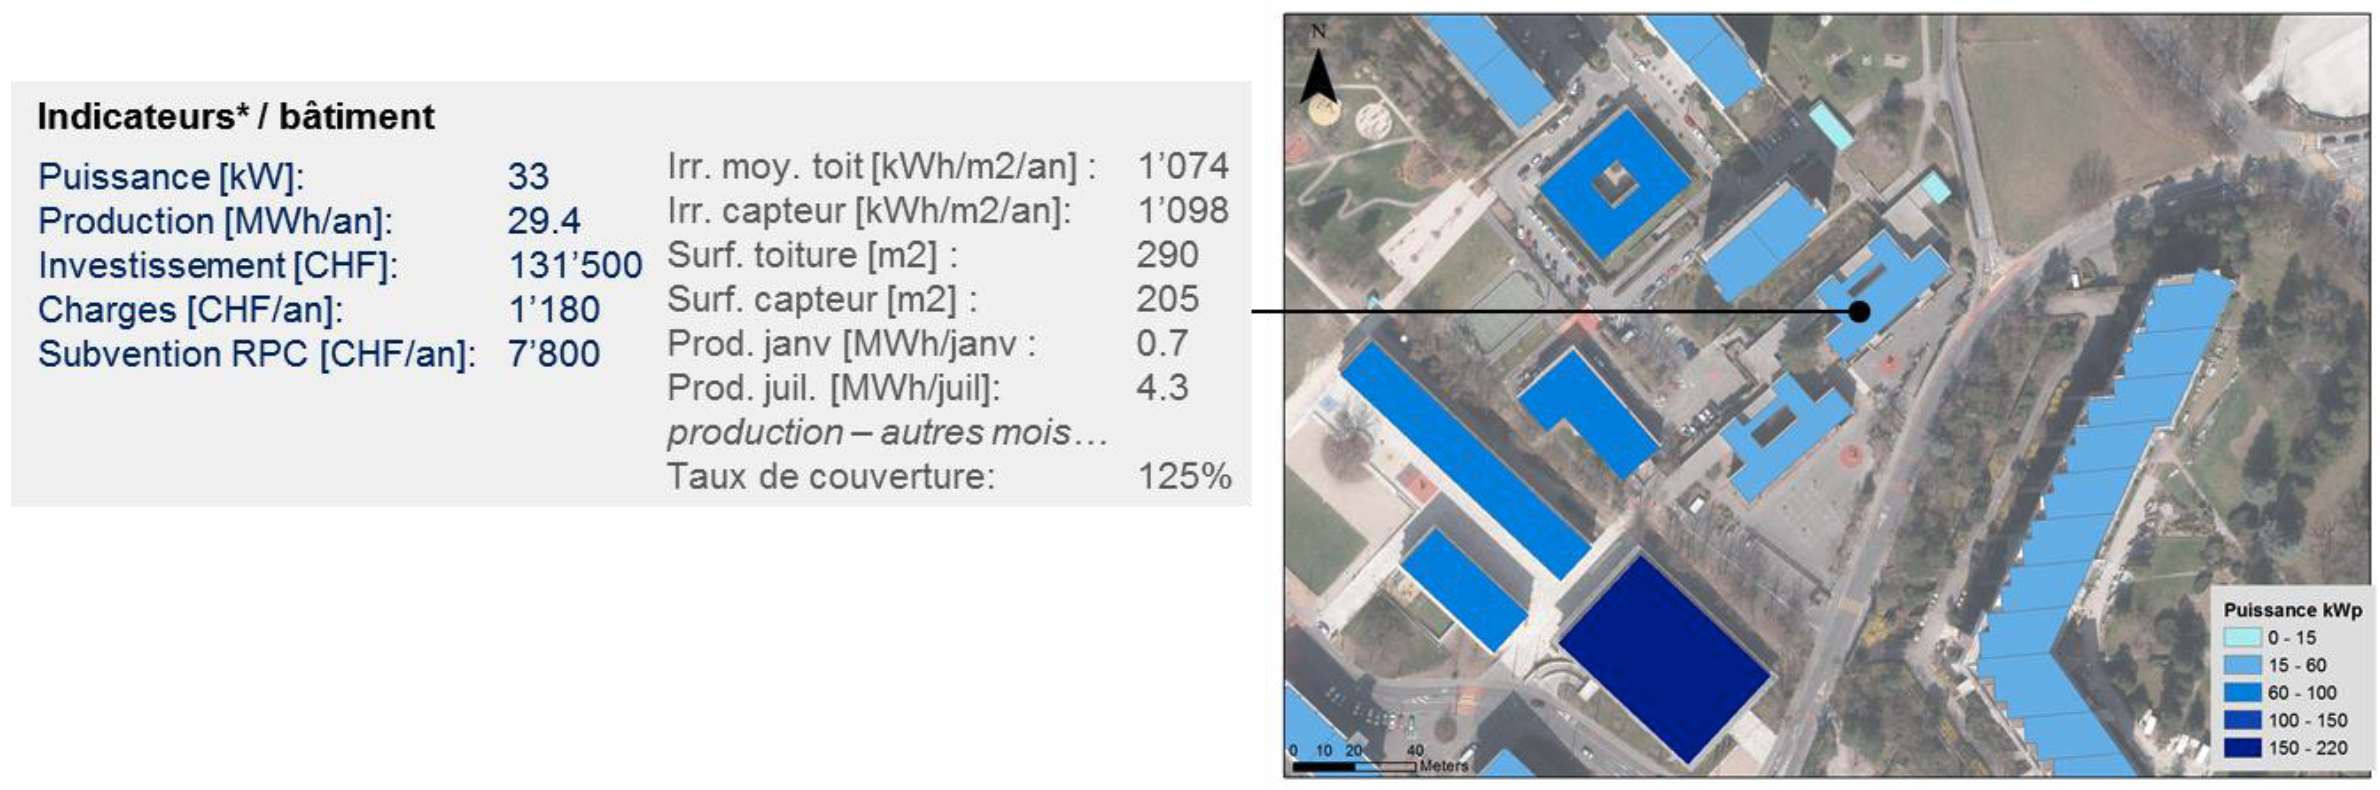
\includegraphics[width=1\linewidth]{02-main//figures/ch2/cadastre_solaire_2014.png}
    \caption{Image d'exemple avec une partie des informations disponibles par bâtiment \cite{desthieux_etude_2014}.}
    \label{fig:cadastre_solaire_2014}
\end{figure}

\par{En 2016, le cadastre a été mis à jour \cite{desthieux_solar_2018}. Les principales nouveautés sont :
\begin{itemize}
    \item L'utilisation des données \gls{lidar} de 2013 \cite{sitg_nuages_2013}
    \item L'amélioration des algorithmes de calcul du potentiel solaire
    \item Utilisation d'un cluster (24 machines) pour réaliser les calculs (environ 900h)
\end{itemize}}

\par{Dès 2018, plusieurs mises à jour \cite{desthieux_solar_2018} sont effectuées. Les principales nouveautés sont :
\begin{itemize}
    \item Prise en compte des toitures et des façades des bâtiments pour l'évaluation du potentiel solaire
    \item Amélioration des algorithmes de calcul du modèle de ciel
    \item Réécriture du code Matlab en Java
    \item Utilisation du cloud CTI IceBOUND
    \item Expansion du cadastre solaire au Grand Genève (canton de Genève, district de Nyon, et pôle métropolitain du Genevois Français)
\end{itemize}}

\par{En 2020, l'article \cite{stendardo_gpu-enabled_2020} de \citeauthor{stendardo_gpu-enabled_2020} aborde la question de l'optimisation des calculs pour le cadastre du Grand Genève. Les auteurs proposent l'utilisation des \acrshort{gpu} pour réduire considérablement les temps de traitement. Cette amélioration répond à un défi croissant : chaque nouvelle version du cadastre intègre davantage de données et requiert des calculs plus précis, ce qui allonge inévitablement les temps d'exécution. L'optimisation du code devient donc un aspect fondamental pour la viabilité du projet.}
\begin{figure}[H]
    \centering
    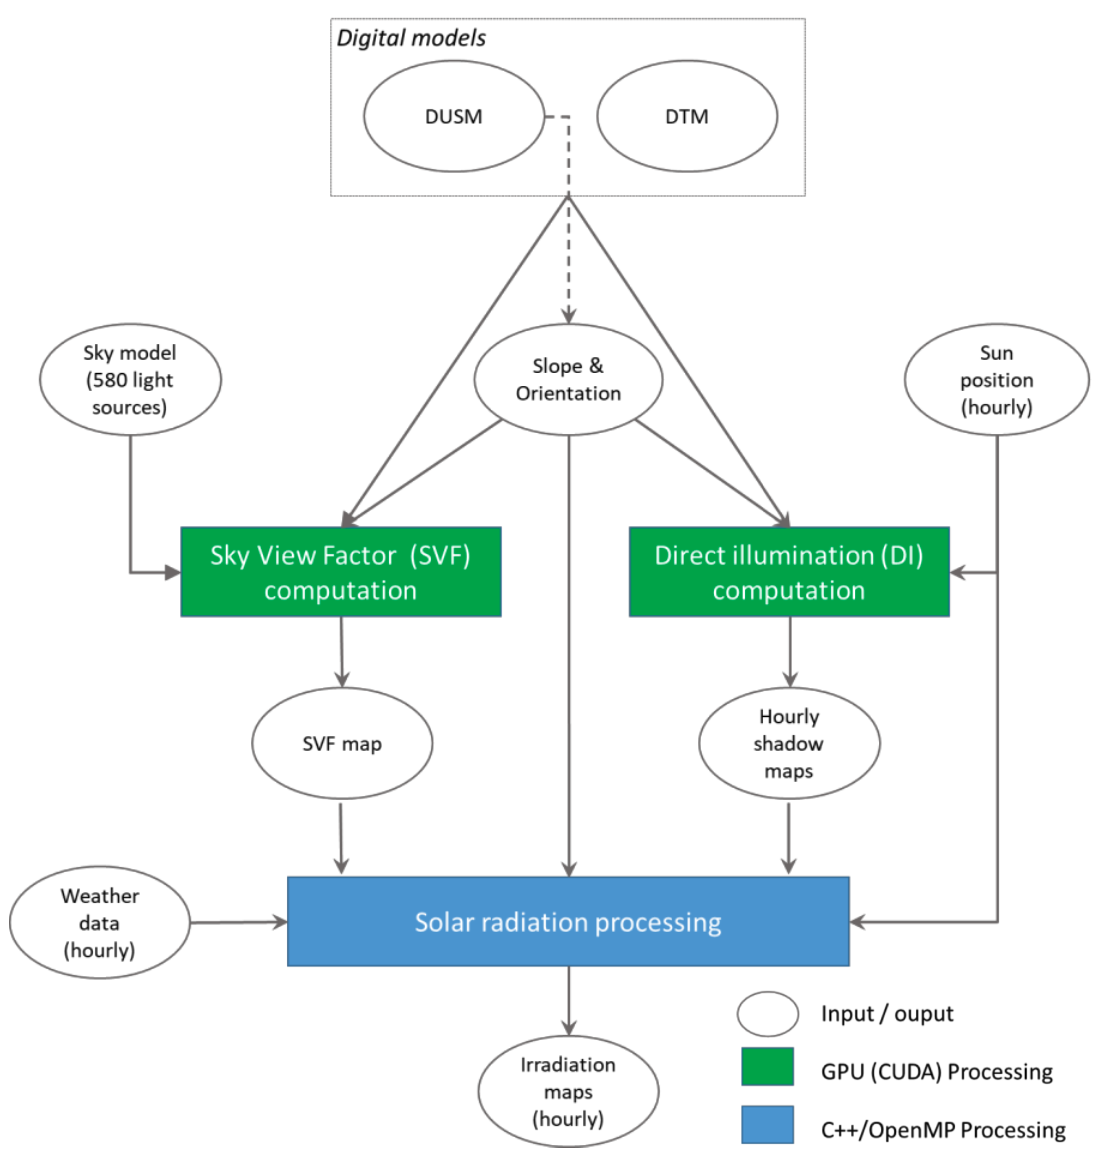
\includegraphics[width=1\linewidth]{02-main//figures/ch2/cadastre_solaire_gpu.png}
    \caption{Schéma pour le calcul d'une tuile \cite{stendardo_gpu-enabled_2020}}
    \label{fig:cadastre_solaire_gpu}
\end{figure}
\par{La Figure \ref{fig:cadastre_solaire_gpu} montre comment le traitement a été repensé pour chaque tuile de 3 x 3 km. Les parties du code Java qui pouvaient être massivement parallélisées ont été réécrites en CUDA \cite{nvidia_cuda_nodate}, ce qui permet de tirer parti des \acrshort{gpu} au lieu de s'appuyer uniquement sur les \acrshort{cpu}. Les autres parties critiques du code ont été optimisées en C++ \cite{noauthor_c_2025}. On peut voir sur la Figure \ref{fig:cadastre_solaire_gpu_evolution_temps} que cette approche a permis de réduire considérablement le temps de traitement par tuile.}

\begin{figure}[H]
    \centering
    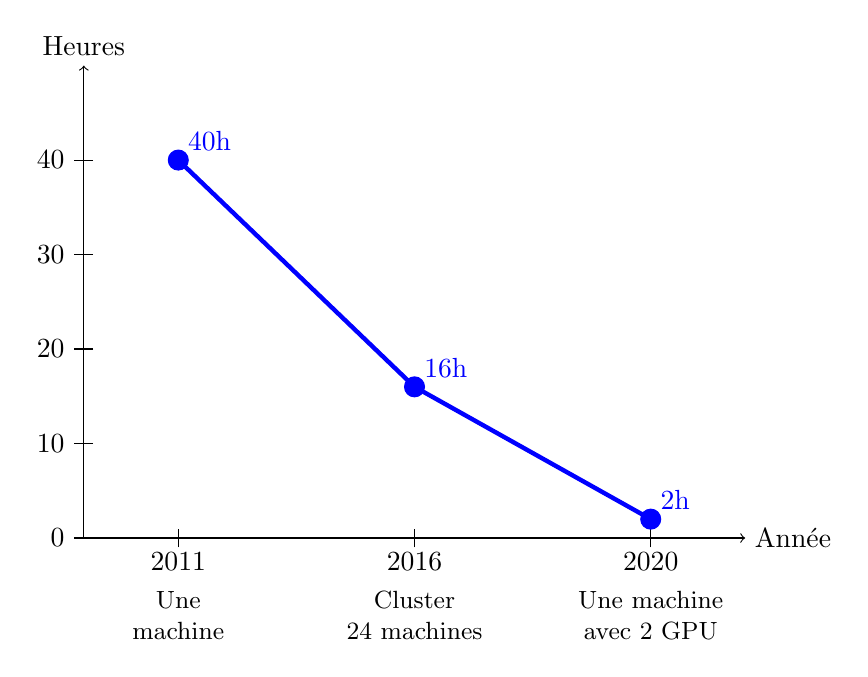
\begin{tikzpicture}[scale=1.2]
        % Axes
        \draw[->] (0,0) -- (7,0) node[right] {Année};
        \draw[->] (0,0) -- (0,5) node[above] {Heures};
        
        % Graduations - en commençant par 1 au lieu de 0
        \foreach \y in {1,2,3,4}
            \draw (0.1,\y) -- (-0.1,\y) node[left] {\y0};
        
        % Ajouter le 0 séparément
        \draw (0.1,0) -- (-0.1,0) node[left] {0};
        
        % Années
        \foreach \x/\year in {1/2011, 3.5/2016, 6/2020}
            \draw (\x,-0.1) -- (\x,0.1) node[below=5pt] {\year};
        
        % Données
        \draw[blue, ultra thick] (1,4) -- (3.5,1.6) -- (6,0.2);
        
        % Points
        \filldraw[blue] (1,4) circle (3pt) node[above right] {40h};
        \filldraw[blue] (3.5,1.6) circle (3pt) node[above right] {16h};
        \filldraw[blue] (6,0.2) circle (3pt) node[above right] {2h};
        
        % Annotations
        \node[align=center, font=\small, below] at (1,0) {\\\\Une\\machine};
        \node[align=center, font=\small, below] at (3.5,0) {\\\\Cluster\\24 machines};
        \node[align=center, font=\small, below] at (6,0) {\\\\Une machine\\avec 2 GPU};
    \end{tikzpicture}
    \caption{Évolution des temps de calcul par tuile pour le cadastre solaire (2011-2020).}
    \label{fig:cadastre_solaire_gpu_evolution_temps}
\end{figure}

\subsubsection{Données}
\par{Le cadastre genevois et du \gls{grandgeneve} \cite{desthieux_cadastre_nodate} utilisent plusieurs sources de données. Pour la région de Genève, \acrshort{sitg} a mis à disposition les données \gls{lidar} relevées les années:}
\begin{itemize}
    \item 2009 \cite{sitg_nuages_2009} avec une densité de 5 points au mètre carré. La précision altimétrique est de +/- 20 cm sur surface dure et la précision planimétrique est estimée à 30 cm environ.
    \item 2013 \cite{sitg_nuages_2013} avec une densité de 15 points au mètre carré. La précision altimétrique est de +/- 10 cm sur surface dure et la précision planimétrique est estimée à 20 cm environ.
    \item 2017 \cite{sitg_nuages_2017} avec une densité de 25 points au mètre carré. La précision altimétrique est de +/- 10 cm sur surface dure et la précision planimétrique est estimée à 20 cm environ.
\end{itemize}
\par{En ce qui concerne la région de Nyon, les données \gls{lidar} relevées en 2019 \cite{etat_de_vaud_lidar_nodate} et finalement, pour la France, les données \gls{lidar} relevées en 2014 \cite{ign_ign_nodate} par le \acrshort{ign}.}
\par{Les données vectorielles proviennent des mêmes fournisseurs de données et ne sont pas spécifiées dans les articles. Les données météo proviennent de Météonorm.}


\subsubsection{Méthodologie}

\par{La méthodologie \cite{desthieux_solar_2018} pour la création du cadastre suit les étapes suivantes :}
\begin{itemize}
    \item Collecte des données
    \item Construction du modèle 3D
    \item Calcul des ombrages
    \item Calcul de l'irradiation solaire en chaque point des toits et façades
    \item Calcul des indicateurs et visualisation des résultats
\end{itemize}

\par{La Figure \ref{fig:cadastre_solaire_methodologie} résume ces points.}
\begin{figure}[H]
    \centering
    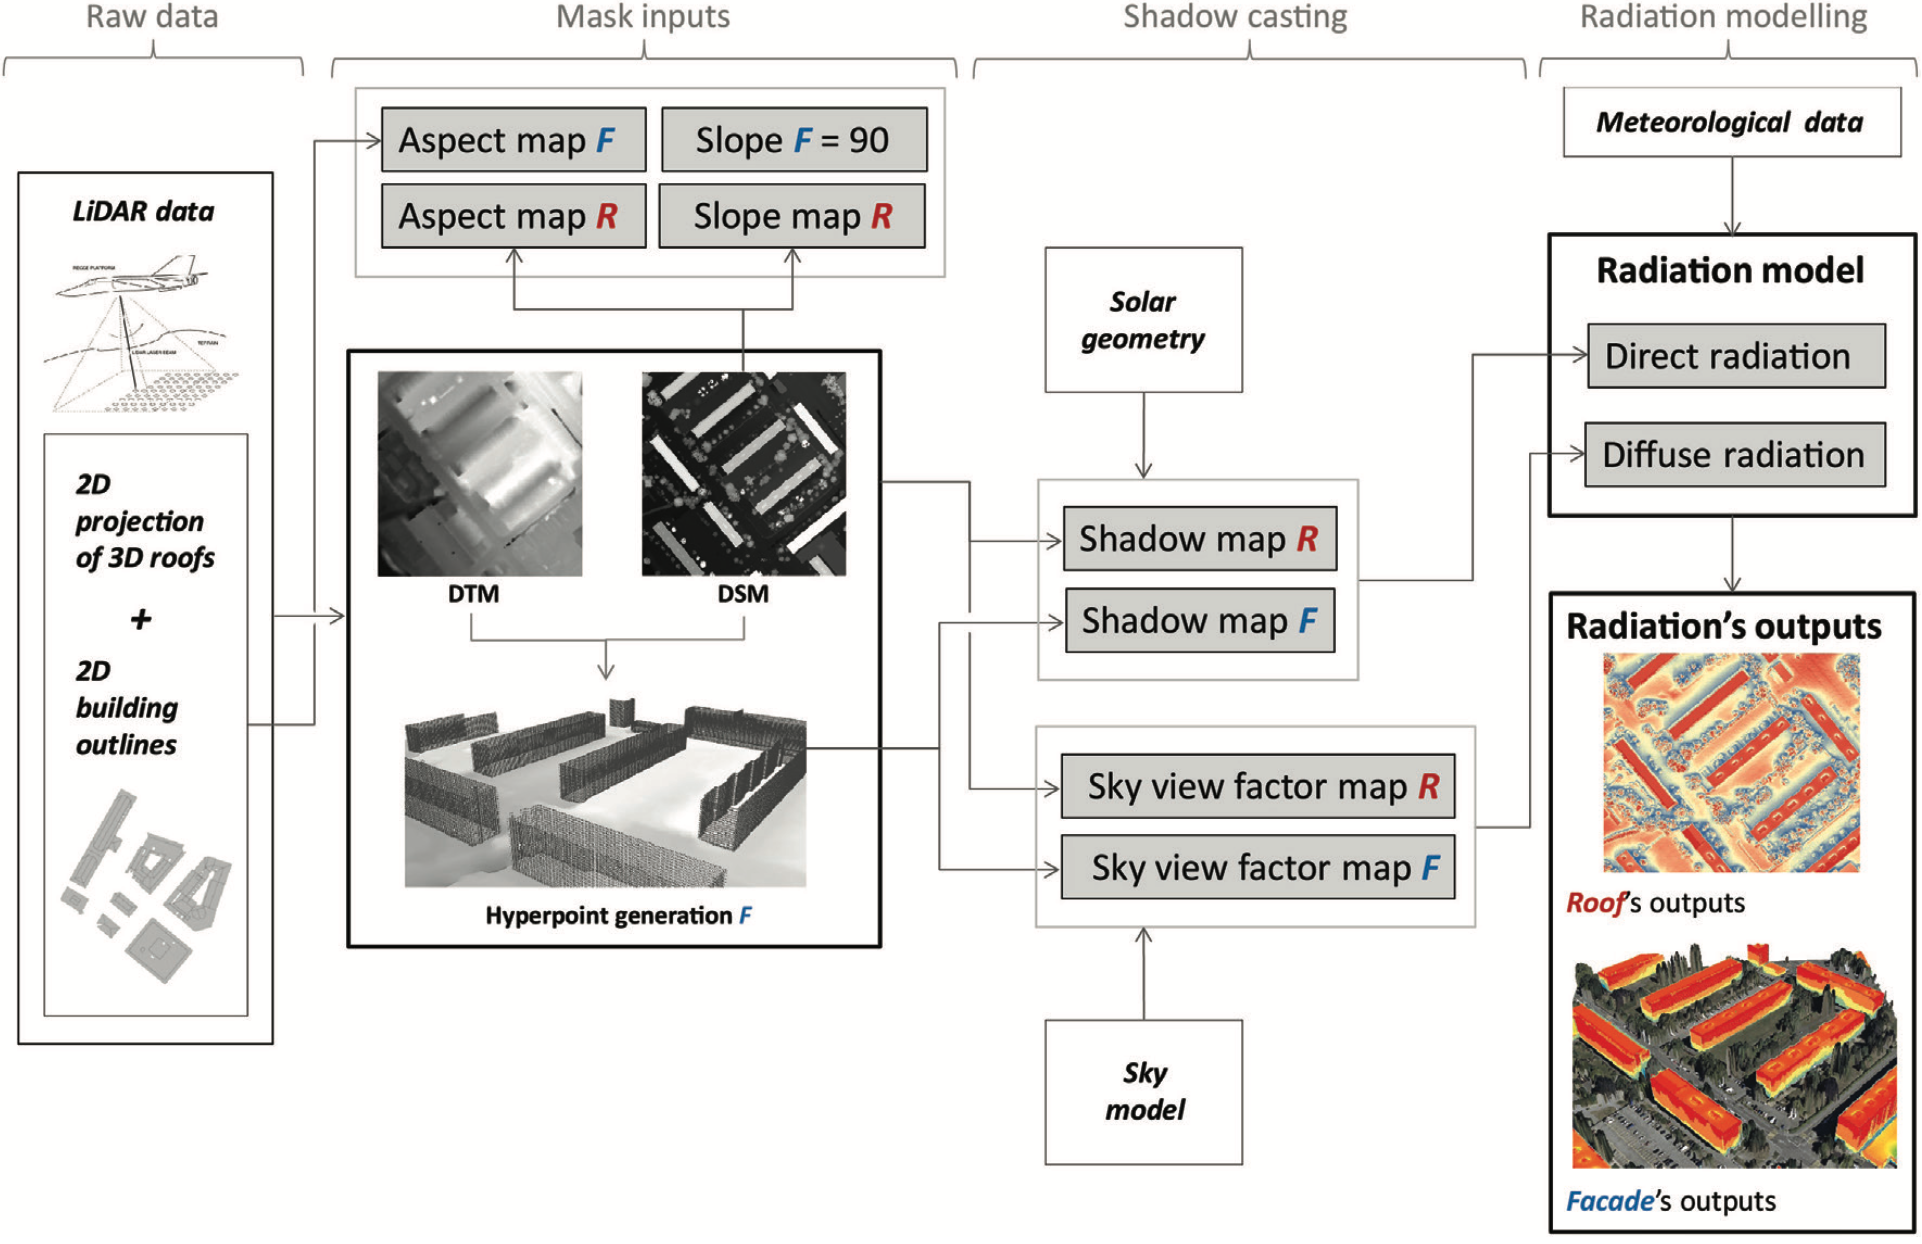
\includegraphics[width=1\linewidth]{02-main//figures/ch2/cadastre_solaire_methodologie.png}
    \caption{Méthodologie utilisée pour la création du cadastre solaire \cite{desthieux_solar_2018}}
    \label{fig:cadastre_solaire_methodologie}
\end{figure}

\paragraph{Collecte des données}
\par{La première étape est d'obtenir les données nécessaires ("Raw data" sur la Figure \ref{fig:cadastre_solaire_methodologie}). À partir des données \gls{lidar}, on construit deux modèles 3D de la ville : un modèle numérique de surface (\acrshort{mns} ou en anglais \acrshort{dsm}) qui représente la surface supérieure des bâtiments et de la végétation, et un modèle numérique de terrain (\acrshort{mnt} ou en anglais \acrshort{dtm}) qui représente le sol nu sans les bâtiments.}
\par{Les contours et empreintes des toits et bâtiments  sont aussi récupérés à partir de données cadastrales existantes, en 2D et 3D. Ils serviront à délimiter précisément les toits et façades.}

\paragraph{Construction du modèle 3D détaillé}
\par{La deuxième étape consiste à construire un modèle 3D détaillé de la ville ("mask inputs" sur la Figure \ref{fig:cadastre_solaire_methodologie}), qui servira de base aux calculs d'ensoleillement. Ce modèle est créé à partir des données récoltées à l'étape précédente.}
\par{Tout d'abord, le modèle numérique de surface (DSM) et le modèle numérique de terrain (DTM) sont transformés en images 3D appelées "rasters". Imaginez une grande grille recouvrant toute la ville, où chaque case de la grille (appelée "pixel") contient une valeur de hauteur. C'est exactement ce que sont le \acrshort{dsm} et le \acrshort{dtm} : des grandes grilles 3D où la hauteur de chaque point de la ville est enregistrée.}
\par{Ensuite, deux modèles 3D distincts sont créés : un pour les toits et un pour les façades. Pour cela, on combine le \acrshort{dsm} obtenu à partir des données \gls{lidar} avec les données cadastrales qui contiennent les contours des bâtiments. Cela permet d'avoir un modèle 3D, où chaque toit et chaque façade est représenté.}
\par{Pour chaque pixel du modèle 3D des toits, deux informations supplémentaires sont calculées : la pente (c'est-à-dire l'inclinaison) et l'orientation (nord, sud, est, ouest...). Ces deux paramètres sont très importants car ils influencent grandement la quantité d'énergie solaire reçue. Par exemple, un toit plat horizontal recevra plus de soleil qu'un toit très pentu orienté vers le nord.}
\par{Le modèle 3D des façades est un peu plus complexe à créer. En effet, un modèle "raster" comme celui des toits ne permet pas de bien représenter les surfaces verticales. Pour contourner ce problème, des points supplémentaires appelés "hyperpoints" sont ajoutés le long des façades (voir Figure \ref{fig:cadastre_solaire_hyperpoints}). Ils permettent de représenter chaque façade comme une série de points verticaux, sur lesquels on pourra ensuite calculer l'ensoleillement de manière précise.}
\begin{figure}[H]
    \centering
    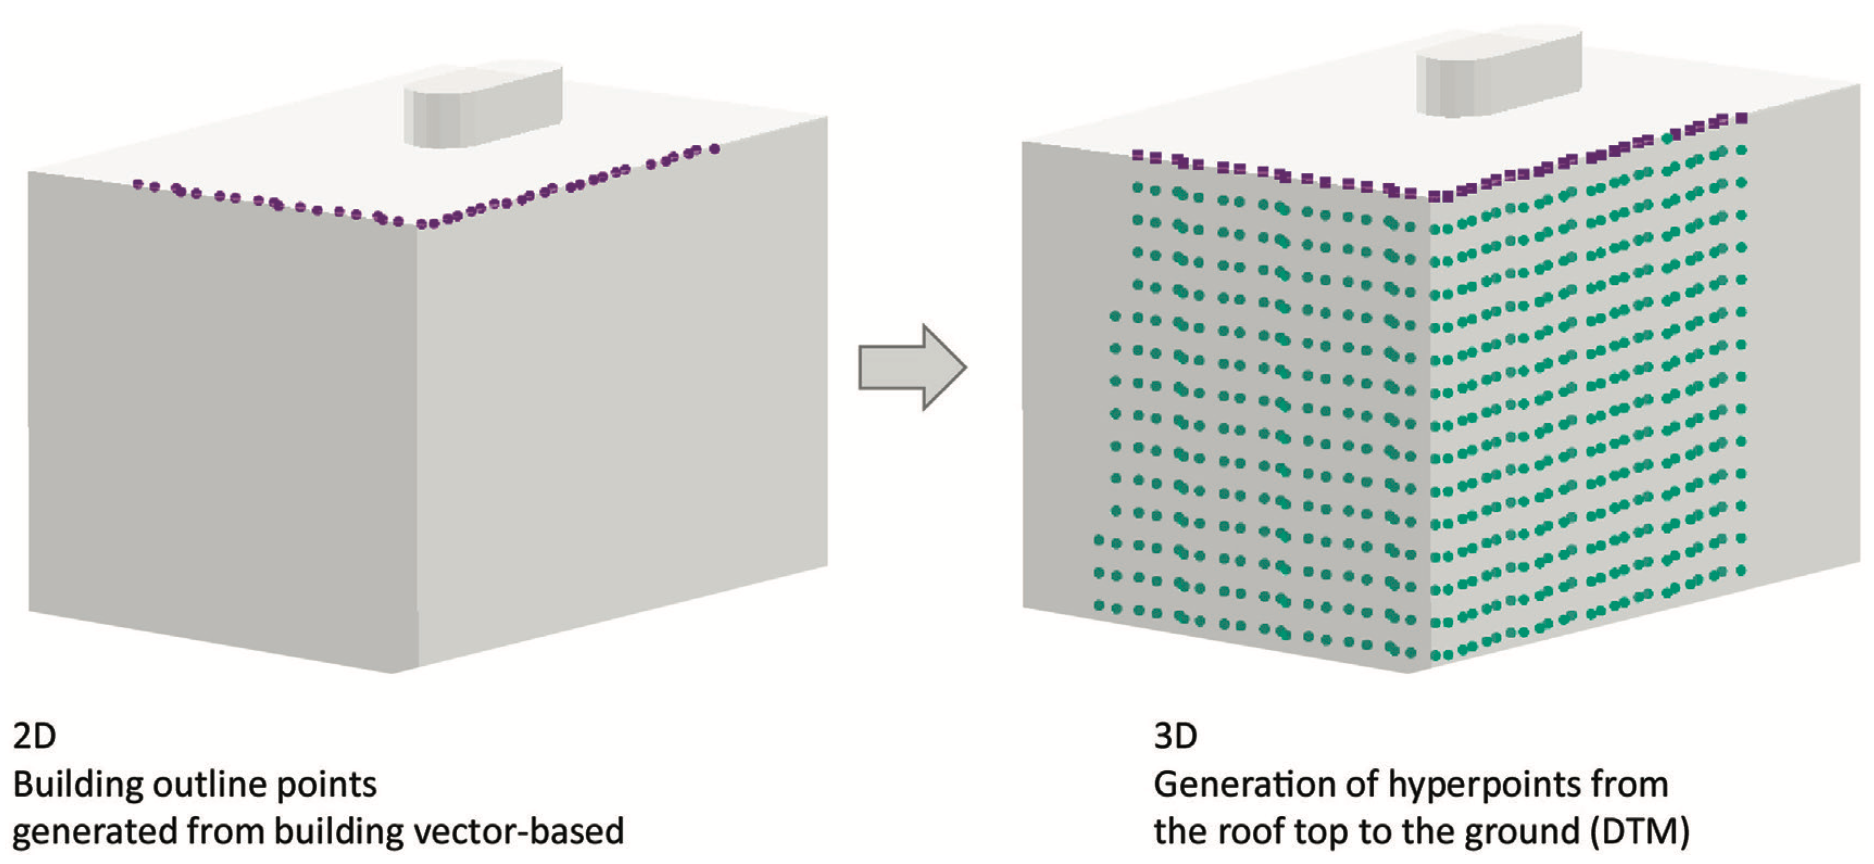
\includegraphics[width=1\linewidth]{02-main//figures/ch2/cadastre_solaire_hyperpoints.png}
    \caption{Méthode de création des hyperpoints sur les façades \cite{desthieux_solar_2018}}
    \label{fig:cadastre_solaire_hyperpoints}
\end{figure}
\par{Finalement, on obtient un jumeau numérique très détaillé de la ville, avec un modèle 3D distinct pour les toits et les façades. Ce jumeau numérique contient toutes les informations nécessaires (hauteur, pente, orientation) pour calculer finement l'ensoleillement en tout point. Les étapes suivantes vont s'appuyer sur ce modèle pour simuler les ombres portées et calculer le potentiel solaire.}

\paragraph{Calcul des zones d'ombre}
\par{La troisième étape consiste à calculer les zones d'ombre sur les toits et les façades des bâtiments (``mask inputs'' sur Figure \ref{fig:cadastre_solaire_methodologie}). Cette étape est cruciale car les zones ombragées ont un potentiel solaire significativement inférieur aux zones bien exposées au soleil.}
\par{Pour réaliser ce calcul, le jumeau numérique 3D de la ville créé précédemment est utilisé comme base. Ce modèle contient toutes les informations nécessaires sur la forme et la hauteur des bâtiments et du relief environnant. Un algorithme de simulation reproduit la course du soleil heure par heure tout au long de l'année, projetant les ombres correspondantes sur le modèle 3D.}
\par{L'ombrage représente l'un des facteurs les plus déterminants pour la performance d'une installation solaire. Pour analyser précisément son impact, trois catégories principales d'ombrages sont identifiées:}
\begin{itemize}
    \item Les ombrages proches: Causés par des éléments situés directement sur le toit comme les cheminées, antennes ou systèmes de ventilation.
    \item Les ombrages lointains: Proviennent du relief naturel (collines, montagnes) ou des grands bâtiments environnants. L'évaluation de leur impact nécessite une étude complète du masque solaire sur l'ensemble de l'année, car leur influence varie considérablement selon les saisons et la position du soleil.
    \item Les ombrages saisonniers: Générés par des éléments variables comme la végétation ou l'accumulation de neige. Ces ombrages évoluent au cours des saisons et nécessitent une gestion adaptative par un entretien régulier et une conception appropriée de l'installation.
\end{itemize}
\begin{figure}[H]
    \centering
    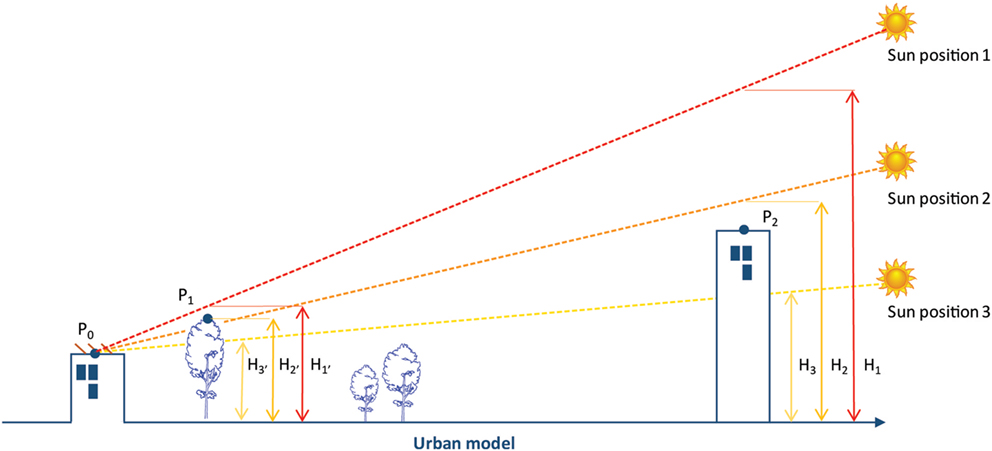
\includegraphics[width=1.00\linewidth]{02-main/figures/ch2/cadastre_solaire_ombrage.jpg}
    \caption{Illustration des différents types d'ombrages \cite{desthieux_solar_2018}}
    \label{fig:cadastre_solaire_ombrage}
\end{figure}
\par{La Figure \ref{fig:cadastre_solaire_ombrage} illustre ces concepts d'ombrage. À la position 1, le soleil n'est obstrué par aucun obstacle, donc le point $P_0$ reçoit un ensoleillement direct. À la position 2, un arbre projette une ombre sur $P_0$, créant un ombrage saisonnier dont l'intensité varie selon le type de végétation et la période de l'année. La position 3 représente une situation typique en milieu urbain où un bâtiment plus élevé projette une ombre sur les structures plus basses. Cette situation peut correspondre à un ombrage proche ou lointain selon la distance et les dimensions du bâtiment obstructif.}
\par{Le résultat de cette analyse produit des "cartes d'ombrage" indiquant, pour chaque heure de la journée, quelles zones des toits et façades sont à l'ombre ou exposées au soleil. Ces cartes constituent une donnée fondamentale pour le calcul final du potentiel solaire.}
\par{En complément de l'ombrage direct, le modèle calcule également le "facteur de vue du ciel" (sky view factor). Ce paramètre mesure la portion de ciel visible depuis un point précis de la ville. Conceptuellement, si une personne se tient à un point donné (représenté en rouge sur la Figure \ref{fig:cadastre_solaire_svf}) et observe le ciel dans toutes les directions, certaines portions seront masquées par les bâtiments, la végétation, ou le relief.}
\begin{figure}[H]
    \centering
    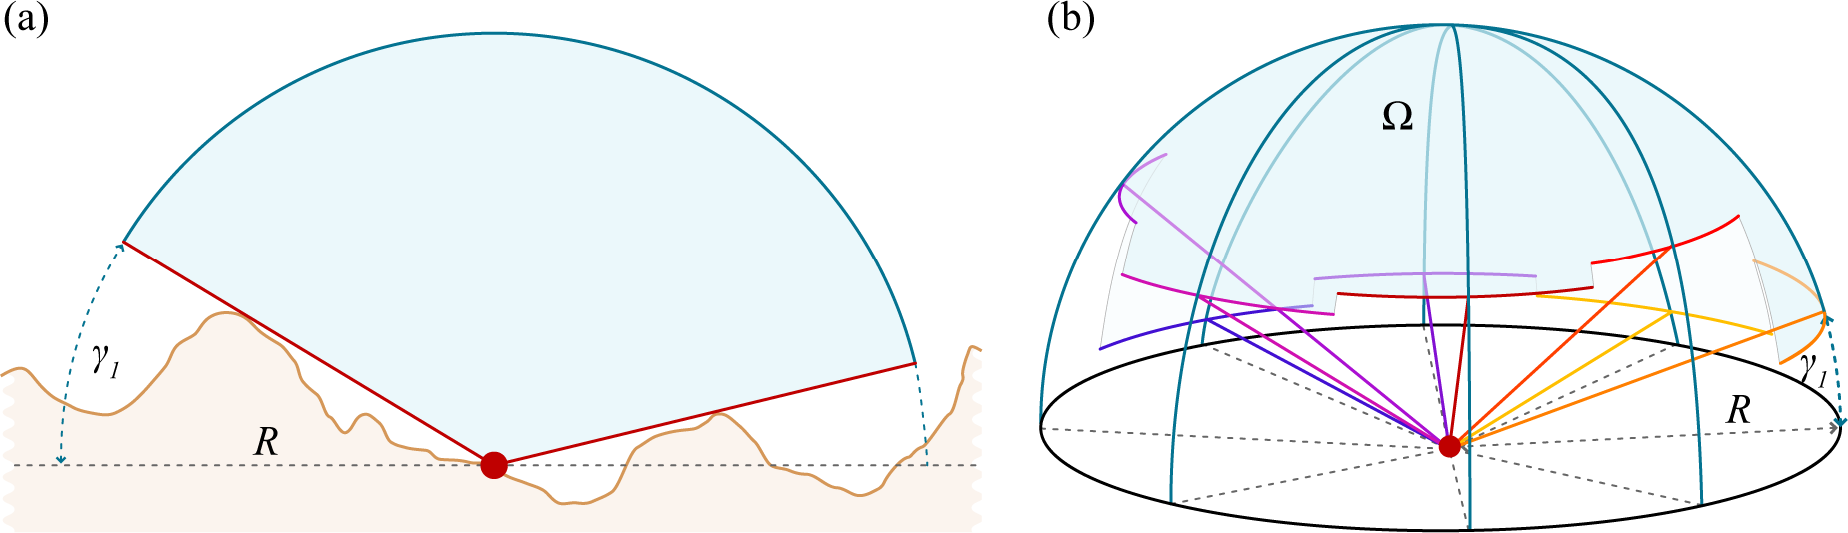
\includegraphics[width=1\linewidth]{02-main/figures/ch2/ch2_cadastre_solaire_svf.png}
    \caption{Le sky view factor (SVF) indique la proportion de ciel visible depuis un point \cite{zaksek_sky-view_2011}}
    \label{fig:cadastre_solaire_svf}
\end{figure}
\par{Le facteur de vue du ciel est exprimé en pourcentage: 100\% correspond à une vue entièrement dégagée (comme au sommet d'une tour ou d'une colline), tandis que 0\% indique un point complètement obstrué (sous un porche ou dans un tunnel). Ce facteur est crucial car il détermine la quantité de lumière naturelle et de rayonnement solaire diffus (indirect) reçue en ce point, en complément du rayonnement direct.}
\par{L'intégration des cartes d'ombrage avec le facteur de vue du ciel fournit une caractérisation complète des conditions d'ensoleillement pour chaque point de la ville. Cette analyse prend en compte à la fois les ombres portées par les obstacles proches et les masques créés par les éléments lointains, constituant ainsi une base solide pour le calcul définitif du potentiel solaire.}

\paragraph{Modélisation du rayonnement solaire}
\par{La quatrième étape consiste à modéliser la quantité d'énergie solaire reçue en chaque point des toits et des façades (``Radiation modelling'' sur Figure \ref{fig:cadastre_solaire_methodologie}), en tenant compte des conditions météorologiques locales et de la position du soleil dans le ciel.}
\par{Pour cela, on récupère tout d'abord des données météorologiques précises pour la zone étudiée :
\begin{itemize}
    \item Le rayonnement solaire global, c'est-à-dire la quantité totale d'énergie solaire reçue sur une surface horizontale.
    \item La part de rayonnement qui arrive en ligne droite du soleil (rayonnement direct).
    \item La part de rayonnement qui arrive de façon indirecte, après avoir été diffusée par les nuages et l'atmosphère (rayonnement diffus).
\end{itemize}}
\par{Ensuite, on utilise des modèles qui reproduisent la position exacte du soleil dans le ciel à chaque heure de la journée et à chaque période de l'année. Cela permet de calculer l'angle avec lequel les rayons du soleil frappent chaque point des toits et des façades.}
\par{En effet, la quantité d'énergie reçue en un point dépend fortement de son orientation (est, sud, ouest...) et de son inclinaison (surface horizontale, verticale ou inclinée). Un point orienté plein sud et incliné à 45° recevra par exemple beaucoup plus d'énergie qu'une façade verticale orientée au nord.}
\par{Les modèles de rayonnement utilisent des équations mathématiques pour calculer précisément la quantité d'énergie directe et diffuse reçue en chaque point, en fonction de tous ces paramètres.}
\par{De plus, ces modèles prennent aussi en compte les effets d'ombrage calculés à l'étape précédente. Ainsi, un point sera considéré comme ne recevant aucune énergie directe s'il est à l'ombre à l'instant considéré.}
\par{Ils intègrent également le "facteur de vue du ciel", qui traduit la portion de ciel visible depuis chaque point. Moins il y a de ciel visible (à cause des bâtiments et du relief alentour), moins il y aura de rayonnement diffus reçu.}
\par{Au final, on obtient une estimation très fine de la quantité d'énergie solaire reçue par chaque mètre carré des toits et façades, heure par heure, tout au long de l'année. Cela permet ensuite de sélectionner les zones les plus intéressantes pour installer des panneaux solaires par exemple.}

\paragraph{Résultats de la simulation}
\par{À la fin de tout ce processus, on obtient des résultats concrets et utilisables sous plusieurs formes. Ces résultats (``Roof outputs'' et ``façade outputs'' sur Figure \ref{fig:cadastre_solaire_methodologie}) sont :
\begin{itemize}
    \item Des cartes de rayonnement solaire pour les toits et façades
    \item Des valeurs d'énergie regroupées par pan de toit, façade, et bâtiment entier
    \item Des indicateurs pratiques comme la production d'énergie possible et la rentabilité économique
\end{itemize}}

\subsubsection{Résultats principaux}
\par{Tous les résultats sont disponibles pour les citoyens et les professionnels sur le géoportail cartographique de \acrshort{sitg} (Figure \ref{fig:cadastre_solaire_couche_vec_sitg}). Ils peuvent être affichés sous forme de couches cartographiques, au même titre que
d'autres données territoriales.}
\begin{figure}[H]
    \centering
    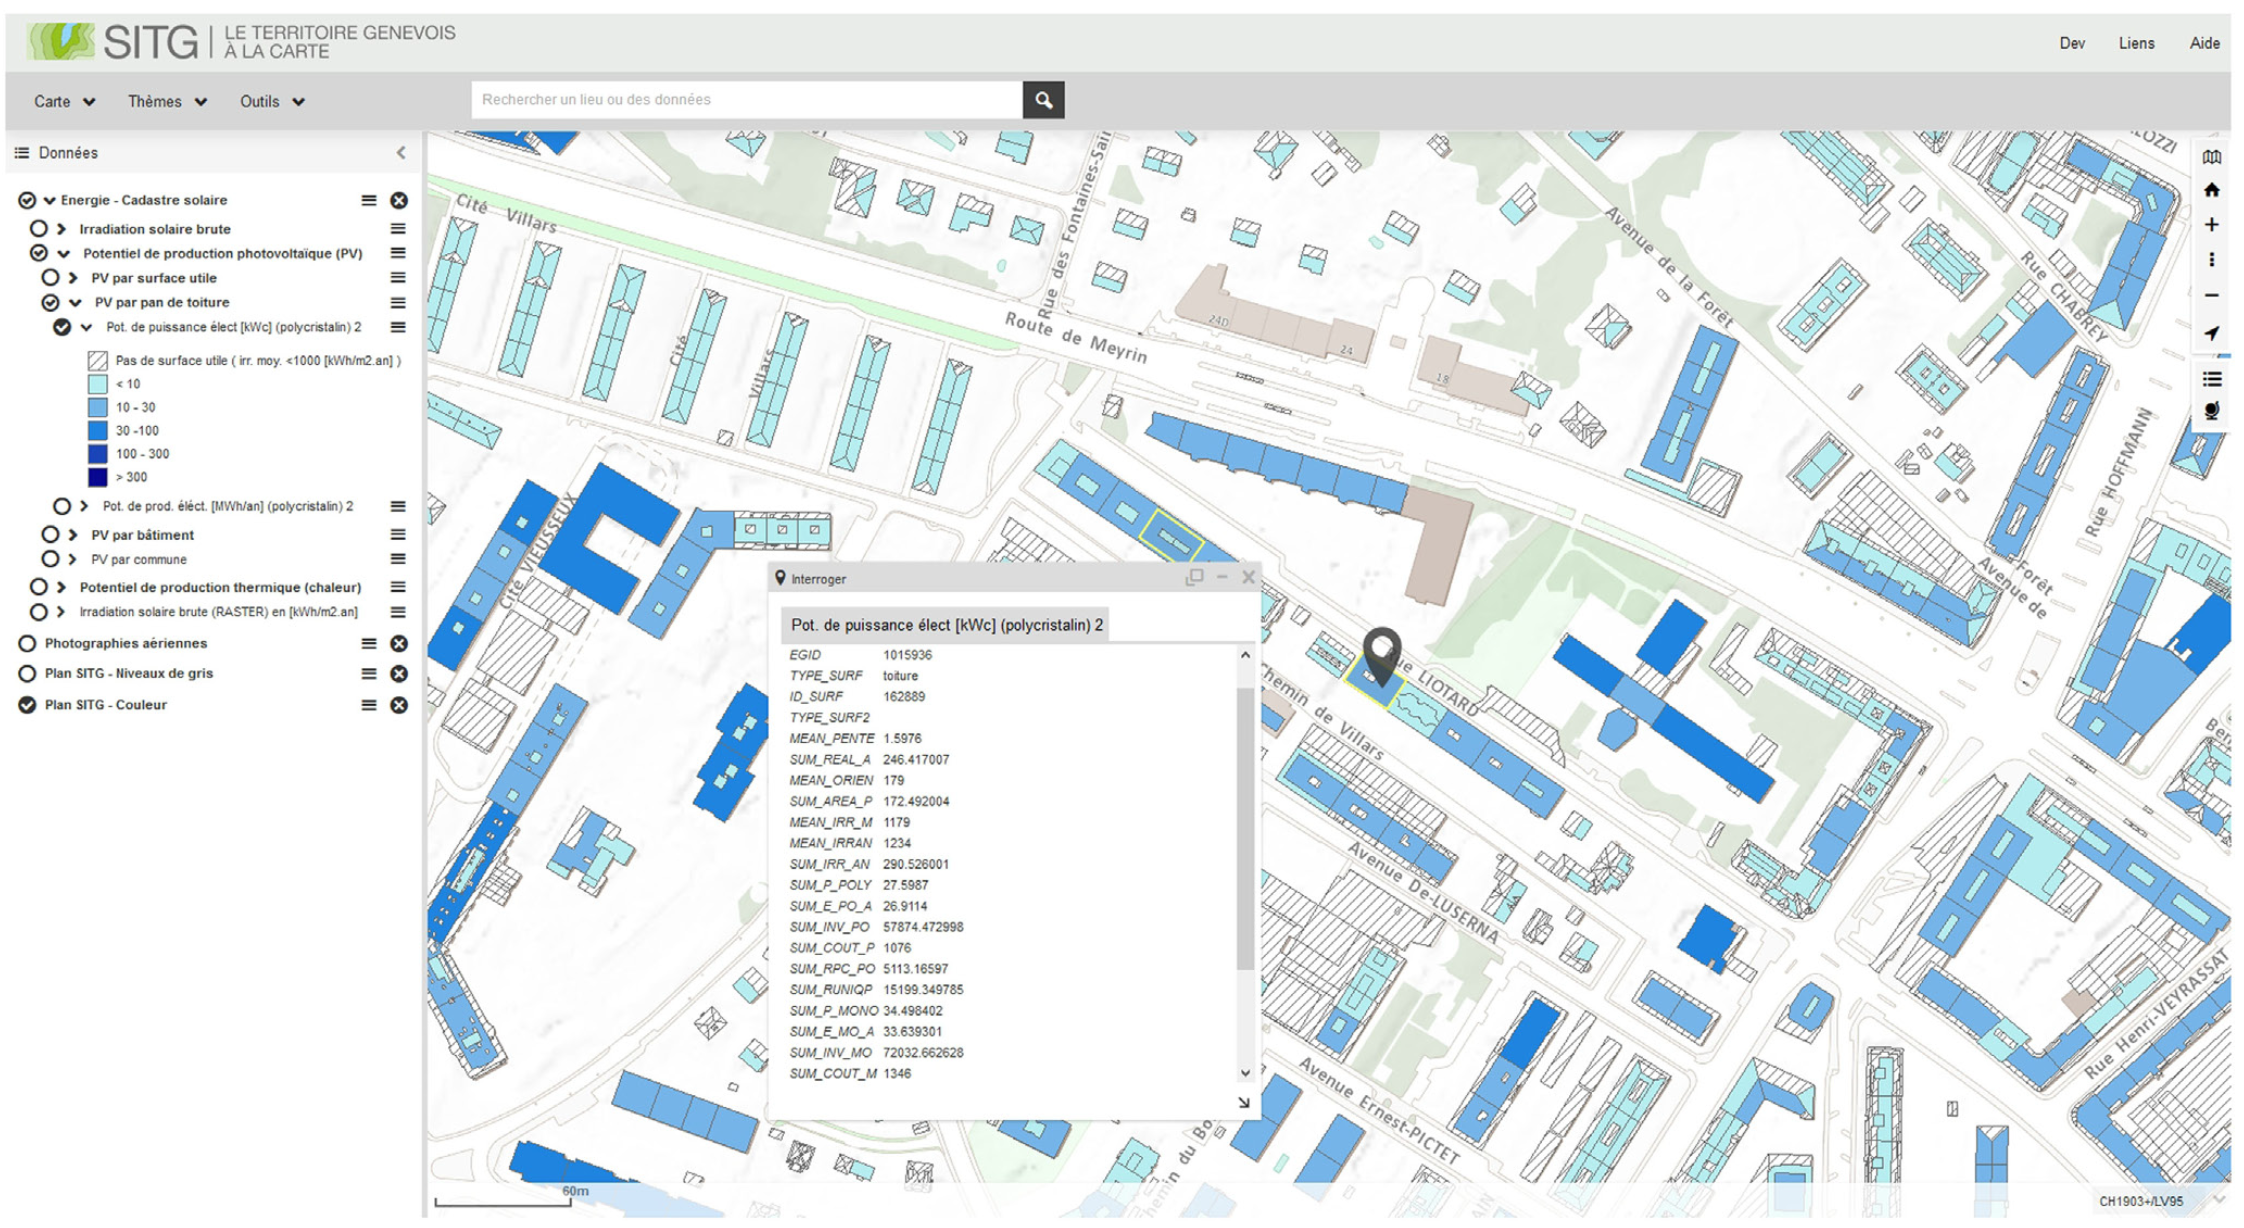
\includegraphics[width=1\linewidth]{02-main//figures/ch2/cadastre_solaire_couche_vec_sitg.png}
    \caption{Visualisation des couches vectorielles sur l'interface \acrshort{sitg} \cite{desthieux_solar_2018}}
    \label{fig:cadastre_solaire_couche_vec_sitg}
\end{figure}
\par{Un site web dédié au cadastre solaire a également été créé (Figure \ref{fig:cadastre_solaire_sitg_labs}). Il permet à chacun de rechercher une adresse et de visualiser très simplement le potentiel solaire du bâtiment correspondant, ainsi que des estimations de production d'énergie et de rentabilité économique.}
\begin{figure}[H]
    \centering
    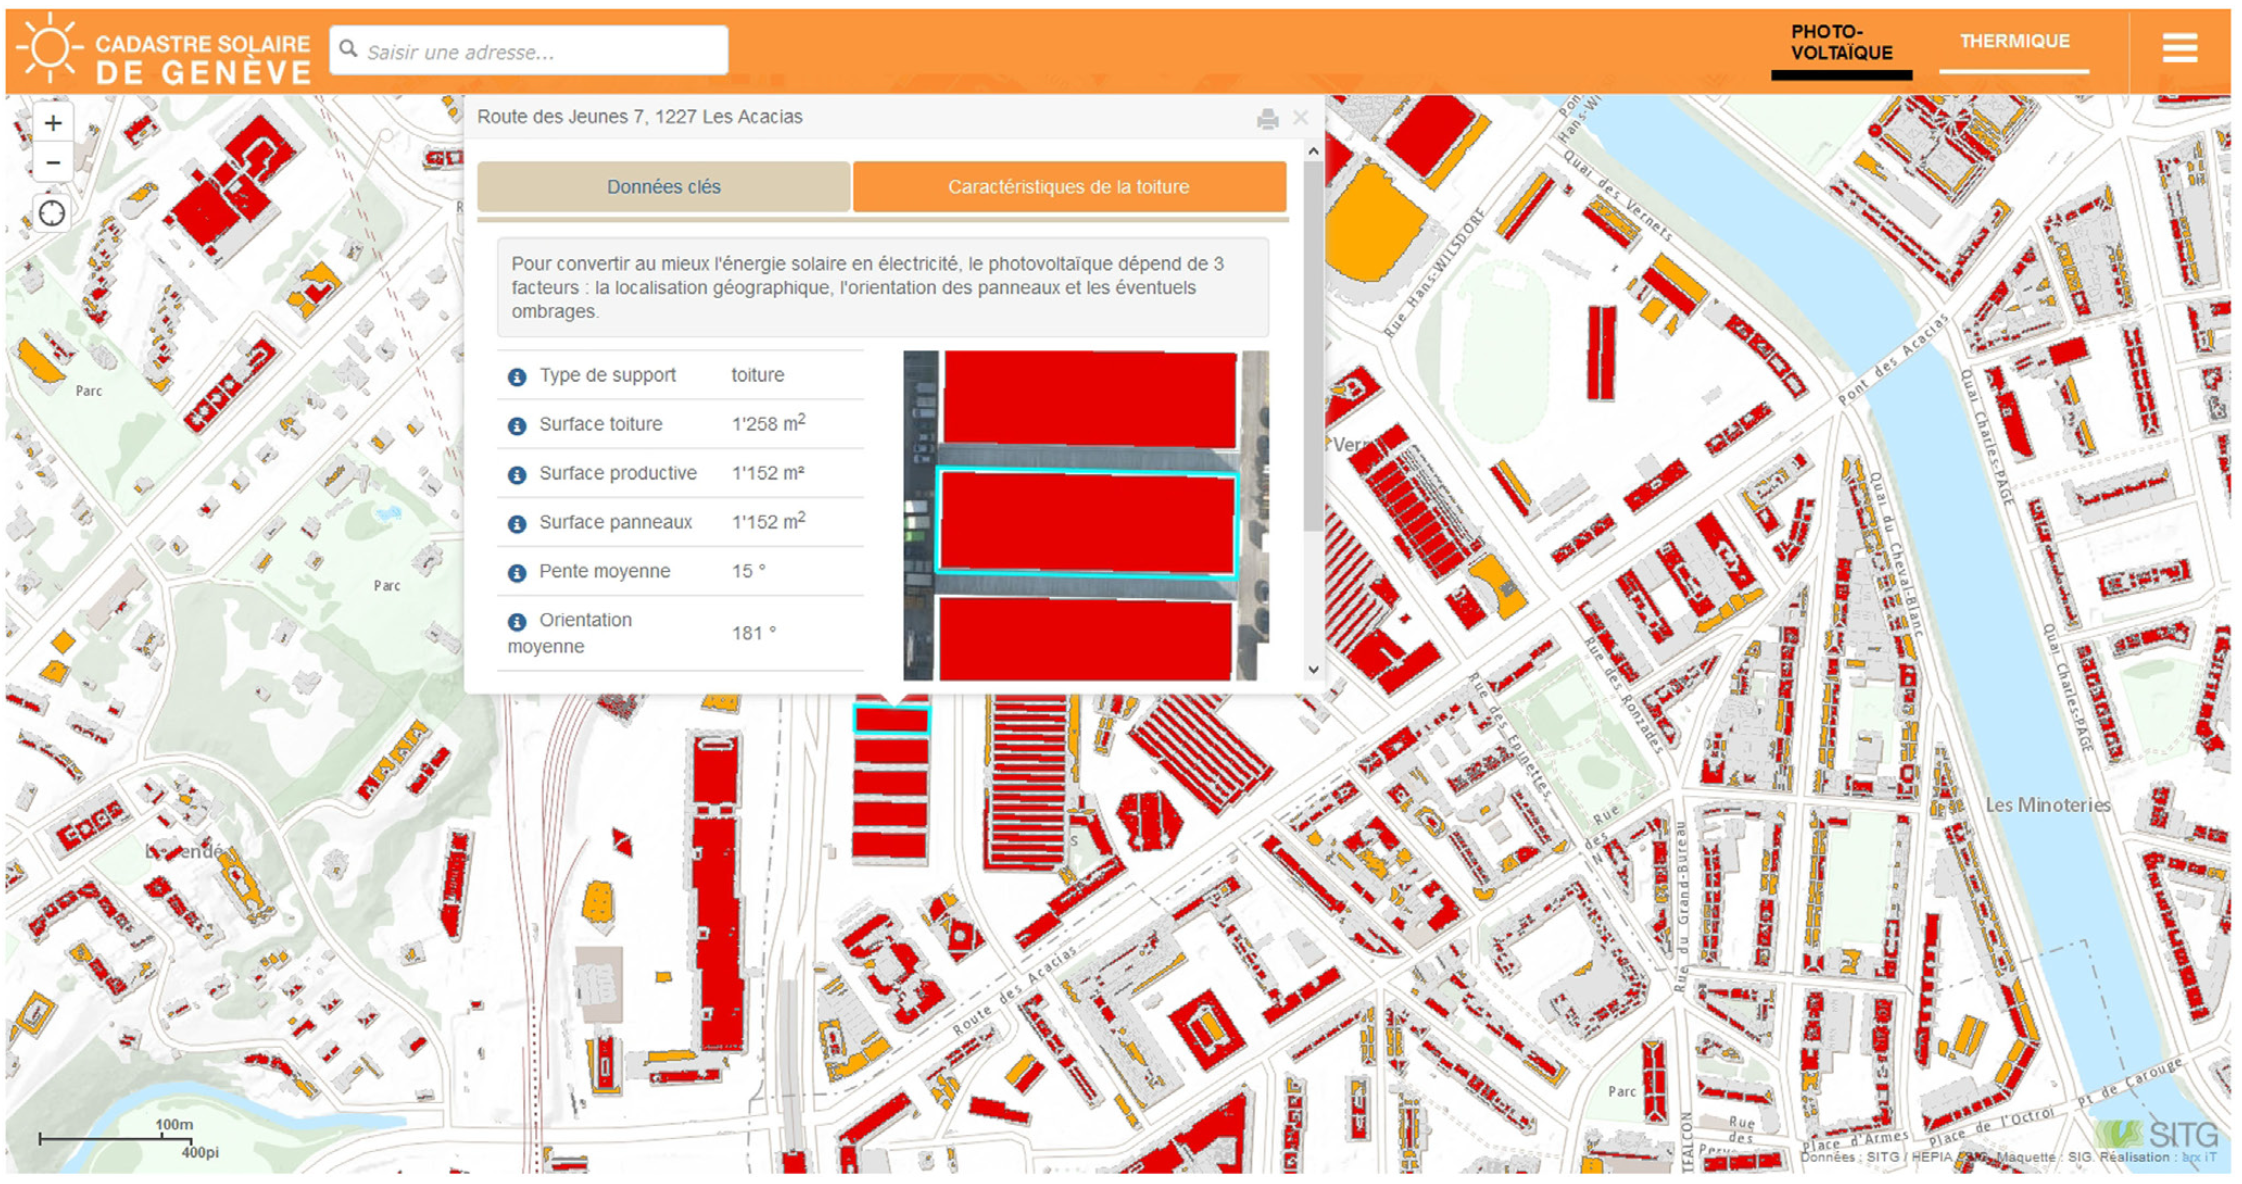
\includegraphics[width=1\linewidth]{02-main//figures/ch2/cadastre_solaire_sitg_labs.png}
    \caption{Interface utilisateur du cadastre solaire destinée au grand public \cite{desthieux_solar_2018}}
    \label{fig:cadastre_solaire_sitg_labs}
\end{figure}
\par{En rendant ces informations facilement accessibles à tous, le cadastre solaire devient un outil précieux pour encourager le développement de l'énergie solaire à Genève, que ce soit pour des projets individuels ou des planifications à grande échelle.}

\subsubsection{Discussion et limites}
\par{L'article de \citeauthor{desthieux_solar_2018} \cite{desthieux_solar_2018} présente une méthodologie complète pour évaluer le potentiel solaire d'une région. Cette approche explore notamment le potentiel des façades, qui constitue un gisement énergétique intéressant mais encore peu exploité. Dans le cadre de ce travail, les façades ne sont pas considérées, leur utilisation étant souvent limitée par des contraintes esthétiques, légales (notamment pour les bâtiments protégés) ou simplement par méconnaissance de leurs avantages. Si certains bâtiments récents intègrent désormais des panneaux solaires en façade, ces installations sont relativement rares.}
\par{Le calculateur a été validée de manière indépendante par l'Université de Genève, ce qui confirme la robustesse de la méthodologie. Un atout majeur réside dans l'utilisation des données relatives aux superstructures \cite{sitg_superstructures_nodate}, qui permet de prendre en compte les ombres projetées par ces éléments sur le reste de la toiture. Cependant, cette couche de données présente certaines limitations, la plupart des toitures comportent des éléments techniques tels que des gaines de ventilation ou des monoblocs qui ne sont pas systématiquement répertoriés dans la couche des superstructures. Ces surfaces pourraient potentiellement être considérées comme utilisables pour l'installation de panneaux solaires, puisqu'elles ne sont pas formellement classées comme superstructures. En définitive, c'est le niveau d'irradiation solaire et la présence ou non d'ombrage qui déterminent véritablement si une surface peut être exploitée efficacement pour la production d'énergie solaire.}

% -----------------------------------------------------------------------------
\subsection{ToitSolaire}

\par{Ce chapitre présente l'application toitsolaire.ch \cite{bfe_wie_nodate} et sa documentation technique \cite{klauser_energie_nodate} qui a été rédigée par l'Office fédéral de l'énergie (\acrshort{ofen}) ainsi que Meteotest \cite{meteotest_wir_2025}.}

\subsubsection{Contexte et objectifs}
\par{L'application toitsolaire.ch, développée par l'\acrshort{ofen}, constitue un cadastre solaire pour l'ensemble du territoire suisse et sert d'instrument d'encouragement pour l'utilisation de l'énergie solaire.}

\par{Ce projet s'inscrit dans la volonté fédérale de favoriser la transition énergétique en fournissant aux propriétaires et aux professionnels un outil permettant d'évaluer rapidement le potentiel solaire des toitures et des façades des bâtiments suisses. L'objectif principal est d'offrir une plateforme en ligne accessible qui présente de manière claire et précise le potentiel d'exploitation de l'énergie solaire pour chaque bâtiment, tant sur les toitures (toitsolaire.ch) que sur les façades (facade-au-soleil.ch).}

\subsubsection{Données}
\par{Le projet s'appuie sur trois types de données principales :}
\begin{itemize}
    \item Données climatiques
    \begin{itemize}
        \item Rayonnement solaire et températures (2011-2020) avec résolution d'environ 2 km, fournies par MétéoSuisse et dérivées de données satellitaires
    \end{itemize}
    \item Données géographiques
    \begin{itemize}
        \item Géométries des bâtiments en 3D (toits et façades) issues du modèle swissBUILDINGS3D 2.0
        \item Modèles numériques de terrain (swissALTI3D, resolution 2m)
        \item Modèles numériques de surface (swissSURFACE3D, résolution 0,5m)
        \item Modèle SRTM (résolution environ 100m)
    \end{itemize}
    \item Données statistiques
        \begin{itemize}
        \item Registre fédéral des bâtiments et des logements (RegBL) pour estimer les besoins en chaleur des bâtiments
        \end{itemize}
    \end{itemize}

\subsubsection{Méthodologie}
\par{Le traitement des données commence par l'analyse des géométries, suivi par le calcul du rayonnement solaire sur les surfaces et se termine par leur classification.}

\paragraph{Traitement des géométries}
\par{Les données 3D des bâtiments sont converties en polygones 2D pour les toits (vue d'oiseau) et polylignes 2D pour les façades. L'orientation, l'inclinaison et la surface de chaque pan de toit sont calculées.}

\paragraph{Calcul du rayonnement solaire}
Trois horizons d'ombrage sont calculés pour chaque surface :
\begin{itemize}
    \item Ombrage lointain (montagnes, collines) dans un rayon de 25 km
    \item Ombrage moyen (voisinage) dans un rayon de 1 km
    \item Ombrage proche (local) dans un rayon de 100 m
\end{itemize}
\par{Le rayonnement solaire sur les surfaces inclinées est calculé à l'aide du modèle anisotrope de Perez, qui tient compte du rayonnement direct, diffus et réfléchi. Les calculs sont effectués heure par heure sur la période 2011-2020.}

\paragraph{Calcul des rendements photovoltaïque et thermique}
\par{Le rendement électrique est calculé en multipliant le rayonnement solaire total par un rendement de module de 19\% et un ratio de performance de 80\%. Pour le solaire thermique, la méthode est plus complexe :}
\begin{itemize}
    \item Estimation des besoins en chaleur du bâtiment à partir des données du RegBL
    \item Dimensionnement d'une installation solaire thermique adaptée à ces besoins
    \item Calcul du rendement thermique à l'aide d'une formule d'approximation validée
    \item Conversion en métriques pratiques (nombre de douches possibles, pourcentage des besoins de chauffage couverts)
\end{itemize}

\paragraph{Classification}
\par{Les surfaces sont classées selon leur potentiel solaire, de "faible" à "excellent", en fonction du rayonnement solaire annuel moyen :}
\begin{itemize}
    \item Pour les toits : < 800, 800-1000, 1000-1200, 1200-1400, > 1400 kWh/m²/an
    \item Pour les façades : < 600, 600-800, 800-1000, 1000-1200, > 1200 kWh/m²/an
\end{itemize}

\subsubsection{Résultats principaux}
\par{Le projet a permis d'analyser environ 10 millions de pans de toit en Suisse, fournissant pour chacun des données géométriques et le potentiel solaire (\acrshort{pv} et solaire thermique) comme données principales.}
\paragraph{Données géométriques} Surface utilisable, orientation et inclinaison.
\paragraph{Potentiel photovoltaïque}
\begin{itemize}
    \item Rayonnement solaire global moyen (kWh/m²/an)
    \item Rayonnement solaire global total (kWh/an)
    \item Production électrique estimée (kWh/an)
\end{itemize}
\paragraph{Potentiel thermique solaire}
\begin{itemize}
    \item Rayonnement solaire global moyen et total
    \item Production thermique estimée
    \item Pourcentage des besoins de chauffage couverts
\end{itemize}
\paragraph{Classification}
\par{Catégorisation de chaque surface selon son aptitude à l'exploitation solaire.}
\paragraph{Paramètres mensuels}
\par{Pour chaque mois, des paramètres permettent de calculer le rayonnement sur surface inclinée à partir du rayonnement horizontal direct et diffus.}
\subsubsection{Discussion et limites}
\par{L'objectif de cet outil est très similaire au cadastre solaire genevois mais pour toute la Suisse. Il a les mêmes limites en ce qui concerne les superstructures des toitures, c'est-à-dire que les éléments de toiture qui ne sont pas renseignés dans la superstructure, seront considérés comme surface apte pour la mise en place de panneaux solaire.}
\par{La modélisation de la météo semble plus sophistiquée que celle du cadastre genevois. L'actualisation des données va dépendre principalement des relevés \gls{lidar} réalisés par swisstopo, mais en principe ceux-ci sont plus fréquents que pour le cadastre solaire genevois}

% -----------------------------------------------------------------------------
% -----------------------------------------------------------------------------
\section{Approche machine learning}

\par{Ce chapitre va permettre d'explorer l'état de l'art en vision par ordinateur appliqué aux données géomatiques.}

% -----------------------------------------------------------------------------
\subsection{Détection des objets présents sur les toitures et identification des espaces libres}
\label{subsec:stdl_analyse}
\vspace{2mm}
\par{Ce sous-chapitre va traiter en détail le projet \cite{herny_detection_2024} réalisé par l'équipe du Swiss Territorial Data Lab (\acrshort{stdl}) pour identifier les objets présents sur les toitures.}

\subsubsection{Résumé}
\par{Les toits libres offrent un potentiel important pour l'installation de nouvelles infrastructures, comme les panneaux solaires et les toits végétalisés, afin de s'adapter au changement climatique. Cependant, il est souvent difficile d'évaluer ce potentiel en raison du manque d'inventaire des objets existants sur les toits.}

\par{Dans le cadre d'un projet \cite{herny_detection_2024} du \acrshort{stdl} avec le Canton de Genève, trois méthodes ont été développées pour identifier automatiquement les surfaces occupées et libres sur les toits. Ces méthodes et leurs résultats sont :}
\begin{itemize}
    \item La classification des pans de toit
    \begin{itemize}
        \item Classification avec un algorithme ``random forrest''
        \item Données : couche vectorielle ``CAD\_BATIMENTS\_HORSOL\_TOIT'' \cite{sitg_toits_nodate}
        \item Precision globale 83\%. Precision d'environ 93\% pour la classe ``potentiellement libre'' et 76\% pour la classe ``occupé''
        \item Demande très peu de ressources informatiques. Plaît aux experts
    \end{itemize}
    \item La segmentation des données \gls{lidar}
    \begin{itemize}
        \item Algorithmes spécifiques pour segmentation nuage de points \gls{lidar} en polygones
        \item Données : données \gls{lidar} du canton de Genève 2019 \cite{sitg_nuages_2019}
        \item F1-score = 0.76 et mIoU = 0.40
        \item Polygones de détection ne sont pas lisses et ne plaisent pas aux experts
    \end{itemize}
    \item La segmentation d'images
    \begin{itemize}
        \item Librairie python ``segment-geospatial'' \cite{wu_samgeo_2023} basé sur segment anything model (SAM) pour détecter et segmenter les objets
        \item Données : Orthophotos du canton de Genève 2019 \cite{sitg_orthophotos_nodate}
        \item F1-score = 0.75 et mIoU = 0.37
        \item Demande beaucoup de ressources informatiques
    \end{itemize}
\end{itemize}

\par{Les résultats des trois méthodes ont été jugés satisfaisants par les experts, 70\% à 95\% des résultats étant considérés comme acceptables. Compte tenu de la qualité des résultats et du temps de calcul, seule la méthode de classification a été retenue pour une application au niveau cantonal.}

\subsubsection{Introduction}

\par{Pour répondre aux défis de la crise climatique et de la transition écologique, il est important que les collectivités locales adaptent leurs politiques d'aménagement du territoire. Une mesure efficace consiste à utiliser les toits pour installer de nouvelles infrastructures, telles que des panneaux solaires ou des toits végétalisés, afin de minimiser l'impact sur l'utilisation des sols.}
\par{Cependant, il est essentiel d'avoir une connaissance précise de la surface disponible et des infrastructures existantes afin de planifier les futurs investissements. Malheureusement, ces informations sont souvent rares et difficiles à tenir à jour, en particulier dans les grandes villes. Cela peut être dû à la complexité des toitures et au nombre croissant d'objets présents. Afin de remédier à cela, l'utilisation d'images aériennes à haute résolution ainsi que des données \gls{lidar} est de plus en plus intéressante. Ces technologies permettent de mieux comprendre le potentiel des toits et de suivre leur évolution.}
\par{Dans un contexte d'urbanisation croissante, il est essentiel de développer des méthodes numériques avancées pour exploiter au mieux les ressources des toits et créer des villes durables.}

\subsubsection{Parties prenantes}

\par{Les principales parties prenantes dans ce projet sont :}
\begin{itemize}
\item Swiss Territorial Data Lab (\acrshort{stdl})
\item Office cantonal de l'énergie du Canton de Genève (\acrshort{ocen})
\item Office cantonal de l'agriculture et de la nature du Canton de Genève (\acrshort{ocan})
\end{itemize}

\par{Le \acrshort{stdl} a pour but de résoudre les problématiques concrètes des administrations publiques en utilisant la science des données appliquée aux géodonnées \cite{stdl_swiss_nodate}.}

Dans le comité de pilotage du \acrshort{stdl} on retrouve :
\begin{itemize}
    \item Office fédéral de topographie swisstopo
    \item Office fédéral de la statistique (OFS)
    \item Conférence des services cantonaux de la géoinformation et du cadastre (CGC)
    \item Ville de Zurich
    \item République et canton de Genève
    \item République et canton de Neuchâtel
    \item Canton des Grisons
\end{itemize}

\par{L'office cantonal de l'énergie du Canton de Genève (\acrshort{ocen}) a pour but de conduire la politique énergétique du canton, notamment en maîtrisant et en réduisant la consommation. Il veille à assurer les conditions d'un approvisionnement durable et fiable en encourageant la production et l'utilisation d'énergies renouvelables et indigènes pour se substituer aux énergies nucléaire et fossile. \cite{etat_de_geneve_office_nodate-1}}

\par{L'Office cantonal de l'agriculture et de la nature (\acrshort{ocan}) promeut la biodiversité et garantit l'intégration de la nature comme de l'agriculture dans l'espace urbain. \cite{etat_de_geneve_office_nodate}}

\subsubsection{Données}

\par{\acrshort{sitg} dispose d'une grande quantité de données géographiques, les données suivantes ont été utilisées dans le cadre de ce projet :}
\begin{itemize}
    \item Nuage de points \gls{lidar} de l'année 2019 \cite{sitg_nuages_2019}
    \item Orthophotos de l'année 2019 \cite{sitg_orthophotos_nodate}
    \item Couche \acrshort{sitg} d'emprise des toitures des bâtiments hors sol ``CAD\_BATIMENTS\_HORSOL\_TOIT'' \cite{sitg_toits_nodate}
\end{itemize}

\paragraph{\gls{lidar}}

\par{Les données \gls{lidar} 2019 \cite{sitg_nuages_2019} de l'État de Genève ont une densité de 25 points au mètre carré. La précision altimétrique est de +/- 10 cm sur surface dure et la précision planimétrique est estimée à 20 cm environ. Le vol de l'avion a été réalisé en mars 2019.}

Chaque point a une classe assignée dont les principales sont :
\begin{itemize}
    \item 1 - Non classifié
    \item 2 – Sol
    \item 3 - Basse végétation (< 50cm)
    \item 5 - Haute végétation (> 50cm)
    \item 6 – Bâtiments
    \item 7 - Points bas ou isolés
    \item 9 – Eau
    \item 13 - Ponts, passerelles
    \item 15 - Sol (points complémentaires)
    \item 16 – Bruit
    \item 19 - Points mesurés hors périmètre de l'acquisition
\end{itemize}

\paragraph{Orthophotos}
\par{Le canton de Genève a réalisé en mai 2019 des images aériennes de haute résolution \cite{sitg_orthophotos_nodate} de tout le canton qui ont ensuite été converties en true orthophotos (XXXXX)}
\todo[inline]{Ajouter ici le lien correct à l'annexe des ortophotos}
\par{Ces orthophotos ont la particularité de ne pas avoir de décalage vis-à-vis d'un modèle numérique du terrain, donc les couches vectorielles devraient s'aligner avec les orthophotos. Chaque pixel représente 5 cm.}

\paragraph{Couche vectorielle d'emprise au sol des toitures}
\par{\acrshort{sitg} dispose d'une couche vectorielle d'emprise des toitures des bâtiments hors sol ``CAD\_BATIMENTS\_HORSOL\_TOIT'' \cite{sitg_toits_nodate}. Cette couche provient de la numérisation 3D des bâtiments. La Figure \ref{fig:stdl_01_couche_vectorielle} représente un exemple de cette couche avec une orthophoto en fond d'image.}
\begin{figure}[H]
    \centering
    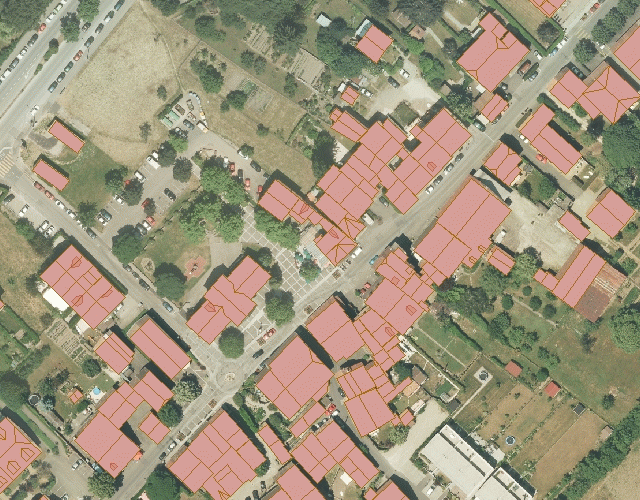
\includegraphics[width=1\linewidth]{02-main//figures/ch2/stdl_01_couche_vectorielle.png}
    \caption{Image d’exemple de la couche vectorielle d’emprise au sol des bâtiments ``CAD\_BATIMENTS\_HORSOL\_TOIT'' \cite{sitg_toits_nodate}}
    \label{fig:stdl_01_couche_vectorielle}
\end{figure}
\par{Cette couche est régulièrement mise à jour. \acrshort{stdl} a utilisé les données de mars 2023 pour son projet. Les superstructures sont des éléments qui dépassent de la toiture tel qu'une cheminée, cage d'ascenseur, lucarne, etc. ne sont pas représentés dans cette couche. Tout ce qui est en dessous de 9 m² ne figure pas dans cette couche.}

\paragraph{Vérité terrain}
\par{La Figure \ref{fig:stdl_02_verite_terrain} représente les bâtiments choisis par \acrshort{stdl} pour la vérité terrain.}
\begin{figure}[H]
    \centering
    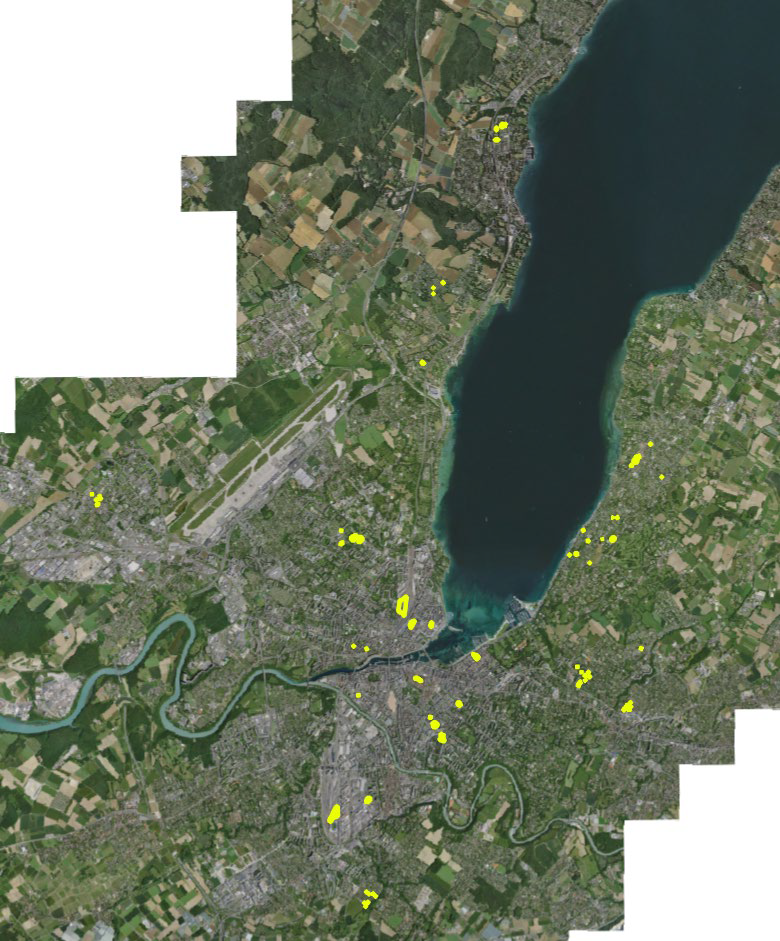
\includegraphics[width=1\linewidth]{02-main//figures/ch2/stdl_02_verite_terrain.png}
    \caption{Bâtiments choisis par STDL pour la vérité terrain dans le Canton de Genève. Images de \acrshort{sitg}}
    \label{fig:stdl_02_verite_terrain}
\end{figure}
\par{Ces bâtiments se distribuent de la manière suivante :}
\begin{itemize}
    \item 7 bâtiments administratifs (toiture plate)
    \item 18 bâtiments industriels (toiture plate)
    \item 97 bâtiments de logement (toiture en pente/plate)
\end{itemize}
\par{Les données ont été labellisées selon les classes suivantes :}
\begin{figure}[H]
    \centering
    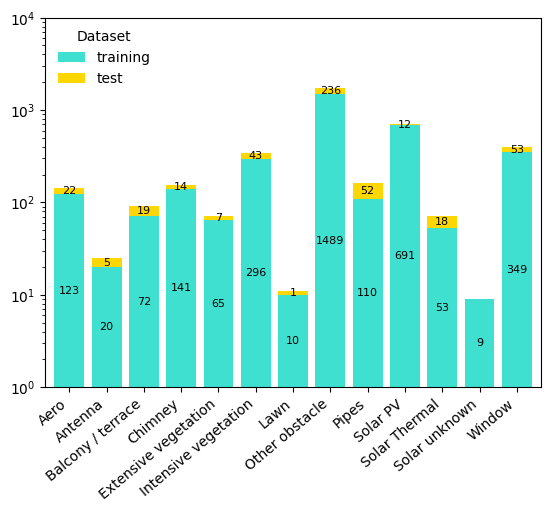
\includegraphics[width=1\linewidth]{02-main//figures/ch2/stdl_03_classes.png}
    \caption{Classes et répartition des datasets}
    \label{fig:stdl_03_classes}
\end{figure}
\par{Chaque méthode utilisée dans ce projet nécessite la création de vérité terrain spécifique.}

\subsubsection{Classification des pans de toits}
\par{Cette méthode consiste à utiliser les données vectorielles de l'emprise des toitures, les labelliser à l'aide des données \gls{lidar} et ensuite appliquer un algorithme random forest (similaire a un arbre de décision).}

\paragraph{Données}
\par{Les données utilisées sont la couche vectorielle de l'emprise des toitures, ainsi que les données \gls{lidar}.}
\par{Comme indiqué au chapitre ``XXXXXX'', la rugosité et l'intensité sont deux informations complémentaires fournies par les nuages de points \gls{lidar}. La rugosité mesure la variation locale de l'altitude des points et reflète la texture de la surface. Une rugosité élevée indique la présence d'obstacles. L'intensité mesure la quantité d'énergie réfléchie par la surface et dépend des propriétés de réflectance des matériaux. Elle varie selon le type de surface et peut aider à distinguer différents matériaux.}
\todo[inline]{Ajouter ici le lien correct aux annexes}
\par{Pour constituer le dataset (vérité terrain), \acrshort{stdl} a annoté la couche vectorielle de l'emprise des toitures avec l'aide des données \gls{lidar}. Les 3 classes résultantes sont :}
\begin{itemize}
    \item Occupé : pas de surface disponible
    \item Possiblement libre : probablement libre
    \item Non défini : le nuage de point \gls{lidar} n'a pas classifié cette zone comme ``bâtiment''
\end{itemize}

\paragraph{Méthodologie}
\par{La méthodologie se décompose en trois étapes principales : la préparation des données \gls{lidar}, la classification par seuils manuels et la classification par forêt aléatoire (random forest).}
\par{La première étape est la préparation des données \gls{lidar} :}
\begin{itemize}
    \item L'intensité du signal \gls{lidar} est interpolée par une méthode de pondération inverse à la distance pour obtenir une valeur continue en chaque point.
    \item Un modèle numérique de terrain (\acrshort{mnt}) est généré à partir des points \gls{lidar} pour représenter la surface du sol.
    \item La rugosité de la surface est calculée à partir du \acrshort{mnt} à une échelle de 1 m pour caractériser les variations locales de hauteur.
    \item Des statistiques zonales (moyenne, médiane, écart-type, etc.) sont calculées pour l'intensité et la rugosité sur chaque pan de toit.
\end{itemize}
\par{La deuxième étape est la classification par seuils manuels :}
\begin{itemize}
    \item Les pans de toit de moins de 2 m² sont automatiquement classés comme "occupés" car trop petits pour des installations.
    \item Les pans avec moins de 25\% de points classés comme "bâtiment" (données \gls{lidar}) sont classés en "non défini" par manque d'information.
    \item Pour les autres pans
    \begin{itemize}
        \item Des seuils sont fixés empiriquement sur 4 variables :
        \begin{itemize}
            \item La marge d'erreur et l'écart-type de l'intensité
            \item La rugosité médiane
            \item Le pourcentage de recouvrement avec des pixels non classés comme "bâtiment" (données \gls{lidar})
        \end{itemize}
        \item Si un pan dépasse le seuil pour au moins une variable, il est classé comme "occupé", sinon il est "potentiellement libre".
    \end{itemize}
    \item Cette classification est validée manuellement par des experts sur un échantillon de 650 pans de toit.
\end{itemize}
\par{La troisième étape est la classification par random forrest (RF)}
\begin{itemize}
    \item Deux forêts aléatoires sont entraînées, une pour chaque office (\acrshort{ocen} et \acrshort{ocan}), en utilisant les seuils validés comme référence.
    \item Les données sont divisées en 80\% pour l'entraînement et 20\% pour le test.
    \item 14 variables sont utilisées pour construire les arbres de décision, dont les statistiques zonales d'intensité et de rugosité.
    \item L'importance relative de chaque variable dans la classification est calculée.
    \item Les forêts sont évaluées sur l'échantillon test pour mesurer leur performance.
\end{itemize}

\paragraph{Résultats}
\par{Les résultats obtenus sont détaillés dans le Tableau \ref{tab:stdl_01_resultats_classification} :}
\begin{table}[h]
    \centering
    \begin{tabular}{|l|c|c|c||c|c|c|}
    \hline
    \multirow{2}{*}{} & \multicolumn{3}{c||}{Manual threshold classification} & \multicolumn{3}{c|}{RF classification} \\
    \cline{2-7}
    & Global & Occupied & Potentially free & Global & Occupied & Potentially free \\
    \hline
    OCAN & 79\% & 70\% & 91\% & 86\% & 78\% & 96\% \\
    OCEN & 77\% & 72\% & 82\% & 83\% & 74\% & 91\% \\
    \hline
    \end{tabular}
    \caption{Résultats obtenus par les deux algorithmes de classification}
    \label{tab:stdl_01_resultats_classification}
\end{table}
\par{La classification avec RF est plus performante que les seuils manuels, avec des taux de satisfaction augmentant de 7 et 6 points pour \acrshort{ocan} et \acrshort{ocen} respectivement.}

\par{La Figure \ref{fig:stdl_04_rf_resultats} présente un aperçu des résultats obtenus :}
\begin{figure}[H]
    \centering
    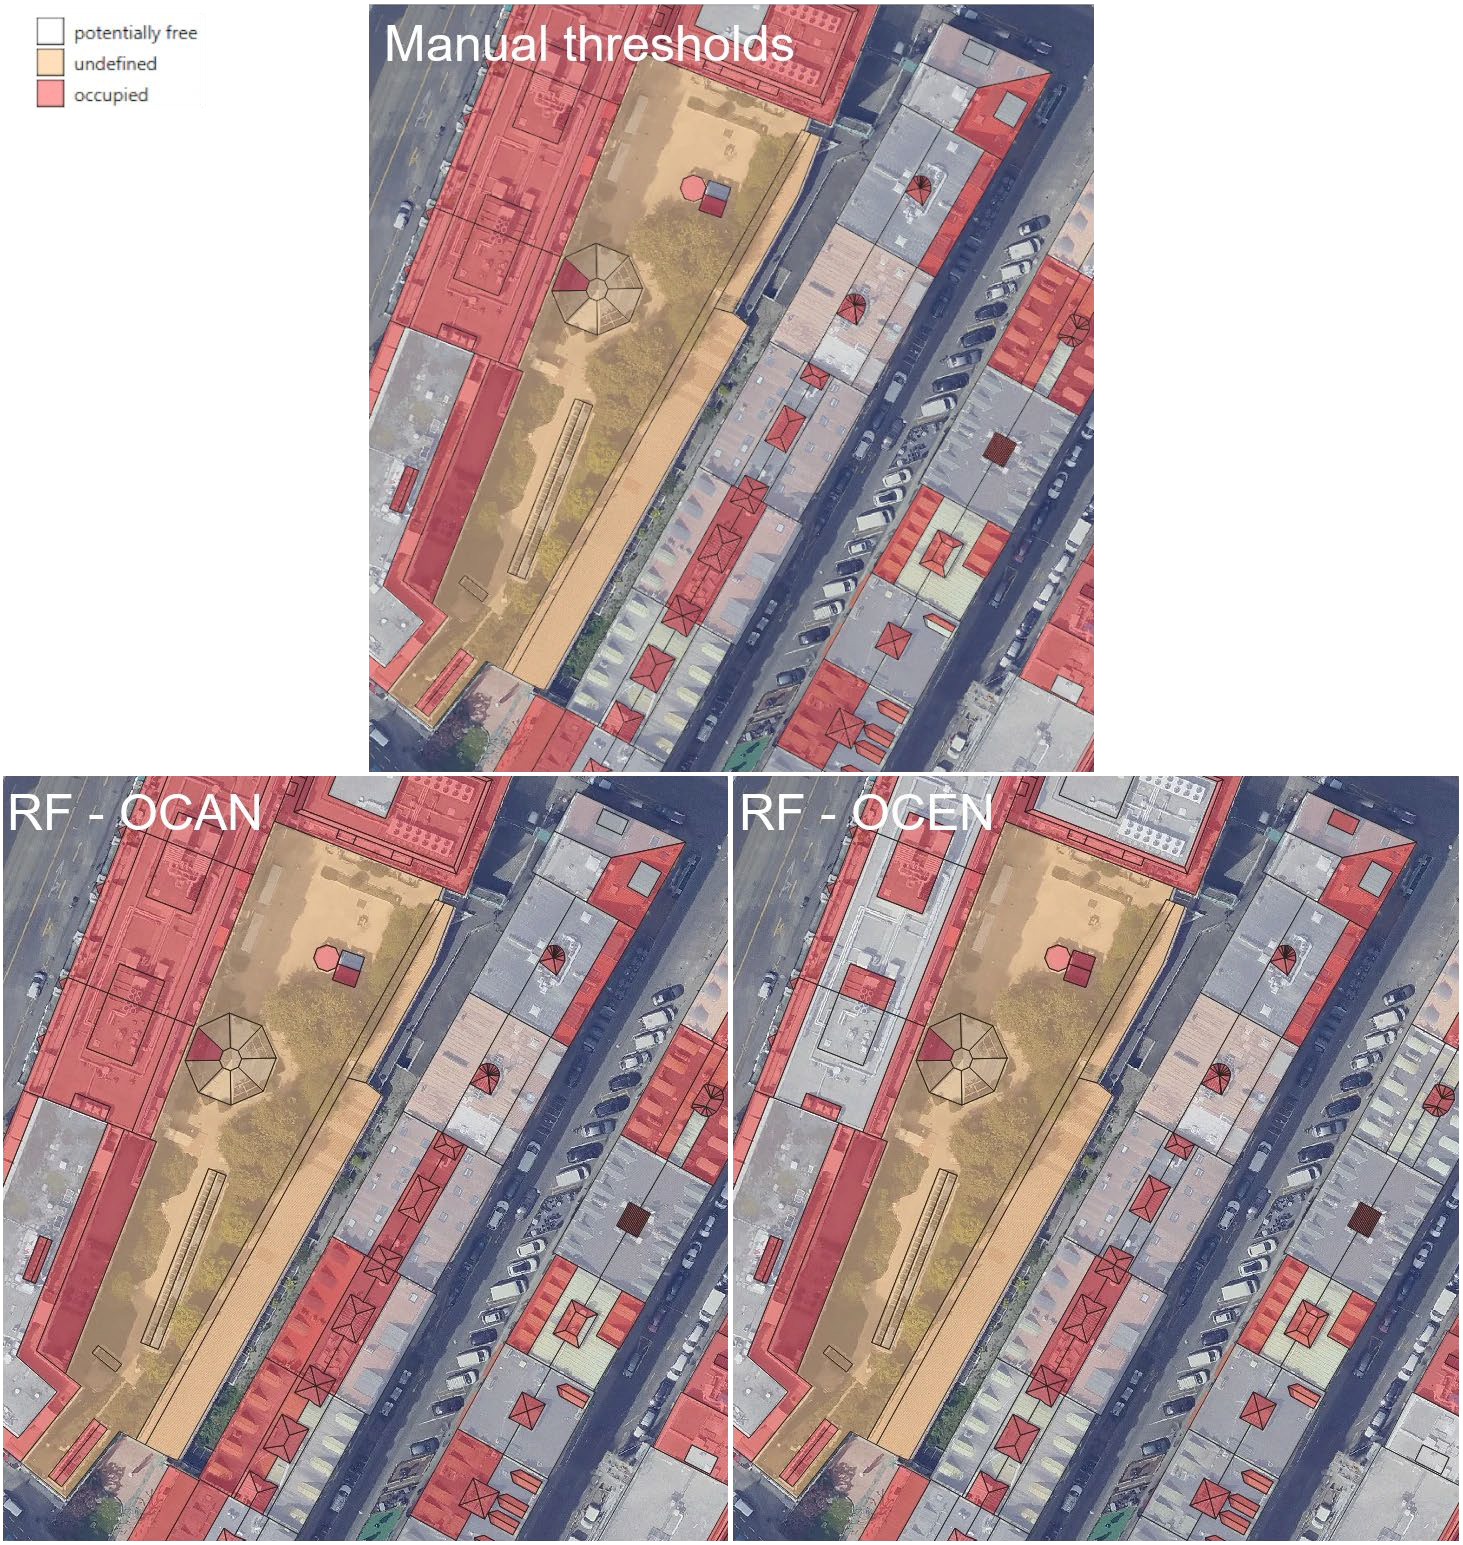
\includegraphics[width=1\linewidth]{02-main//figures/ch2/stdl_04_rf_resultats.png}
    \caption{Comparatif des différents algorithmes de classification \cite{herny_detection_2024}}
    \label{fig:stdl_04_rf_resultats}
\end{figure}
\par{Dans la Figure \ref{fig:stdl_04_rf_resultats} on observe les différents critères par office, l'\acrshort{ocen} semble classifier plus de surfaces comme ``possiblement libre'' (blanc) que l'\acrshort{ocan}. Une matrice de confiance aurait permis de mieux évaluer les résultats.}

\paragraph{Discussion des résultats (\acrshort{stdl})}
\par{Dans son rapport \acrshort{stdl} fait une analyse des résultats obtenus dans lequel ils traitent les points suivants :}
\begin{itemize}
    \item Comparaison des deux méthodes de classification
    \item Classification des petits pans de toit
    \item Différences entre les deux random forrest
    \item Pertinence de la méthodologie
\end{itemize}
\par{Le premier point soulevé est une comparaison de la classification par seuils et celle avec la random forrest :}
\begin{itemize}
    \item Les deux méthodes donnent des résultats satisfaisants, mais la forêt aléatoire est plus performante.
    \item La forêt aléatoire utilise 14 variables, contre seulement 4 pour les seuils manuels.
    \item Le choix des variables pour les seuils manuels était pertinent mais incomplet.
    \item Les seuils manuels sont simples à mettre en place mais nécessitent des tests manuels fastidieux.
    \item La forêt aléatoire est automatisée mais a besoin d'une vérité terrain.
\end{itemize}
\par{Le deuxième point est la classification des petits pans de toit :}
\begin{itemize}
    \item Avec les seuils manuels, les petits pans sont souvent classés comme "occupés" à cause de leur rugosité médiane élevée.
    \item La rugosité des petits pans est plus influencée par leur environnement à cause de l'échelle de calcul (1 m).
    \item La rugosité minimale, importante dans la forêt aléatoire, dépend fortement de la taille du pan.
    \item Bien que potentiellement utilisables, les petits pans dégagés sont difficiles à exploiter et moins prioritaires.
    \item Le fait que l'algorithme les classe souvent comme occupés convient aux experts.
\end{itemize}

\par{Le troisième point traite des raisons des différences entre les deux random forrest (une par office) :}
\begin{itemize}
    \item Les différences de résultats entre les offices (\acrshort{ocan} et \acrshort{ocen}) s'expliquent par leurs besoins distincts.
    \item Pour l'\acrshort{ocan} (végétalisation), une rugosité médiane élevée est tolérée.
    \item Pour l'\acrshort{ocen} (solaire), une grande surface continue et une faible rugosité minimale sont requises.
\end{itemize}

\par{Le quatrième point est la pertinence de la méthodologie utilisée :}
\begin{itemize}
    \item Les surfaces "potentiellement libres" doivent être examinées plus en détail.
    \item Les surfaces "occupées" sont considérées comme inutilisables.
    \item Les experts sont satisfaits des résultats obtenus.
    \item Il est prévu d'appliquer la méthode à plus grande échelle.
    \item La classification n'évalue que l'occupation, sans considérer la pente ou le matériau.
    \item L'intensité \gls{lidar} peut varier entre les acquisitions, affectant potentiellement les résultats.
\end{itemize}

\subsubsection{Segmentation \gls{lidar}}

\paragraph{Données}
\par{Les données utilisées sont des nuages de points \gls{lidar}, qui fournissent une représentation 3D précise des surfaces de toiture. Les toits sont délimités à partir d'une couche vectorielle existante, produite manuellement pour garantir sa qualité. Les points \gls{lidar} sont filtrés pour ne conserver que ceux situés au-dessus de l'altitude minimale de chaque toit.}

\paragraph{Méthodologie}
\par{La méthode proposée vise à détecter automatiquement les objets présents sur les toits, en supposant que chaque pan de toit peut être approximé par un plan et que les obstacles en dépassent. Le processus se déroule en plusieurs étapes :}
\begin{enumerate}
    \item Segmentation des plans de toit dans le nuage de points 3D à l'aide de l'algorithme RANSAC (RANdom SAmple Consensus), qui permet d'identifier les plans dominants.
    \item Application de l'algorithme DBSCAN (Density-Based Spatial Clustering of Applications with Noise) sur les points de chaque plan potentiel pour éliminer le bruit et ne retenir que le plus grand cluster.
    \item Considération des points restants comme des obstacles, regroupés à nouveau avec DBSCAN.
    \item Transformation des clusters de points en polygones concaves à l'aide de l'algorithme ``alpha shape'', en appliquant des seuils sur leur surface projetée pour distinguer les plans des obstacles.
    \item Optimisation des hyperparamètres des algorithmes RANSAC et DBSCAN, ainsi que des seuils de surface, sur un jeu de données d'entraînement, en tenant compte du type de bâtiment et de toit.
    \item Post-traitement des polygones détectés par lissage et fusion pour améliorer leur aspect visuel et créer une partition des surfaces occupées et libres sur chaque toit.
\end{enumerate}

\newpage
\paragraph{Résultats}
\par{Les experts de l'\acrshort{ocen} et l'\acrshort{ocan} n'ont pas apprécié les images résultantes (Figure \ref{fig:stdl_05_exemple_segmentation_lidar}) car ils s'attendaient à des polygones plus semblables aux couches vectorielles (par exemple Figure \ref{fig:stdl_01_couche_vectorielle}). \acrshort{stdl} a pourtant bien simplifié les polygones pour améliorer leur rendu visuel.}
\begin{figure}[H]
    \centering
    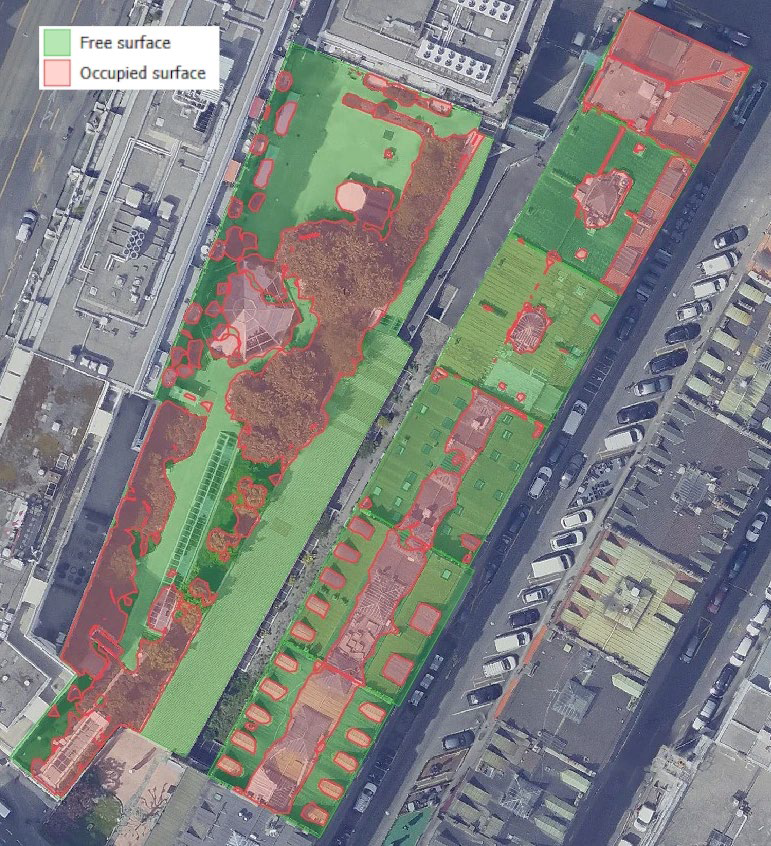
\includegraphics[width=1\linewidth]{02-main//figures/ch2/stdl_05_exemple_segmentation_lidar.png}
    \caption{Image d’exemple de la segmentation \gls{lidar} \cite{herny_detection_2024}}
    \label{fig:stdl_05_exemple_segmentation_lidar}
\end{figure}
\newpage
\par{L'algorithme obtient un F1-score de 0.77 et un mIoU (mean Intersection over Union) de 0.38 sur l'ensemble des données de test. Le Tableau \ref{tab:stdl_02_resultats_segmentation_lidar} ci-dessous résume les principales métriques obtenues.}
\begin{table}[H]
    \centering
    \begin{tabular}{|l|c|c|c|c|c|}
    \hline
    Ground truth & Precision & Recall & f1 score & mIoU & Relative error (\%) \\
    \hline
    adapted GT, training set & 0.77 & 0.77 & 0.77 & 0.42 & 11 \\
    whole GT, training set & 0.78 & 0.77 & 0.78 & 0.35 & 38 \\
    whole GT, test set & 0.75 & 0.80 & 0.77 & 0.38 & 26 \\
    \hline
    \end{tabular}
    \caption{Métriques obtenus par la segmentation \gls{lidar}}
    \label{tab:stdl_02_resultats_segmentation_lidar}
\end{table}

\par{Les objets de plus de 1 m² (Figure \ref{fig:stdl_06_segmentation_lidar_surfaces}) et situés à plus de 1 m (Figure \ref{fig:stdl_07_segmentation_lidar_distances}) du bord du toit sont bien détectés, avec des F1-score entre 0.82 et 0.92.}
\begin{figure}[H]
    \centering
    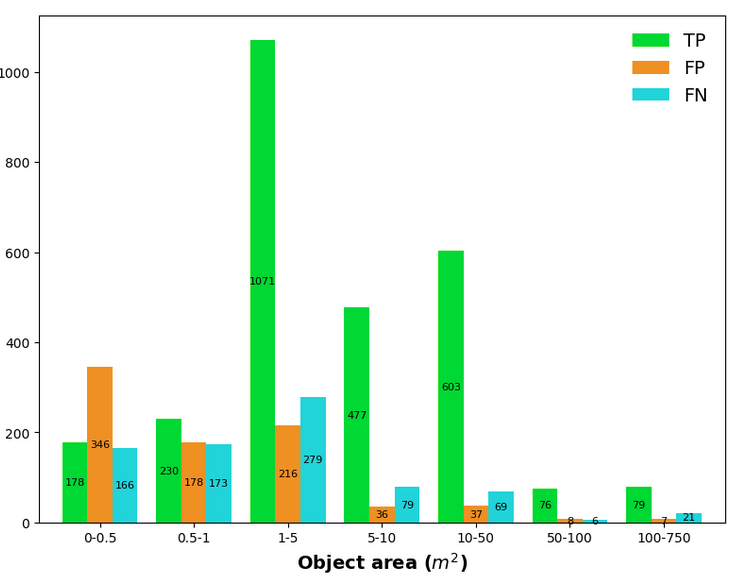
\includegraphics[width=1\linewidth]{02-main//figures/ch2/stdl_06_segmentation_lidar_surfaces.png}
    \caption{Influence de la distance des objets au bord du toit selon la surface de l’objet dans la segmentation \gls{lidar} \cite{herny_detection_2024}}
    \label{fig:stdl_06_segmentation_lidar_surfaces}
\end{figure}
\newpage
\par{Les objets (Figure \ref{fig:stdl_07_segmentation_lidar_distances}) qui ont leur centroïde a plus d'un mètre du bord du toit sont bien labellisés. Le F1-score est entre 0.80 et 0.85 pour ces objets. Cependant, les objets qui ont leur centroïde proche du bord (moins d'un mètre) ne sont pas bien détectés et ont 65\% de faux positif (FP), ce qui indique que la segmentation n'est pas fiable à cette distance.}

\begin{figure}[H]
    \centering
    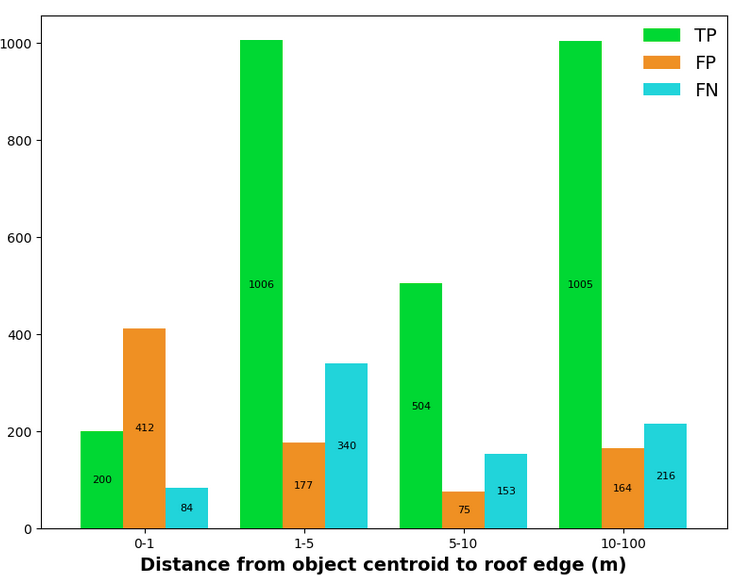
\includegraphics[width=1\linewidth]{02-main//figures/ch2/stdl_07_segmentation_lidar_distances.png}
    \caption{Influence de la distance du centre des objets au bord du toit dans la segmentation \gls{lidar} \cite{herny_detection_2024}}
    \label{fig:stdl_07_segmentation_lidar_distances}
\end{figure}
\newpage
\par{La plupart (Tableau \ref{tab:stdl_03_resultats_segmentation_lidar_classes}) des classes d'objets (bouches d'aération, balcons, végétation intensive, panneaux solaires) ont des recalls supérieurs à 0.80. Cependant, les antennes et les objets bas (fenêtres, végétation extensive, pelouses) sont plus difficiles à détecter.}

\begin{table}[H]
    \centering
    \begin{tabular}{|l|c|}
    \hline
    Object class & Recall \\
    \hline
    Antenna & 0.24 \\
    Pipe & 0.59 \\
    Lawn & 0.70 \\
    Other obstacle & 0.70 \\
    Extensive vegetation & 0.72 \\
    Window & 0.76 \\
    Chimney & 0.79 \\
    Aero & 0.83 \\
    Solar thermal & 0.83 \\
    Intensive vegetation & 0.88 \\
    Solar unknown & 0.89 \\
    Balcony / terrace & 0.90 \\
    Solar photovoltaic & 0.92 \\
    \hline
    \end{tabular}
    \caption{Recall par classe pour la segmentation LiDAR (STDL, 2024)}
    \label{tab:stdl_03_resultats_segmentation_lidar_classes}
\end{table}

\par{La surface occupée (Tableau \ref{tab:stdl_04_resultats_segmentation_lidar_affectation}) totale est sous-estimée de 38\% par rapport à la vérité terrain.}

\begin{table}[H]
    \centering
    \begin{tabular}{|p{2.7cm}|c|c|c|c|c|c|}
    \hline
    & Administrative & Industrial & Residential & Flat & Mixed & Pitched \\
    \hline
    Area labeled as occupied & 4,986 & 32,720 & 19,399 & 54,875 & 1,386 & 844 \\
    Area detected as occupied & 1,195 & 20,953 & 12,986 & 30,980 & 3,052 & 1,102 \\
    Detection rate (\%) & 24\% & 64\% & 67\% & 56\% & 220\% & 131\% \\
    Total area & 6,692 & 78,011 & 33,278 & 108,415 & 5,018 & 4,584 \\
    \hline
    \end{tabular}
    \caption{Récapitulatif des surfaces détectées et vérité terrain pour la segmentation \gls{lidar}}
    \label{tab:stdl_04_resultats_segmentation_lidar_affectation}
\end{table}


\newpage
\par{Les experts (Tableau \ref{tab:stdl_05_resultats_segmentation_lidar_experts}) sont au moins partiellement satisfaits par plus de 69\% des toits segmentés.}

\begin{table}[H]
    \centering
    \begin{tabular}{|l|c|c|}
    \hline
    Evaluation & OCAN & OCEN \\
    \hline
    Not satisfied & 22\% & 31\% \\
    Partially satisfied & 54\% & 33\% \\
    Satisfied & 24\% & 36\% \\
    \hline
    \end{tabular}
    \caption{Evaluation des experts pour la segmentation \gls{lidar}}
    \label{tab:stdl_05_resultats_segmentation_lidar_experts}
\end{table}

\paragraph{Discussion des résultats (\acrshort{stdl})}
\par{La méthode prouve sa capacité à détecter les objets sur les toits, en particulier ceux de grande taille et éloignés des bords. Cependant, la délimitation précise des formes reste perfectible, comme en témoigne le faible mIoU. L'estimation de la surface occupée est moyenne, avec une erreur importante liée à la sous-détection des objets bas. Les faux positifs sont souvent de petite taille et situés près des bords, parfois à cause de l'absence de barrières dans la vérité terrain.}
\par{Les bâtiments administratifs et les toits en pente posent des difficultés spécifiques, nécessitant des hyperparamètres adaptés.}
\par{Malgré des résultats honorables, l'aspect visuel des détections reste à améliorer pour une utilisation opérationnelle par les experts. Des développements futurs pourraient inclure l'automatisation de la production de la couche vectorielle des toits et l'ajustement de formes géométriques simples sur les clusters de points pour obtenir des détections plus précises et esthétiques.}

\newpage
\subsubsection{Segmentation d'image}

\paragraph{Données}

\par{Les données utilisées sont :}
\begin{itemize}
    \item True orthophotos \cite{sitg_orthophotos_nodate}
    \item Couche vectorielle des toitures modifiée comme pour la segmentation \gls{lidar}
\end{itemize}

\paragraph{Méthodologie}
La Figure \ref{fig:stdl_08_methodo_segmentation_images} ci-dessous représente les principales étapes utilisées pour réaliser la segmentation d'image.
\begin{figure}[H]
    \centering
    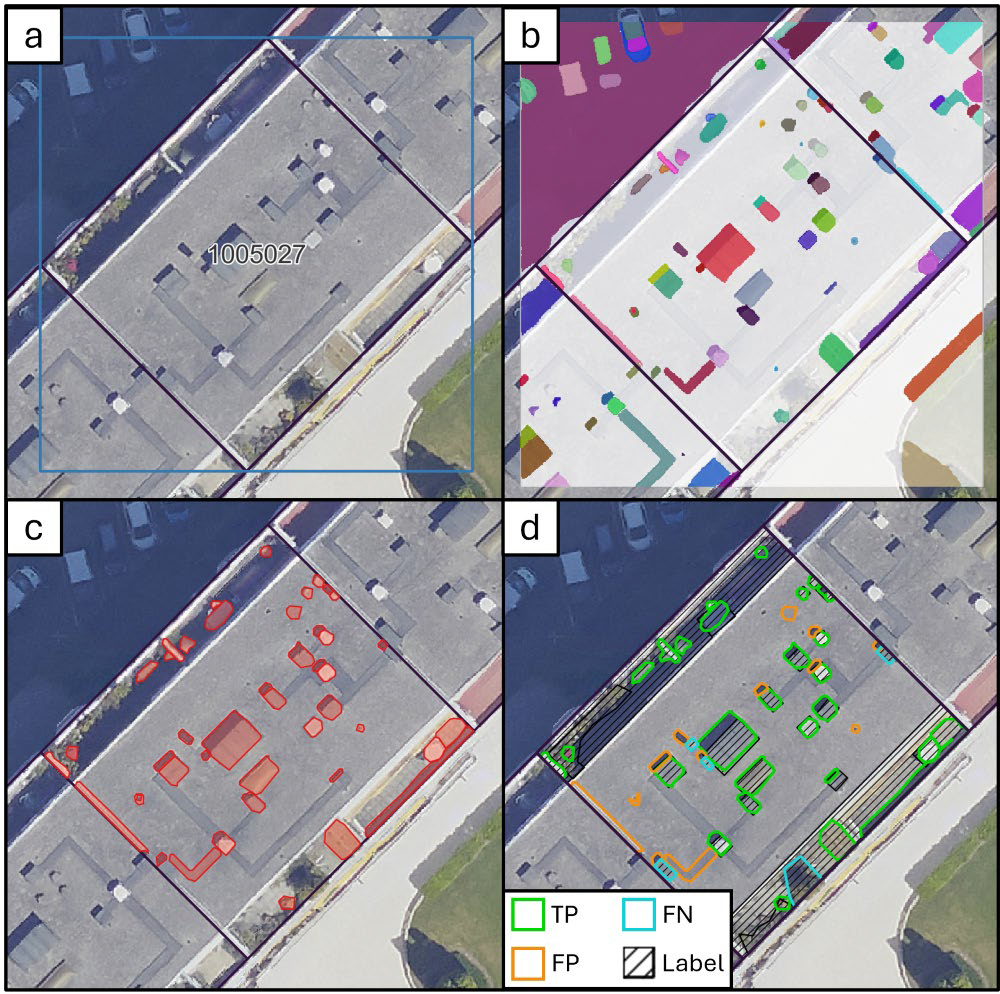
\includegraphics[width=1\linewidth]{02-main//figures/ch2/stdl_08_methodo_segmentation_images.png}
    \caption{Méthodologie pour la segmentation d’images \cite{herny_detection_2024}}
    \label{fig:stdl_08_methodo_segmentation_images}
\end{figure}

\par{La première étape est la préparation des orthophotos (Figure \ref{fig:stdl_08_methodo_segmentation_images} ``a''). Celle-ci commence par le découpage des orthophotos avec les données vectorielles des toitures (délimitation des toitures) pour ne conserver que la toiture à segmenter. La ligne bleue représente la marge de 1 mètre (zone tampon) pour faciliter la tâche de l'algorithme. Ensuite chaque toiture fera l'objet d'une tuile (une toiture par image).}

\par{La deuxième étape est la segmentation de l'image (Figure \ref{fig:stdl_08_methodo_segmentation_images} ``b''). Le modèle segment anything model (SAM) est utilisé via la librairie Python ``segment-geospatial'' \cite{wu_samgeo_2023} car cette libraire permet d'utiliser SAM sur des orthophotos tout en conservant les données géospatiales. SAM va segmenter les objets sur la toiture dans chaque tuile, ce qui va produire un masque par objet segmenté.}

\par{La troisième étape est la vectorisation des objets (Figure \ref{fig:stdl_08_methodo_segmentation_images} ``c''). Dans cette étape, les masques segmentés sont convertis en données vectorielles. Certains de ces polygones sont supprimés basé sur des critères géométriques :}
\begin{itemize}
    \item Polygone de moins de 0.2 m²
    \item Polygones qui occupent plus de 90\% de la surface de la toiture
    \item Polygones qui ont une surface de plus de 50\% de la toiture et qui n'ont pas d'intersection avec la toiture
\end{itemize}

\par{La quatrième étape est l'optimisation des hyperparamètres (Figure \ref{fig:stdl_08_methodo_segmentation_images} ``d'') de SAM et l'évaluation de ses résultats avec la vérité terrain.}

\par{La logique est que tout ce qui n'est pas segmenté à l'intérieur du périmètre de la toiture est une surface libre.}

\newpage
\paragraph{Résultats}

\par{La Figure \ref{fig:stdl_09_segmentation_image_resultats} représente un exemple de résultat de la segmentation de plusieurs toitures. On peut observer que la segmentation rencontre des difficultés avec certains éléments de toiture tel que les puits de lumière.}
\begin{figure}[H]
    \centering
    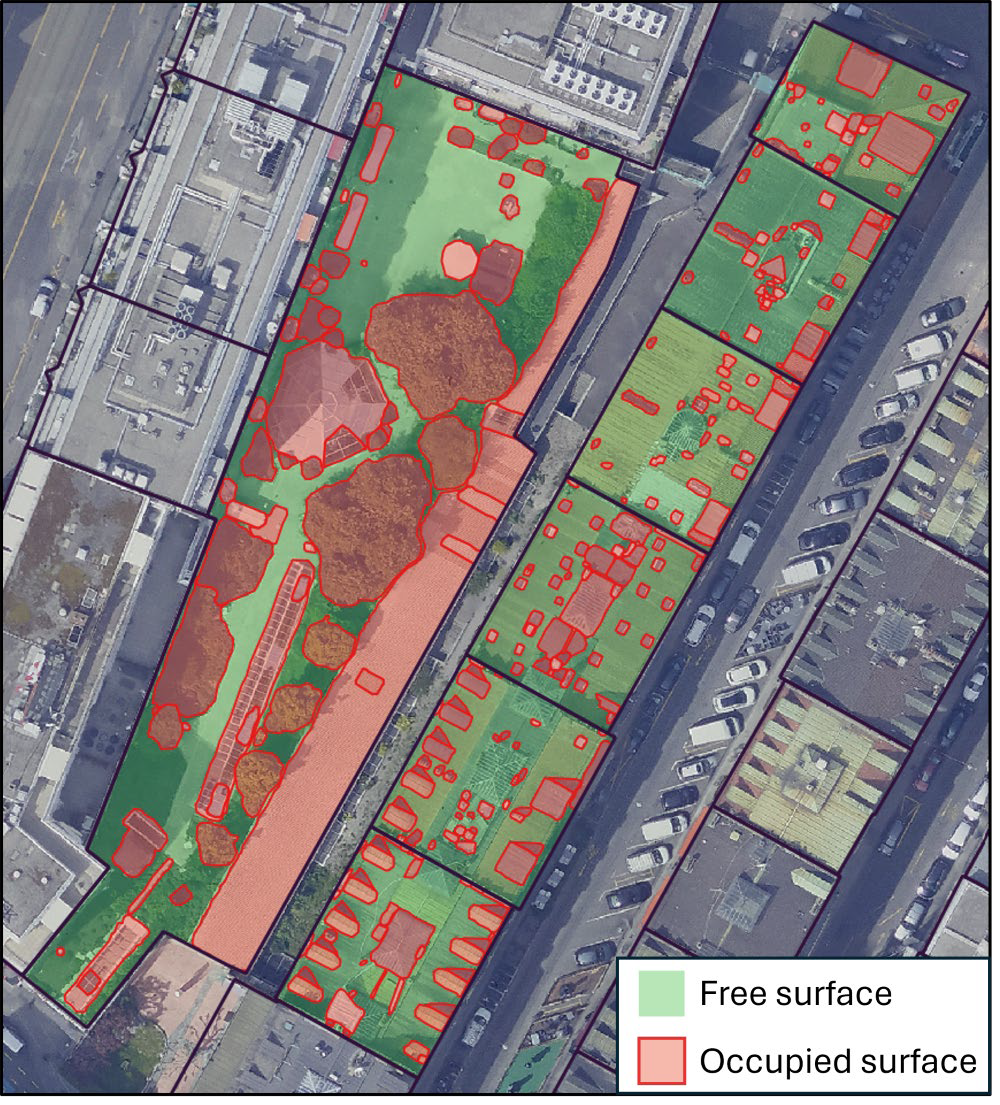
\includegraphics[width=1\linewidth]{02-main//figures/ch2/stdl_09_segmentation_image_resultats.png}
    \caption{Exemple d’image résultat de la segmentation d’images \cite{herny_detection_2024}}
    \label{fig:stdl_09_segmentation_image_resultats}
\end{figure}
\newpage
\par{Les métriques obtenues (Tableau \ref{tab:stdl_06_segmentation_image_resultats}) sur le dataset de test sont un F1-score de 0.73 et mIoU de 0.37.}
\begin{table}[H]
    \centering
    \begin{tabular}{|l|c|c|c|c|c|}
    \hline
    Dataset & Precision & Recall & f1 score & mIoU & Relative error (\%) \\
    \hline
    Training subset & 0.73 & 0.78 & 0.75 & 0.41 & 7 \\
    Training & 0.75 & 0.82 & 0.78 & 0.37 & 42 \\
    Test & 0.75 & 0.71 & 0.73 & 0.37 & 23 \\
    \hline
    \end{tabular}
    \caption{Métriques obtenues par la segmentation d'images}
    \label{tab:stdl_06_segmentation_image_resultats}
\end{table}
\par{Les petits objets (Figure \ref{fig:stdl_10_segmentation_image_taille}) avec une surface de moins d'un mètre carré sont moins bien détectés (AP d'environ 0.60). Les objets de plus d'un mètre carré sont mieux détectés (AP d'environ 0.83).}
\begin{figure}[H]
    \centering
    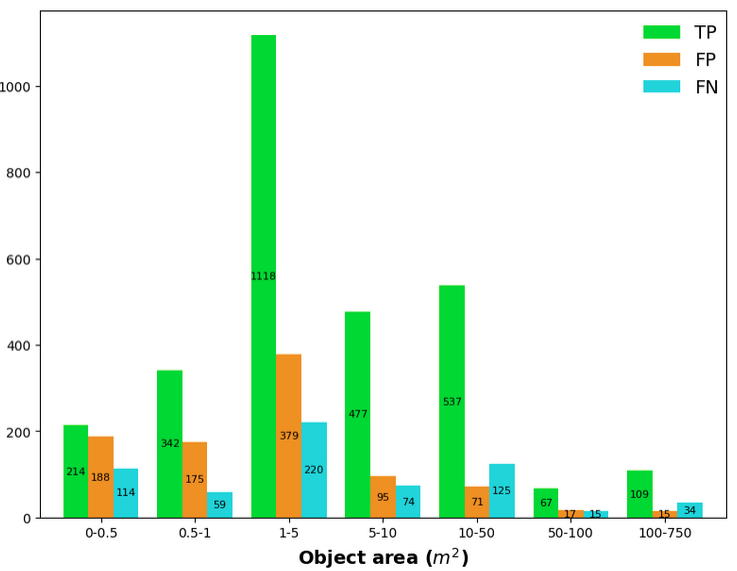
\includegraphics[width=1\linewidth]{02-main//figures/ch2/stdl_10_segmentation_image_taille.png}
    \caption{Objets segmentés selon taille en m² pour la segmentation d’images \cite{herny_detection_2024}}
    \label{fig:stdl_10_segmentation_image_taille}
\end{figure}
\newpage
\par{Comme pour la segmentation \gls{lidar}, la segmentation d'image fonctionne moins bien au bord de la toiture (Figure \ref{fig:stdl_11_segmentation_image_distance}). La precision est de 0.77 pour les centroïde d'objets a plus d'un mètre du bord de la toiture contre seulement 0.51 pour ceux a moins d'un mètre.}

\begin{figure}[H]
    \centering
    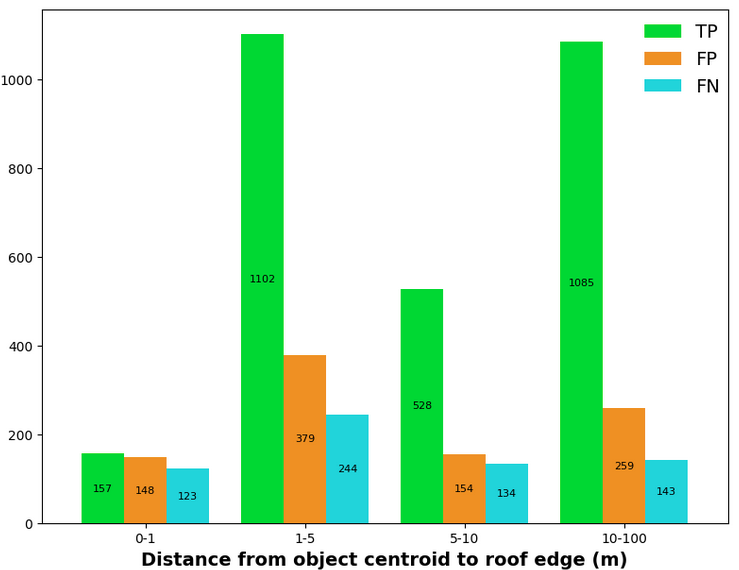
\includegraphics[width=1\linewidth]{02-main//figures/ch2/stdl_11_segmentation_image_distance.png}
    \caption{Centroïde des objets segmentés selon la distance au borde de la toiture pour la segmentation d’images  \cite{herny_detection_2024}}
    \label{fig:stdl_11_segmentation_image_distance}
\end{figure}

\par{Les experts sont au minimum partiellement satisfait de 86\% des résultats (Tableau .}
\begin{table}[h]
    \centering
    \begin{tabular}{|l|c|c|}
    \hline
    Evaluation & OCAN & OCEN \\
    \hline
    Not satisfied & 6\% & 14\% \\
    Partially satisfied & 40\% & 49\% \\
    Satisfied & 54\% & 37\% \\
    \hline
    \end{tabular}
    \caption{Evaluation des experts pour la segmentation d'images (STDL, 2024)}
    \label{tab:stdl_07_segmentation_image_resultats_experts}
\end{table}
\newpage
\paragraph{Discussion résultats (\acrshort{stdl})}

\par{Points forts de cette approche :}
\begin{itemize}
\item Bonne capacité générale à détecter et segmenter correctement les objets
\item Métriques cohérentes
\item Forme des objets détectés généralement bien reproduite
\end{itemize}

\par{Limites constatées de la méthodologie utilisée :}
\begin{itemize}
\item Difficulté à détecter les objets tel que les gaines ou d'autres petits objets
\item Sensibilité aux changements de couleurs (saleté, ombres, pans de toit) pouvant être interprétés comme des objets
\item Temps de calcul important (12 minutes pour 25 bâtiments), mise à l'échelle du canton (plus de 80'000 bâtiments) compliquée
\item Nécessité des true orthophotos, plus rares et coûteuses que les orthophotos standards
\end{itemize}

\par{Potentielles améliorations :}
\begin{itemize}
\item Fine-tuning du modèle SAM
\item Méthodes pour atténuer la présence d'ombres dans les images
\item Adaptation de la méthodologie pour utiliser des orthophotos standard
\end{itemize}

\subsubsection{Combinaison}

\par{Ce chapitre va traiter la combinaison des résultats de 2 méthodologies différentes pour améliorer les résultats finaux.}

\paragraph{Données}

\par{Les données utilisées sont le résultat des méthodologies de segmentation \gls{lidar} et celui de la segmentation d'images. Ce sont des données vectorielles.}

\paragraph{Méthodologie}

\par{Deux méthodes de combinaison des résultats ont été testées.}

\par{La première est la concaténation des objets détectés à partir des couches vectorielles produites par les segmentations \gls{lidar} et d'images.}

\par{La deuxième est la jointure spatiale des résultats de la segmentation \gls{lidar} et d'images. Dans ce cas, il faut :}
\begin{itemize}
    \item Sélectionner les polygones qui se chevauchent entre les couches vectorielles des segmentations \gls{lidar} et d'images.
    \item Conserver les polygones issus de la segmentation d'images car ils fournissent une meilleure délimitation
\end{itemize}
\newpage
\paragraph{Résultats}

\par{Les couches vectorielles obtenues n'ont pas été évaluées par les experts. Le Tableau \ref{tab:stdl_08_ensemble_resultats} ci-dessous résume les principales métriques obtenues.}

\begin{table}[H]
    \centering
    \begin{tabular}{|l|c|c|c|c|c|}
    \hline
    Combination method & Precision & Recall & f1 score & mIoU & Relative error (\%) \\
    \hline
    Concatenation & 0.68 & 0.94 & 0.79 & 0.45 & 8 \\
    Spatial join & 0.81 & 0.69 & 0.75 & 0.33 & 48 \\
    \hline
    \end{tabular}
    \caption{Métriques obtenues par les méthodes de combinaison}
    \label{tab:stdl_08_ensemble_resultats}
\end{table}

\par{En complément du Tableau \ref{tab:stdl_08_ensemble_resultats}, le Tableau \ref{tab:stdl_09_resultats_methodos} récapitule l'ensemble des métriques des méthodologies. La méthodologie de classification des pans de toit n'a pas de métrique, elle n'est donc pas incluse dans le tableau.}

\begin{table}[H]
    \centering
    \begin{tabular}{|l|c|c|c|c|c|}
    \hline
    Méthodologie & Precision & Recall & F1-score & mIoU & Relative error [\%] \\
    \hline
    Segmentation \gls{lidar} & 0.75 & 0.80 & 0.77 & 0.38 & 26 \\
    Segmentation d'image & 0.75 & 0.71 & 0.73 & 0.37 & 23 \\
    Concaténation & 0.68 & 0.94 & 0.79 & 0.45 & 8 \\
    Jointure spatiale & 0.81 & 0.69 & 0.75 & 0.33 & 48 \\
    \hline
    \end{tabular}
    \caption{Comparatif des résultats des différentes méthodologies}
    \label{tab:stdl_09_resultats_methodos}
\end{table}

\par{Les F1-scores des deux méthodes de combinaison sont proches, autour de 0.77, ce qui suggère des performances globales similaires.}

\par{La concaténation obtient un recall exceptionnel de 0.94, détectant presque toutes les surfaces occupées. En contrepartie, la précision diminue d'environ 8 points, indiquant plus de faux positifs dans les résultats.}

\par{La jointure spatiale fait le choix inverse : elle améliore la précision de 6 points en réduisant les détections erronées, mais perd 8 points de recall, manquant davantage de surfaces réellement occupées.}

\par{Le mIoU favorise nettement la concaténation avec un gain de plus de 10 points, reflétant une segmentation de meilleure qualité. Cette tendance se confirme pour l'estimation des surfaces : la concaténation maintient l'erreur relative sous 10\% tandis que la jointure spatiale atteint environ 50\%.}

\paragraph{Discussion des résultats (\acrshort{stdl})}

Les points positifs de cette approche sont :
\begin{itemize}
    \item La combinaison des résultats permet de moduler les résultats en favorisant soit la précision soit le recall selon les besoins
    \item La valeur élevée du recall obtenue par concaténation prouve la complémentarité des deux méthodes pour détecter différents objets
\end{itemize}

\par{La valeur de recall élevée obtenue avec la concaténation prouve la complémentarité des deux méthodes pour la détection d'objets différents. Une valeur de recall plus élevée tend à favoriser le mIoU, puisque plus d'objets sont détectés (TP), malgré l'ajout de faux positifs (FP). La surface de l'objet détecté est donc améliorée, mais l'ajout de FP contribue également à la réduction de l'erreur relative sur la surface occupée, ce qui doit être analysé avec soin.}

\par{L'utilisation des couches vectorielles des toits et superstructures produites par l'État de Genève, bien qu'incomplètes, pourrait améliorer les résultats.}

\subsubsection{Conclusion}

\par{\acrshort{stdl} a exploré trois méthodes pour détecter les objets sur les toits à partir de données \gls{lidar}, d'orthophotos et vectorielles. Toutes les méthodes ont fourni des résultats satisfaisants, avec une précision de 85\% pour la classification d'occupation et un F1-score d'environ 0,77 pour les méthodes de segmentation. Les bénéficiaires ont été satisfaits des résultats dans au moins 70\% des cas.}

\par{La méthode de classification a été sélectionnée en raison de ses bonnes performances et résultats obtenus.}

\par{La combinaison des résultats de segmentation permet d'améliorer soit la précision, soit le recall, et le croisement des sources d'information peut améliorer la précision des résultats.}

\par{Il est important de noter que ces résultats sont des indications qui doivent être vérifiées par un expert métier. Des paramètres supplémentaires, tels que le matériau du toit et le potentiel solaire, ne sont pas pris en compte.}

\subsubsection{Analyse critique}

\paragraph{Général}

\par{Le projet étant encore dans sa phase initiale explorative, il ne tient pas compte de l'orientation des toitures pour évaluer le potentiel solaire de chacune d'entre elle. L'exposition au soleil est en effet un facteur essentiel pour la pose de panneaux solaire. L'exclusion de toitures sur la base des données du cadastre solaire pourrait éventuellement éviter de traiter les toitures à l'ombre.}

\par{La végétalisation de toitures impose des défis considérables d'un point de vue génie civil, en effet les toitures ne sont souvent pas prévues pour porter des charges tel que de la terre végétale. Même dans le cas des panneaux solaires, pas toutes les toitures peuvent supporter la charge. Par exemple une toiture en fibrociment (toiture typique des hangars) n'aura probablement pas la capacité pour accueillir des panneaux solaires, cela pourrait être un critère d'exclusion.}

\par{L'échantillon de bâtiments du dataset ne semble pas très équilibré entre les différentes classes \gls{sia} de bâtiments \cite{sia_sia-shop_nodate}. En effet, les piscines couvertes, écoles, dépôts, hôpitaux ont pas mal en commun en ce qui concerne les toitures, elles seront probablement plates avec des éléments de ventilation ou froid. Les logements collectifs sont probablement plus complexes à segmenter car en général les toitures sont déjà assez occupées.}

\paragraph{Classification des pans de toiture}

\par{Les données de la couche vectorielle d'emprise au sol des bâtiments ne donnent pas un aperçu complet de la toiture, en effet les superstructures se trouvent dans une autre couche vectorielle. Même si ce n'est pas mentionné, les deux couches ont probablement été fusionnées.}

\par{Dans le rapport de \acrshort{stdl}, il manque une matrice de confusion. Cela aurait permis d'avoir une meilleure appréciation des performances obtenues par les différentes variantes utilisées.}

\paragraph{Segmentation \gls{lidar}}

\par{Le choix d'utiliser les données \gls{lidar} de 2019 avec les orthophotos de 2019 est tout à fait logique. Des données \gls{lidar} plus récentes et avec plus de densité existent mais il n'y a pas de true orthophoto après 2019 qui servirait de vérité terrain. Cela enlèverait aussi la possibilité de comparer les différents modèles de segmentation sur des données similaires.}

\paragraph{Segmentation d'images}

\par{La stratégie utilisée pour la segmentation d'images est très futée. La stratégie est principalement :}
\begin{itemize}
    \item Segmentation avec SAM
    \item Enlever certains masques trop petits ou qui sont en dehors de la toiture
    \item Tout ce qui n'a pas de masque devient donc une surface disponible
\end{itemize}

\par{\acrshort{stdl} l'a déjà indiqué dans son rapport, après avoir expérimenté avec SAM, il est tout de même très sensible aux ombrages. L'approche fonctionne moyennement bien avec un mIoU de 0.37.}

\par{En revanche, la stratégie de faire une tuile par toiture semble compliquée et le temps nécessaire est relativement long (12 minutes pour 25 bâtiments).}

\par{La segmentation à l'aide d'un algorithme de machine learning supervisé semble plus pertinente, l'inférence d'une image prend moins d'une minute pour un modèle de type YOLO et celle-ci peut contenir plusieurs bâtiments.}

\paragraph{Combinaison des résultats}

\par{\acrshort{stdl} n'a pas inclus dans leur rapport un tableau qui récapitule les résultats des différentes méthodologies utilisées. C'est donc difficile d'avoir une idée des résultats globaux.}

\paragraph{Résultats}

\par{Le Tableau \ref{tab:stdl_09_resultats_methodos} permet d'avoir une vue d'ensemble des résultats et la concaténation est fort intéressante.}

\par{La concaténation des résultats des deux méthodes de segmentation (\gls{lidar} et image) permet d'obtenir un recall élevé, ce qui signifie que la grande majorité des objets présents dans la vérité terrain (GT) sont détectés. Ce recall élevé s'explique par le fait que les deux méthodes ont des forces complémentaires : chacune est capable de détecter des types d'objets différents que l'autre méthode peut manquer.}

\par{Par exemple, la segmentation d'image peut mieux détecter les objets fins et bas, tandis que la segmentation \gls{lidar} peut mieux gérer les changements de couleur et détecter les gaines.}

\par{Un recall plus élevé a tendance à améliorer la métrique mIoU (mean Intersection over Union), car davantage d'objets GT sont correctement détectés (vrais positifs, TP), même si cela s'accompagne également de l'ajout de faux positifs (FP). Le mIoU mesure la qualité de la segmentation en calculant le chevauchement moyen entre les objets détectés et les objets GT. Avec plus de TP, le numérateur du mIoU augmente, ce qui améliore le score global.}

\par{De plus, un recall élevé permet une meilleure estimation de la surface occupée par les objets détectés. Cependant, l'ajout de FP lors de la concaténation peut également contribuer à cette surface occupée, ce qui peut réduire artificiellement l'erreur relative par rapport à la surface occupée réelle (calculée à partir de la GT). Il est donc important d'interpréter ce résultat avec prudence, car une faible erreur relative sur la surface occupée ne signifie pas nécessairement que la segmentation est parfaite, mais peut être influencée par la présence de FP.}

% -----------------------------------------------------------------------------
\subsection{SolarNet plus}
\label{subsec:solar_net_plus}

\subsubsection{Contexte et objectifs}
\par{\citeauthor{li_deep_2024} présentent SolarNet+ \cite{li_deep_2024}, un framework basé sur l'apprentissage profond qui vise à estimer avec précision le potentiel solaire des toitures urbaines. Cet article est la suite de l'article \cite{li_solarnet_2023} SolarNet par les mêmes auteurs principaux}
\par{Contrairement aux méthodes existantes, SolarNet+ prend en compte simultanément l'orientation des toits et les superstructures présentes (cheminées, fenêtres, etc.) qui réduisent la surface disponible pour l'installation de panneaux solaires. Cette approche permet d'éviter une surestimation du potentiel solaire et offre une évaluation plus précise pour soutenir la planification énergétique durable et les objectifs de neutralité carbone.}

\subsubsection{Données}
\par{L'étude utilise principalement le jeu de données RID (Roof Information Dataset). Le dataset est décrit en détail dans la sous-section \ref{subsec:rid_roof_information_dataset}.}
\par{Le dataset consiste en 1880 images satellite en provenance de google. Les images disposent des annotations suivantes:
\begin{itemize}
    \item Les segments de toiture et leur orientation (plat, N, E, S, W)
    \item Éléments de toiture
    \begin{itemize}
        \item Panneau PV
        \item Lucarne
        \item Fenêtre
        \item Échelle
        \item Cheminée
        \item Ombrage
        \item Arbre/végétation
        \item Fond d'image (background)
        \item Inconnu
    \end{itemize}
\end{itemize}}
\par{La Figure \ref{fig:rid_dataset_sample} représente une image d'exemple ainsi que ses annotations. Le jeu de données est divisé en dataset d'entraînement (70\%), de validation (10\%) et de test (20\%).}
\begin{figure}[H]
    \centering
        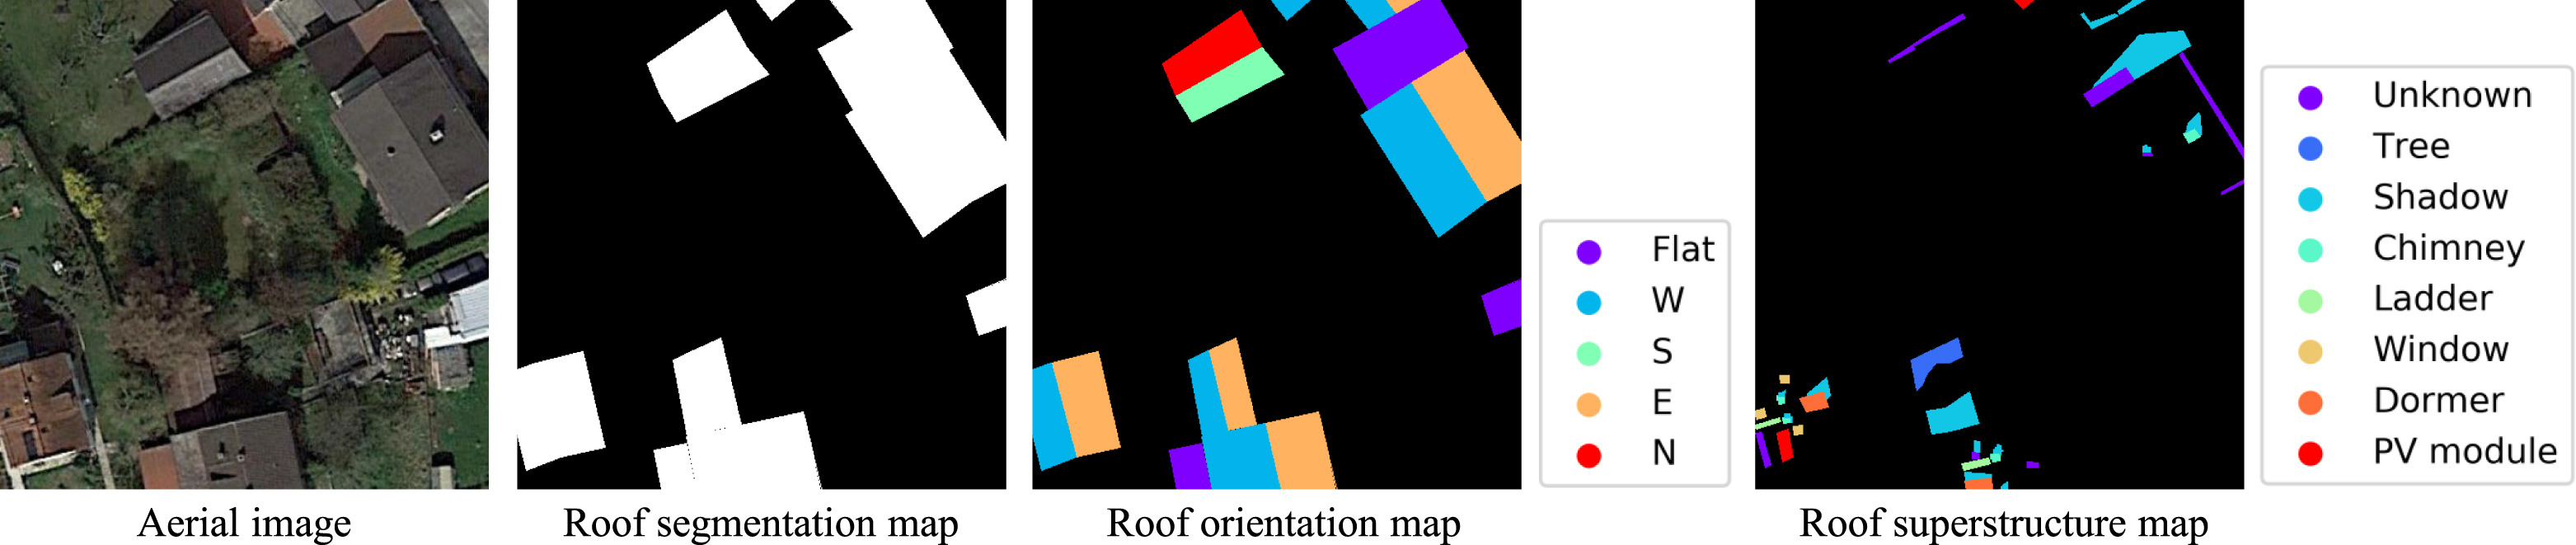
\includegraphics[width=1\linewidth]{02-main//figures/ch2/rid_dataset_sample.png}
    \caption{Exemple d'image du dataset RID \cite{li_deep_2024}}
    \label{fig:rid_dataset_sample}
\end{figure}

\subsubsection{Méthodologie}
\par{SolarNet+ utilise une approche en deux étapes :}
\begin{enumerate}
    \item Un réseau de neurones multi fonctions (partie 1 de la Figure \ref{fig:solar_net_plus_methodo}) va réaliser les opérations suivantes sur chaque image:
    \begin{itemize}
        \item Segmenter l'image pour avoir le masque de la toiture ainsi que son orientation géographique ("Roof orientation map" de la Figure \ref{fig:solar_net_plus_methodo}).
        \item Segmenter les éléments de toiture pour identifier tous les obstacles qui s'y trouvent ("Roof superstructure map" de la Figure \ref{fig:solar_net_plus_methodo}).
        \item Extraire les surfaces exploitables de toiture par superposition des masques. Cette étape consiste à soustraire les zones occupées par les obstacles ("Roof superstructure map") des segments de toiture identifiés ("Roof orientation map"), permettant ainsi d'isoler les surfaces disponibles.
    \end{itemize}
    \item Estimer le potentiel solaire pour chaque surface identifiée (partie 2 de la Figure \ref{fig:solar_net_plus_methodo}) qui comprend :
    \begin{itemize}
        \item Hypothèses de base pour le calcul :
        \begin{itemize}
            \item Panneau PV 1.7 \si{\unit{\square\meter}} avec 400 Wc
            \item Pente toiture 30° pour toutes les orientations sauf toiture plate 0°
            \item Pans de toiture de moins de 5 \si{\unit{\square\meter}} ne sont pas considérés comme surface disponible
        \end{itemize}
        \item Calcul du nombre maximum de panneaux installables sur chaque segment de toiture disponible, en tenant compte des contraintes géométriques. La Figure \ref{fig:solar_net_plus_placement_pv}) présente deux exemples, avec et sans obstacles sur la toiture. Le placement des panneaux commence du côté gauche en bas et va éviter les obstacles présents.
        \item Acquisition des données d'irradiation solaire spécifiques à chaque orientation via l'API PVGIS
        \item Estimation de l'énergie annuelle générée pour chaque pans de toiture en multipliant le nombre de panneaux installables par la production unitaire correspondant à l'orientation
        \item Additionner les potentiels de tous les pans de toiture pour obtenir le potentiel solaire total du bâtiment
    \end{itemize}
\end{enumerate}

\begin{figure}[H]
    \makebox[\textwidth][c]{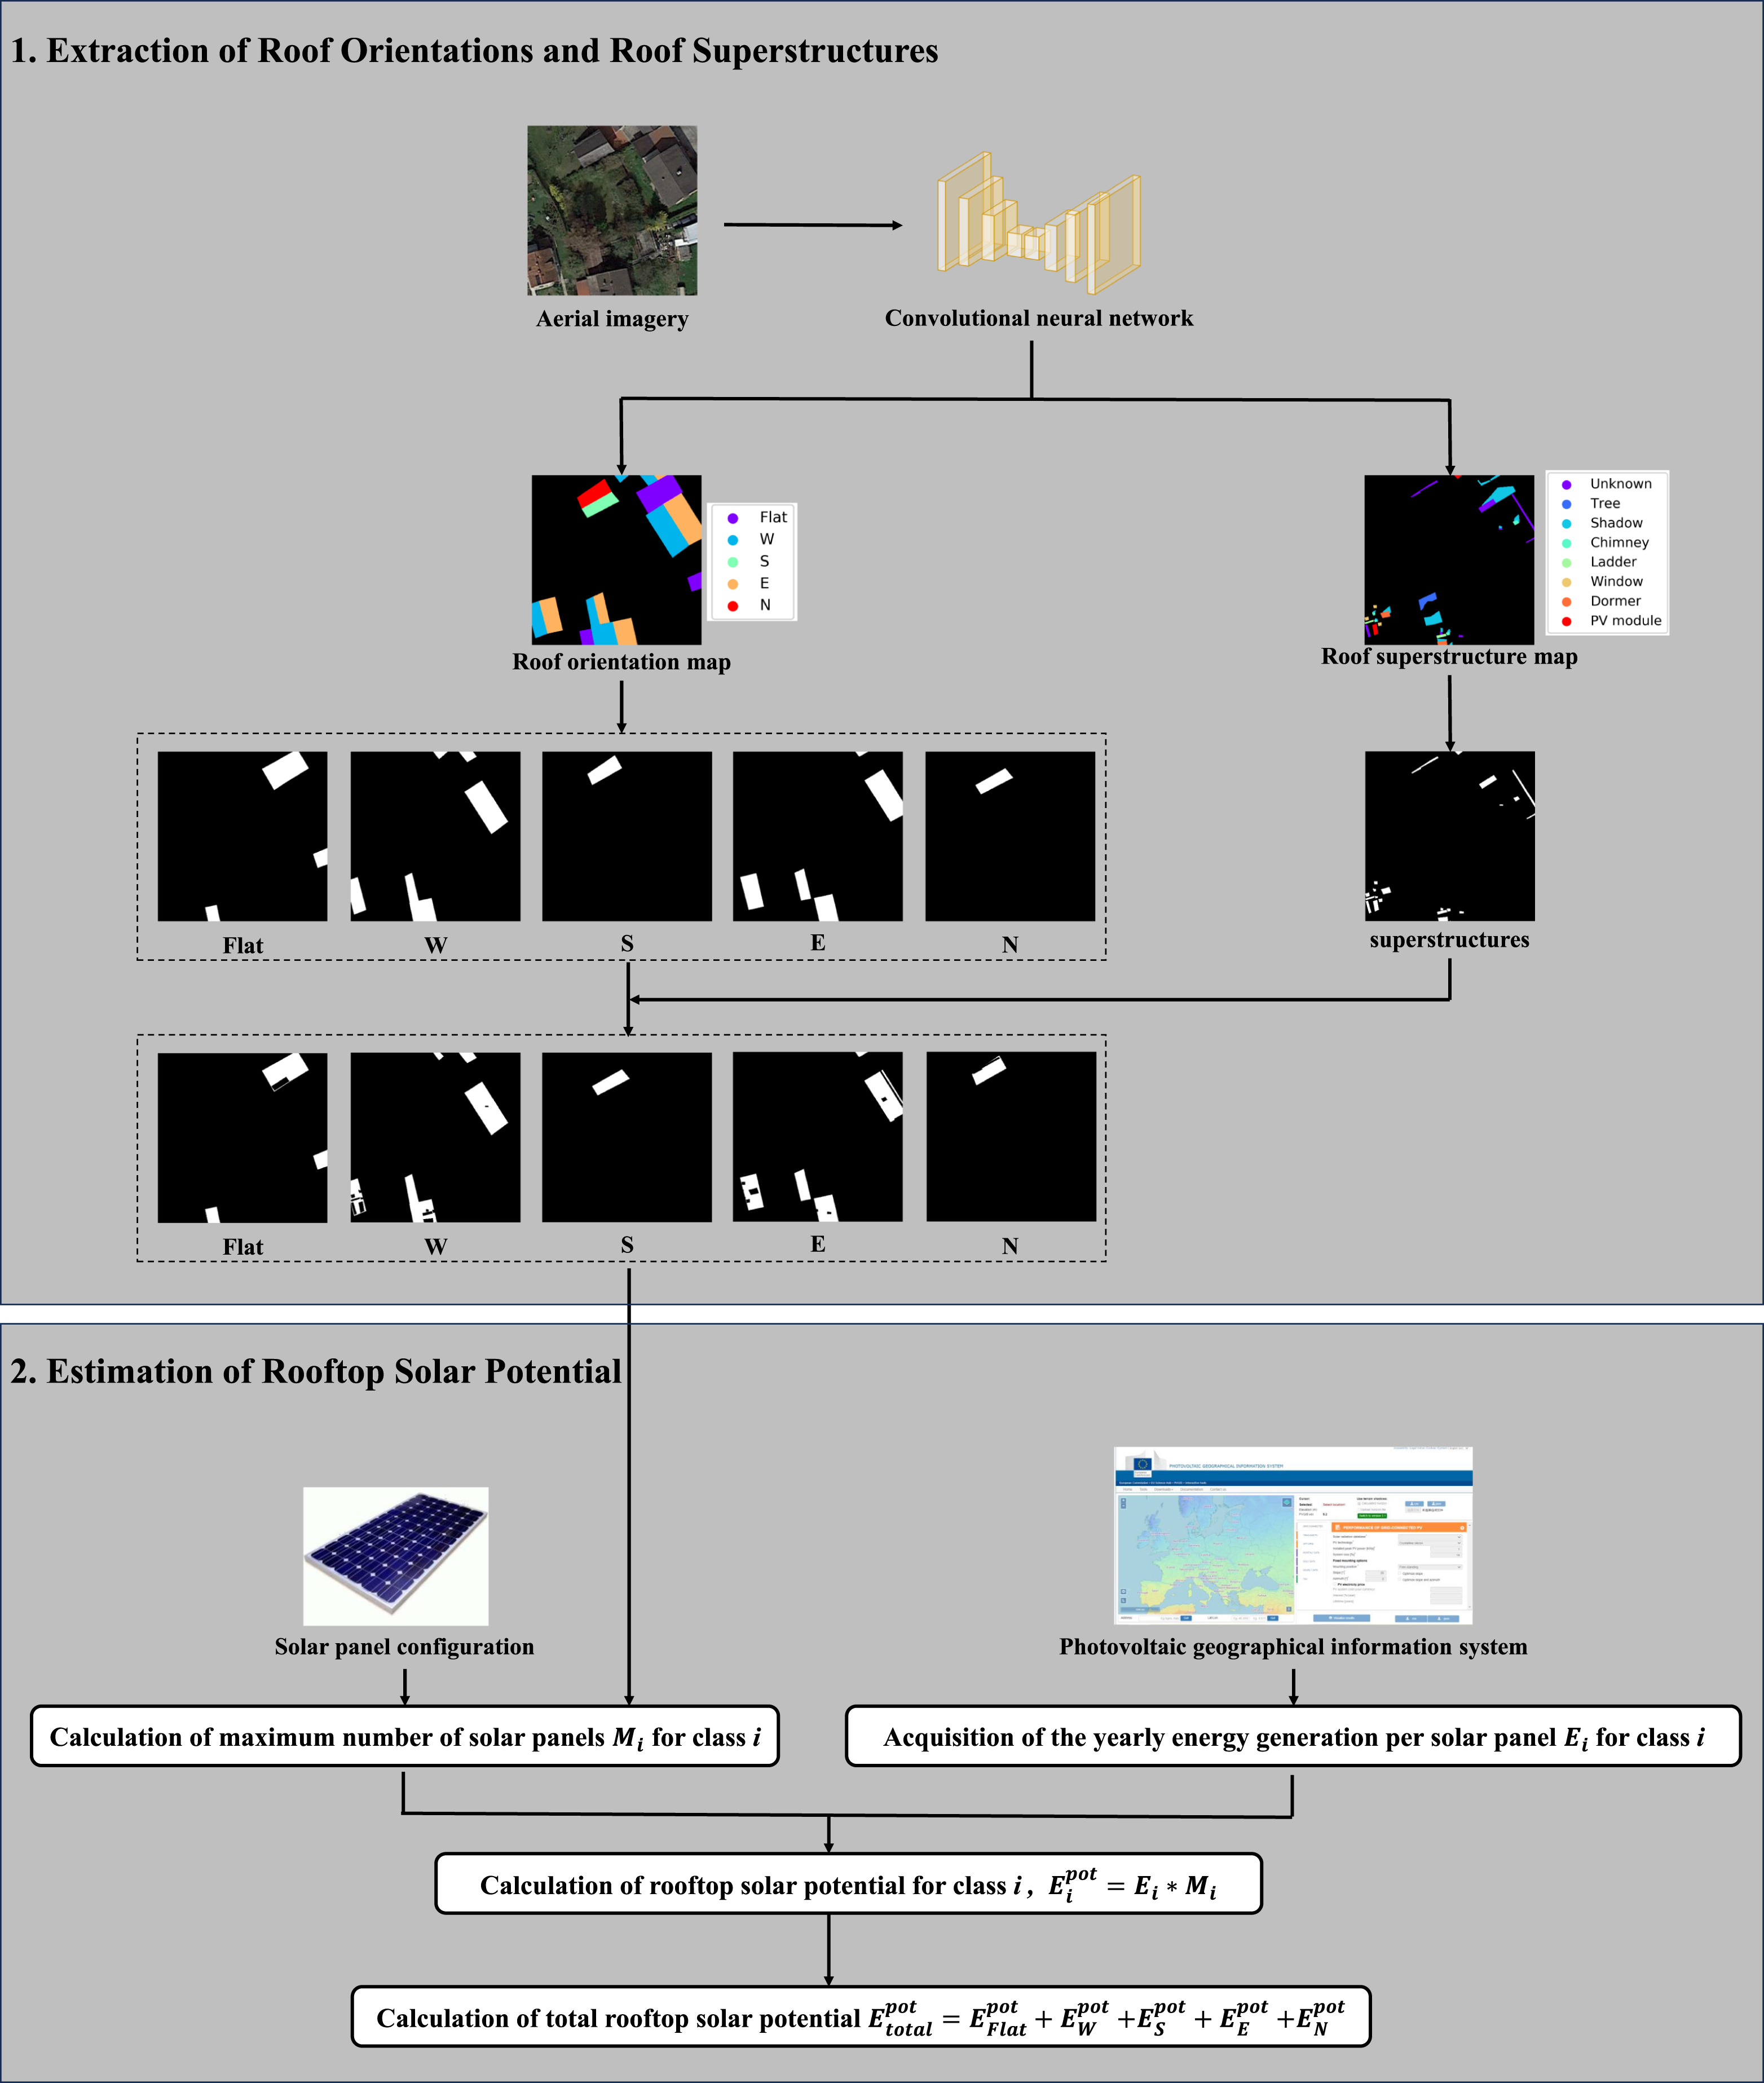
\includegraphics[width=1.1\textwidth]{02-main//figures/ch2/solar_net_plus_methodo.png}}
    \caption{Méthodologie SolarNet+ \cite{li_deep_2024}}
    \label{fig:solar_net_plus_methodo}
\end{figure}

\begin{figure}[H]
    \centering
    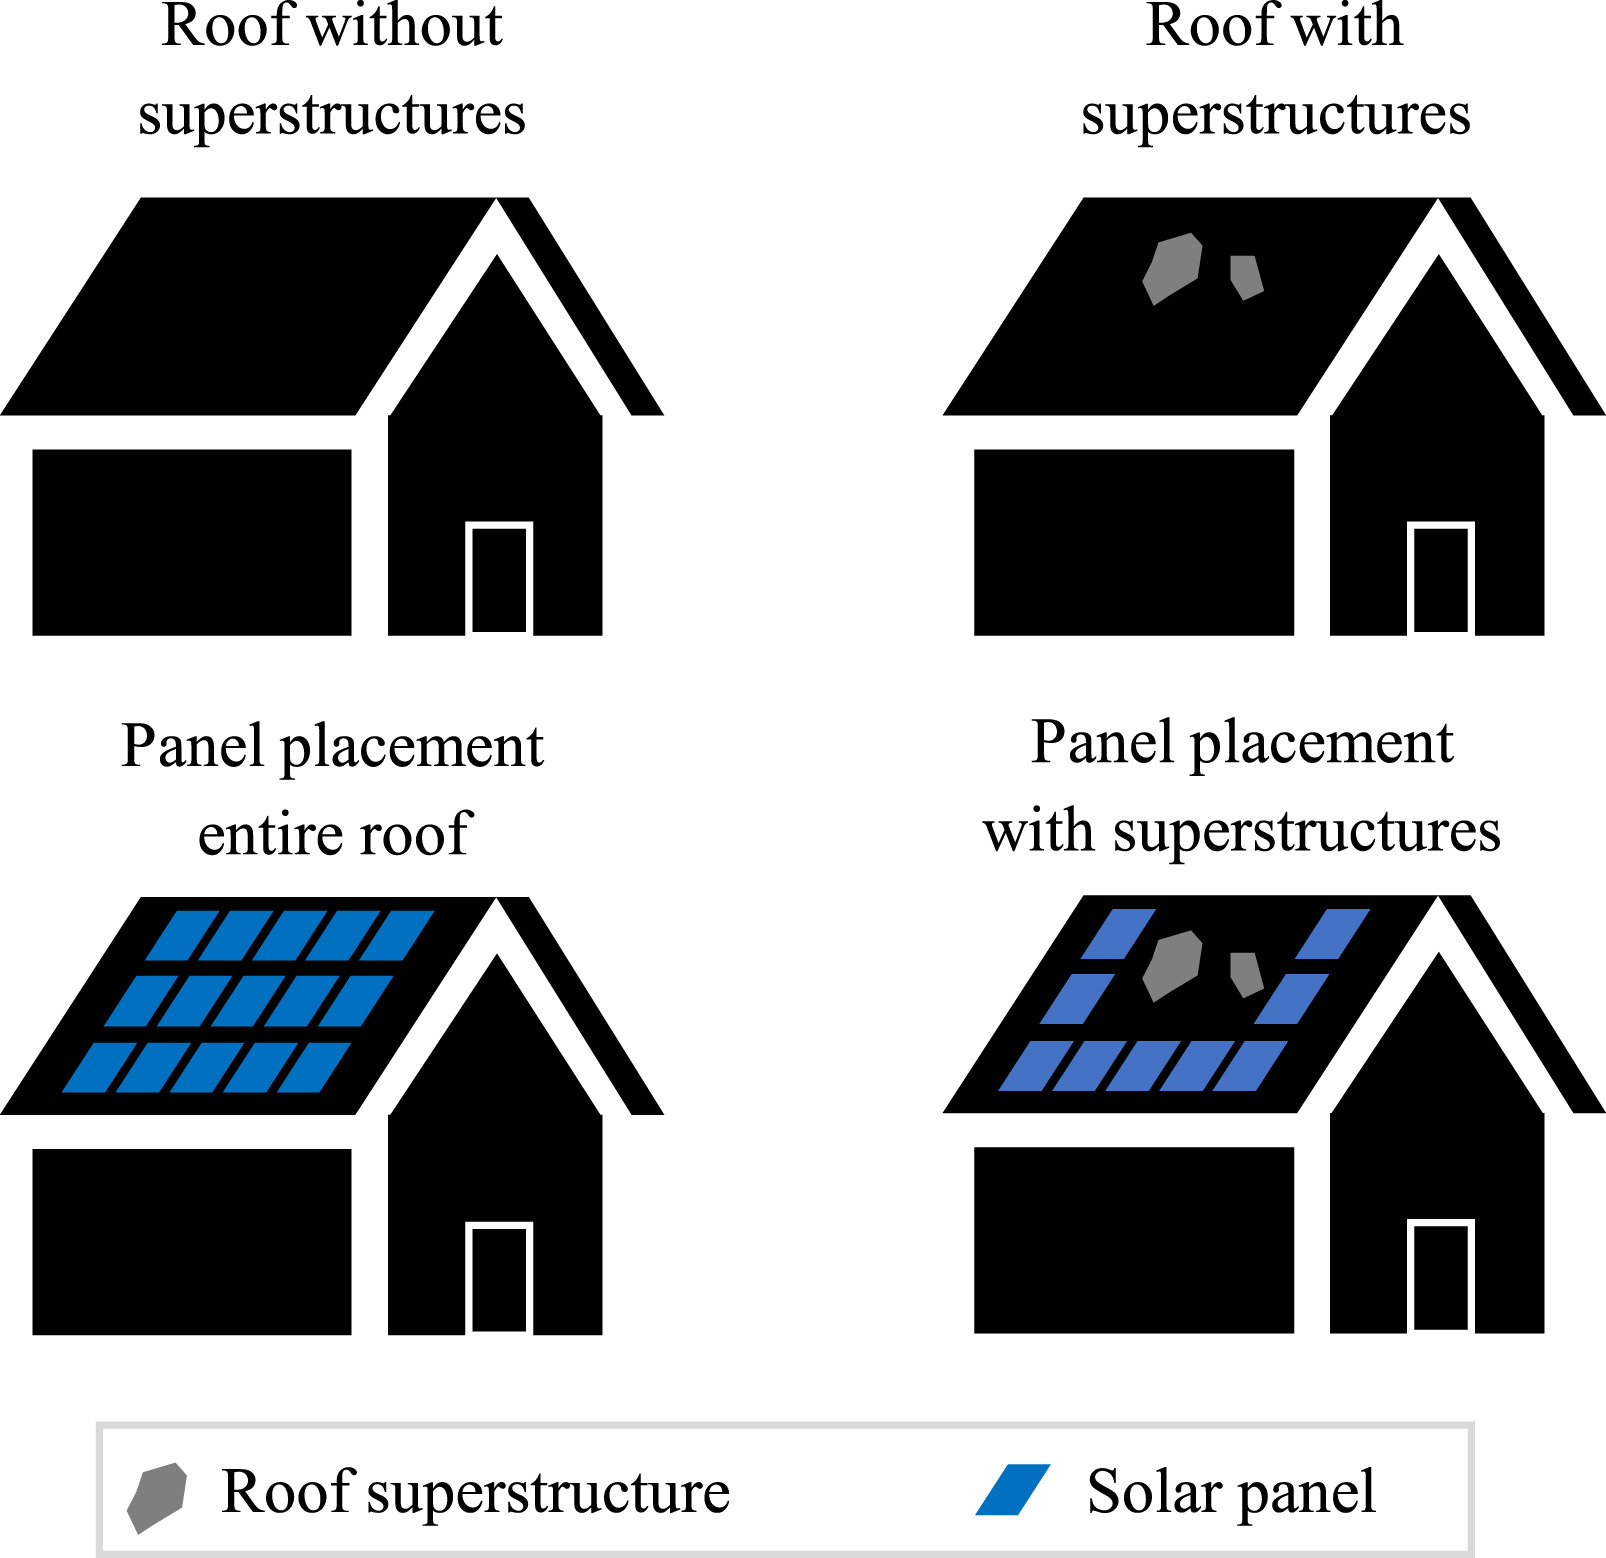
\includegraphics[width=0.5\linewidth]{02-main//figures/ch2/solar_net_plus_placement_pv.png}
    \caption{Placement des panneaux solaire \cite{li_deep_2024}}
    \label{fig:solar_net_plus_placement_pv}
\end{figure}

\par{La Figure \ref{fig:solar_net_plus_exemple_methodo} permet d'avoir un aperçu des différentes phases du calcul de potentiel solaire. En allant de gauche à droite dans la lecture de la Figure \ref{fig:solar_net_plus_exemple_methodo}, les deux premières images indiquent l'irradiation solaire avec et sans les obstacles. En bas à gauche de ces deux images, on peut observer une toiture avec plusieurs obstacles détectés (trous), sans les obstacles son irradiation solaire est bonne, mais avec les obstacles son irradiation solaire totale est réduite. La troisième image représente le placement des panneaux solaires. Finalement la quatrième image, représente le potentiel solaire total par pan de toiture selon le nombre de panneaux solaire placés dans la troisième image et l'irradiation solaire de la deuxième image.}

\begin{figure}[H]
    \makebox[\textwidth][c]{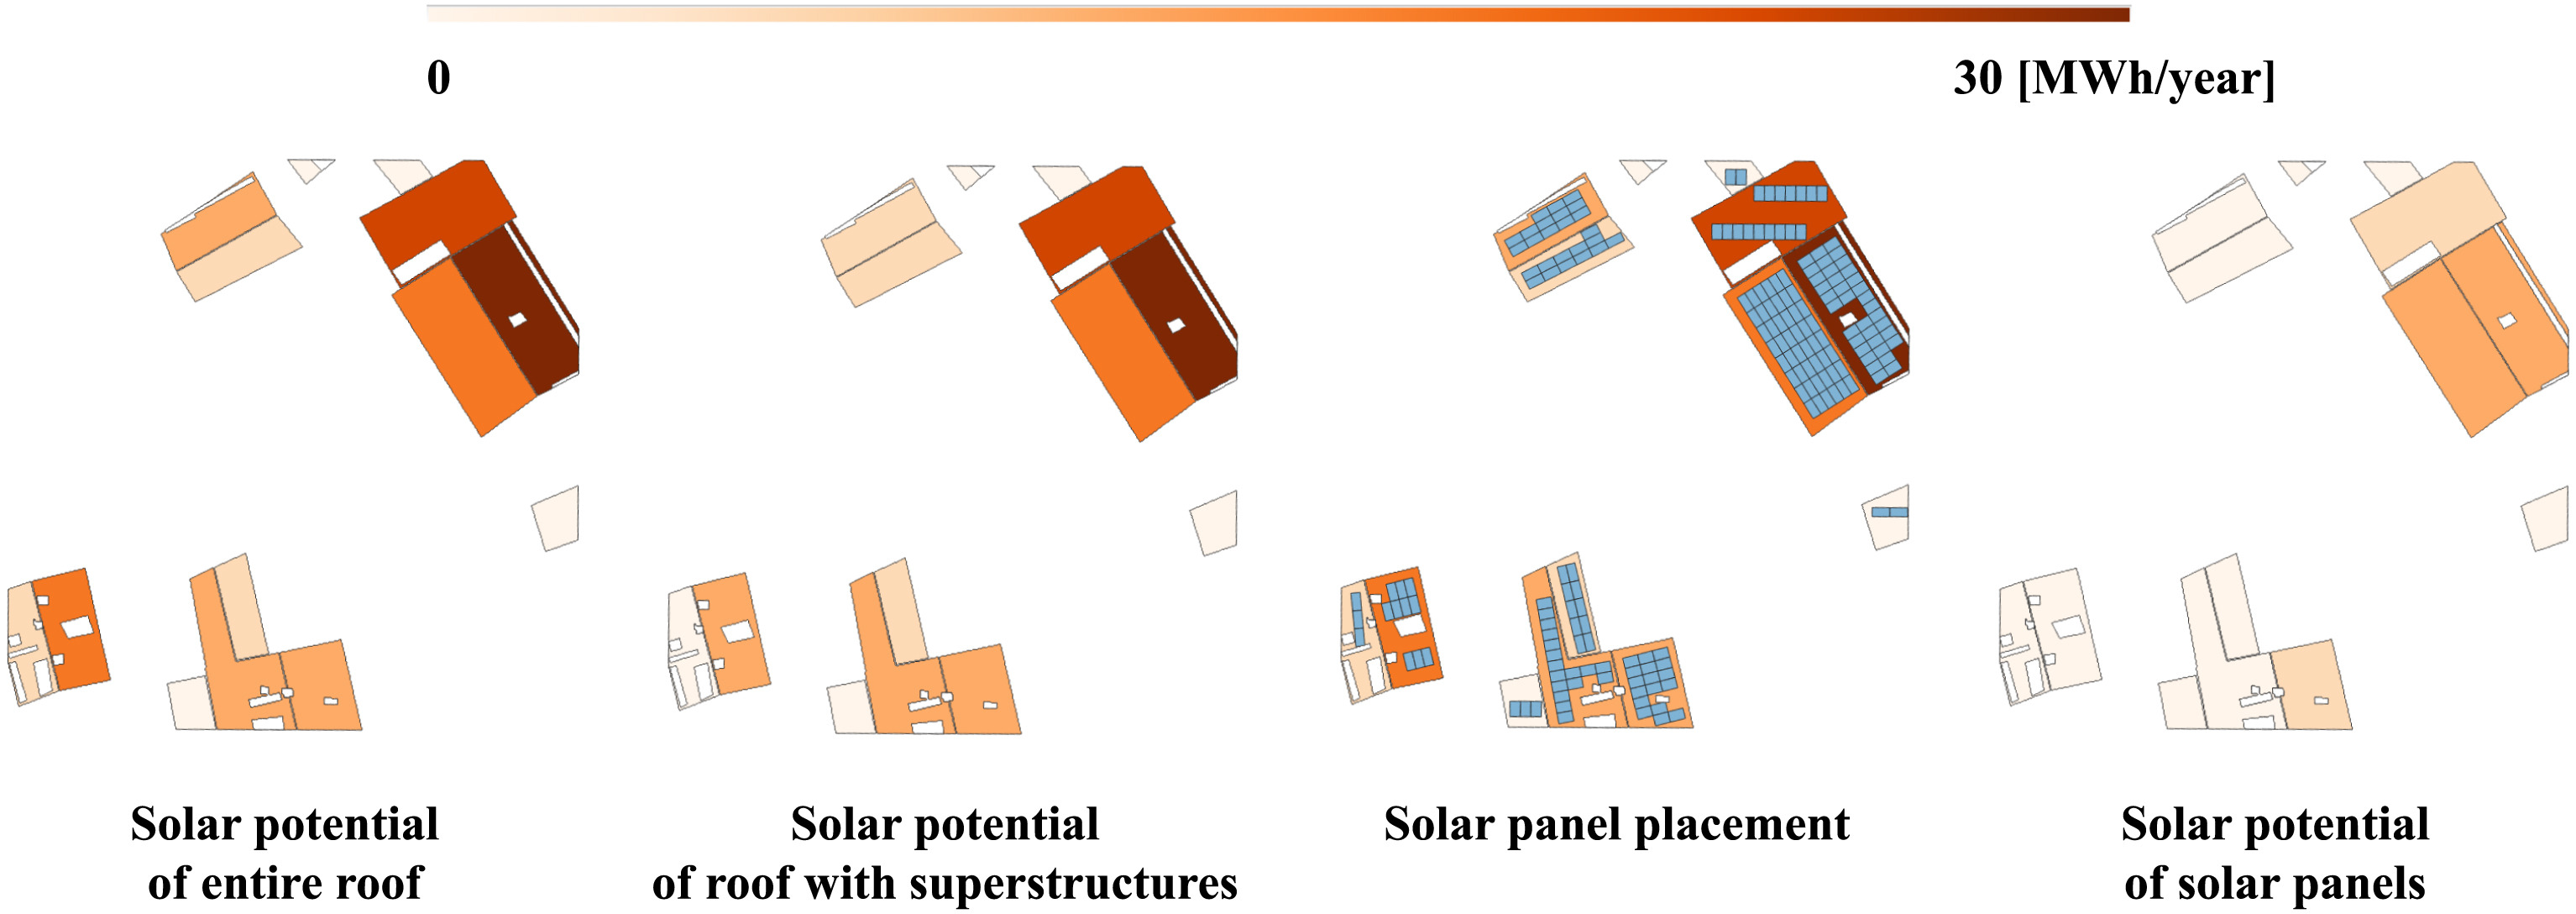
\includegraphics[width=1.15\textwidth]{02-main//figures/ch2/solar_net_plus_exemple_methodo.png}}
    \caption{Exemple d'application de la méthodologie \cite{li_deep_2024}}
    \label{fig:solar_net_plus_exemple_methodo}
\end{figure}

\subsubsection{Résultats principaux}
\begin{itemize}
    \item SolarNet+ surpasse les réseaux concurrents en termes de précision pour la prédiction de l'orientation des toits et des superstructures avec les meilleures performances en mIoU et OA.
    \item L'étude montre que négliger les superstructures conduit à une surestimation de 42\% du nombre de panneaux solaires installables.
    \item La précision d'estimation du potentiel solaire atteint un \%RMSE de 19,92\% par rapport la vérité terrain (détail des résultats dans la Table \ref{tab:solar_net_plus_comparaison_quant}).
\end{itemize}

\begin{table}[H]
    \centering
    \small
    \begin{tabular}{lrrrr}
        \toprule
        \textbf{Méthode} & \textbf{Nombre de panneaux} & \textbf{Potentiel solaire} & \textbf{RMSE} & \textbf{\%RMSE} \\
        & \textbf{installables} & \textbf{(MWh/an)} & \textbf{(MWh/an)} & \\
        \midrule
        U-Net & 25 855 & 8484,28 & 12,77 & 21,49 \\
        FC-DenseNet & 29 316 & 9544,90 & 20,85 & 35,10 \\
        Efficient-UNet & 23 842 & 7754,68 & 16,85 & 28,37 \\
        DeepLab V3+  & 28 152 & 9153,37 & 25,14 & 42,32 \\
        Srivastava et al. & 24 987 & 8125,64 & 12,63 & 21,27 \\
        Bischke et al. & 25 749 & 8446,82 & 14,34 & 24,13 \\
        Mou \& Zhu & 24 945 & 8075,86 & 14,22 & 23,93 \\
        \textbf{SolarNet+} & \textbf{24 541} & \textbf{7967,34} & \textbf{11,83} & \textbf{19,92} \\
        \midrule
        Ground truth & 24 279 & 7959,76 & - & - \\
        \bottomrule
    \end{tabular}
    \caption{Résultats quantitatifs du potentiel solaire sur le dataset RID \cite{li_deep_2024}}
    \label{tab:solar_net_plus_comparaison_quant}
\end{table}


\subsubsection{Discussion et limites}
\begin{itemize}
    \item La démarche utilisée par cet article est assez unique, c'est le seul article qui va aussi loin dans la segmentation des toitures et l'identification des obstacles. Le dataset RID est disponible librement et il a été réalisé par les auteurs de cet article.
    \item Les auteurs ont testé le modèle avec des images satellite de Bruxelles (le dataset RID inclus seulement Wartenberg à Munich), mais les performances diminuent en raison des différences architecturales et des superstructures non rencontrées dans les données d'entraînement (balcons, éléments technique de ventilation/climatisation, etc.).
    \item Le modèle ne prend pas en compte les ombrages, ce qui peut réduire significativement l'irradiation solaire reçue par un pan de toiture.
    \item Les auteurs suggèrent d'intégrer des données 3D et cela semble une bonne initiative pour des futures évolutions du framework. Avec des données \gls{lidar}, ils pourraient nettement améliorer la phase de post-processing des pans de toiture en intégrant les ombrages et une meilleure estimation des pentes des toitures.
\end{itemize}

% -----------------------------------------------------------------------------
\subsection{Quantification of the suitable rooftop area for solar panel installation from overhead imagery using Convolutional Neural Networks}
\label{subsec:castello_quantification_2021}

\subsubsection{Contexte et objectifs}
\par{Cet article \cite{castello_quantification_2021} présente une approche innovante pour quantifier les surfaces disponibles sur les toitures pour l'installation de panneaux solaires photovoltaïques. Face au défi de l'évaluation précise du potentiel solaire à grande échelle, \citeauthor{castello_quantification_2021} proposent une méthode combinant le deep learning, la vision par ordinateur et des données de bâtiments 3D.}

\subsubsection{Méthodologie}
\par{L'approche utilise un réseau de neurones convolutif (CNN) basé sur l'architecture U-Net, adapté pour la segmentation sémantique d'images aériennes à haute résolution. Le modèle a été entraîné sur 524 images (orthophotos de swisstopo 2015) de taille 250x250 pixels de Genève, avec une résolution spatiale de 0,25 m/pixel. Les données d'entraînement ont été annotées manuellement (classe unique "libre") pour identifier les zones disponibles sur les toits. Ces données ne sont pas disponibles.}

\par{La méthodologie comporte trois étapes principales :}
\begin{enumerate}
    \item Traitement des images aériennes par le CNN pour identifier les surfaces disponibles
    \item Post-traitement géospatial combinant les résultats avec la couche \acrshort{sitg} des toitures
    \item Les toitures de moins de 10 \si{\unit{\square\meter}} ne sont pas considérées comme toiture disponible
\end{enumerate}

\par{Les auteurs ont également implémenté diverses techniques d'augmentation de données et optimisé les hyperparamètres du modèle pour améliorer ses performances.}

\subsubsection{Résultats principaux}
Le CNN développé atteint :
\begin{itemize}
    \item Une précision de 93\% dans l'identification des surfaces disponibles
    \item Un score d'Intersection over Union (IoU) de 64\%
    \item Une sous-estimation moyenne de 8\% des surfaces disponibles par rapport aux annotations manuelles
\end{itemize}
\par{Le Tableau \ref{tab:castello_quantification_resultats} ci-dessous détaille les résultats obtenus:}
\begin{table}[H]
    \centering
    \begin{tabular}{|l|c|c|c|c|c|}
    \hline
     & IoU & Accuracy & Recall & Precision & F1-score \\
    \hline
    Training & 0.8823 & 0.9794 & 0.9299 & 0.9437 & 0.9367 \\
    Validation & 0.7211 & 0.9464 & 0.8360 & 0.8508 & 0.8433 \\
    Test & 0.6420 & 0.9307 & 0.7522 & 0.7874 & 0.7693 \\
    \hline
    \end{tabular}
    \caption{Performances du modèle U-Net développé}
\label{tab:castello_quantification_resultats}
\end{table}

\par{Le modèle réussit à détecter automatiquement les obstacles présents sur les toits, y compris les panneaux solaires existants, fenêtres, cheminées, équipements techniques et zones ombragées. L'étude révèle que la fraction médiane de la surface disponible varie selon la taille des toits :}
\begin{itemize}
    \item 61\% pour les grands toits (>500 m²)
    \item 77\% pour les toits moyens (100-500 m²)
    \item 80\% pour les petits toits (10-100 m²)
\end{itemize}

\par{La Figure \ref{fig:castello_quantification_image_resultat} permet de voir deux exemples de résultat.}
\begin{figure}[H]
    \centering
    \begin{subfigure}{0.44\textwidth}
        \centering
        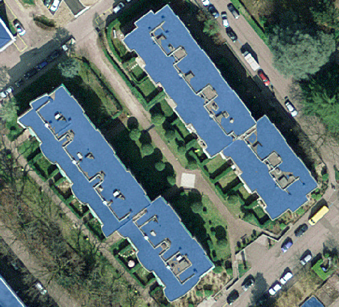
\includegraphics[width=\textwidth]{02-main//figures/ch2/castello_quantification_image_resultat1.png}
        \caption{Grandes toitures plates}
        \label{fig:castello_quantification_image_resultat1}
    \end{subfigure}
    \hfill
    \begin{subfigure}{0.43\textwidth}
        \centering
        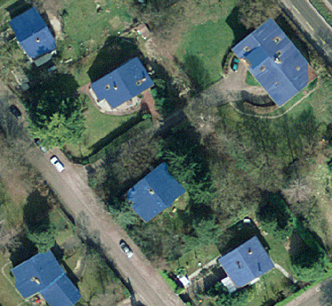
\includegraphics[width=\textwidth]{02-main//figures/ch2/castello_quantification_image_resultat2.png}
        \caption{Toitures en pente}
        \label{fig:castello_quantification_image_resultat2}
    \end{subfigure}
    \caption{Images d'exemple \cite{castello_quantification_2021} du résultat après inférence. Les zones bleus sont les espaces disponibles.}
    \label{fig:castello_quantification_image_resultat}
\end{figure}

\par{La comparaison avec d'autres méthodes d'estimation montre que les approches existantes tendent à surestimer la surface disponible sur les grands toits et à sous-estimer celle des petits toits.}

\subsubsection{Discussion et limites}
\par{L'article présente une approche prometteuse pour quantifier les surfaces de toiture disponibles pour l'installation solaire. Le modèle U-Net atteint un IoU de 64\% et une précision de 93\% sur les données de test, avec la capacité notable d'exclure automatiquement les zones ombragées des toits.}
\par{La comparaison avec les méthodes existantes révèle des différences selon la taille des bâtiments. Pour les grandes toitures, le modèle CNN estime une fraction médiane de surface disponible de 39\% contre 66\% pour l'approche de référence, suggérant une surestimation des méthodes à grande échelle. Pour les petites toitures, la tendance s'inverse avec 47\% contre 32\%.}
\par{Le modèle sous-estime en moyenne de 8\% la surface réellement disponible par rapport à la vérité terrain. Cette sous-estimation est principalement observée sur les petites toitures (< 100 m²). Les limites identifiées incluent la difficulté à détecter les lucarnes, construites dans le même matériau que le toit, et les zones de "toits verts" avec végétation.}
\par{L'étude se limite au centre de Genève avec 524 images principalement résidentielles. Les auteurs mentionnent 12 heures de labellisation manuelle sans préciser la répartition du travail. Pour une extension nationale, ils proposent l'ajout d'un canal infrarouge et l'utilisation d'images plus récentes à haute résolution.}

% -----------------------------------------------------------------------------

\subsection{YOLOv12: Attention-Centric Real-Time Object Detectors}

\subsubsection{Contexte et objectifs}
La détection d'objets en temps réel repose traditionnellement sur les réseaux de neurones convolutionnels (CNN) dans la famille YOLO. Cependant, les mécanismes d'attention, popularisés par les ``Vision Transformers'', offrent de meilleures capacités de modélisation grâce à leur capacité à capturer les dépendances globales dans l'image. Le problème fondamental est que l'attention a un coût computationnel élevé : sa complexité croît quadratiquement avec la taille de l'image ($O(n^2)$), là où les convolutions croissent linéairement ($O(n)$). 

YOLOv12 relève ce défi en proposant le premier framework YOLO centré sur l'attention qui atteint la vitesse des modèles CNN traditionnels tout en conservant les avantages de performance de l'attention. L'objectif est de démontrer qu'il est possible de casser la domination des CNN dans YOLO.

\subsubsection{Données}
L'évaluation utilise le dataset de référence MS COCO 2017 pour la détection d'objets. Cinq variantes de modèles sont développées (YOLOv12-N/S/M/L/X) correspondant à différentes tailles et complexités. L'entraînement suit le protocole standard : 600 époques avec l'optimiseur SGD, augmentations de données classiques (Mosaic, Mixup, copy-paste). Les performances sont mesurées sur GPU T4 avec TensorRT FP16 pour assurer la reproductibilité.

\subsubsection{Méthodologie}
YOLOv12 introduit trois innovations clés pour rendre l'attention efficace :
\begin{itemize}
    \item Réduction de la complexité (Area Attention)
    \item Stabilisation de l'entraînement (R-ELAN)
    \item Améliorations architecturales
\end{itemize}

\paragraph{Area Attention (A2)}
Plutôt que de calculer l'attention sur toute l'image (coûteux), la carte de caractéristiques est divisée en zones rectangulaires (par défaut 4 segments). L'attention n'est calculée qu'à l'intérieur de chaque zone, réduisant la complexité de moitié tout en préservant un champ réceptif suffisant. C'est l'équivalent de regarder plusieurs « fenêtres » de l'image simultanément plutôt que l'image entière.

Le mécanisme d'attention (Figure \ref{fig:ch2_yolo_mecanismes_attention}) local est simplifié par rapport aux autres alternatives (Figures \ref{fig:ch2_yolo_01_attention_area_criss_cross}, \ref{fig:ch2_yolo_02_attention_area_window} et \ref{fig:ch2_yolo_03_attention_area_criss_axial}). Celui-ci divise la carte de caractéristiques en $l$ segments (par défaut 4) verticalement (Figure \ref{fig:ch2_yolo_05_attention_area_yolo2}) ou horizontalement (Figure \ref{fig:ch2_yolo_04_attention_area_yolo1}), réduisant la complexité tout en maintenant un large champ réceptif.

\begin{figure}[H]
    \centering
    \begin{subfigure}[b]{0.30\textwidth}
        \centering
        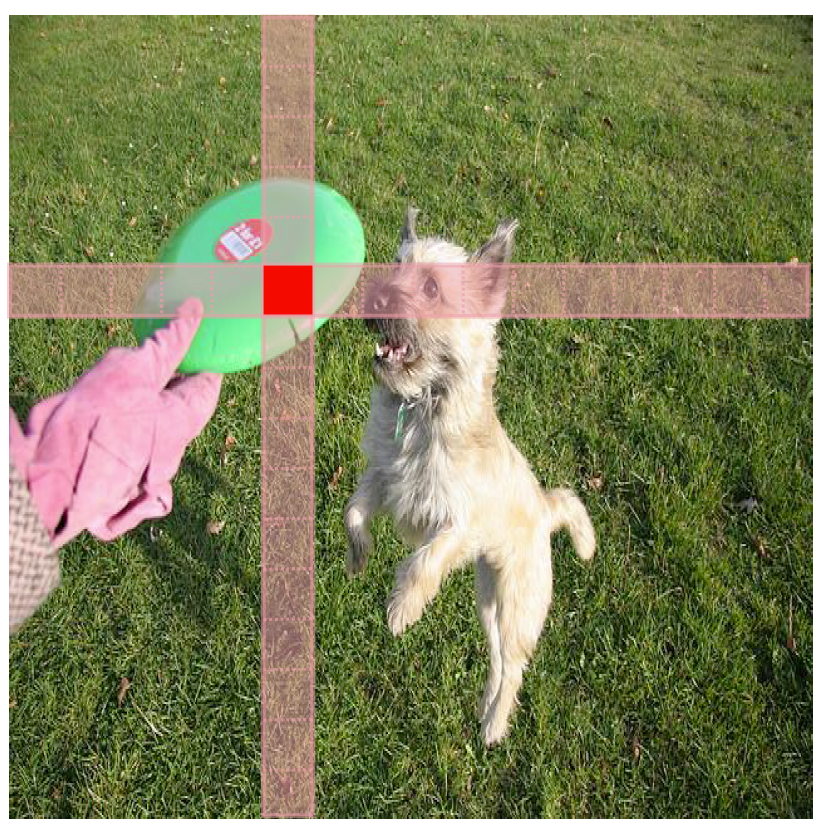
\includegraphics[width=\textwidth]{02-main/figures/ch2/ch2_yolo_01_attention_area_criss_cross.png}
        \caption{Mécanisme d'attention type ``criss cross''}
        \label{fig:ch2_yolo_01_attention_area_criss_cross}
    \end{subfigure}
    \hfill
    \begin{subfigure}[b]{0.30\textwidth}
        \centering
        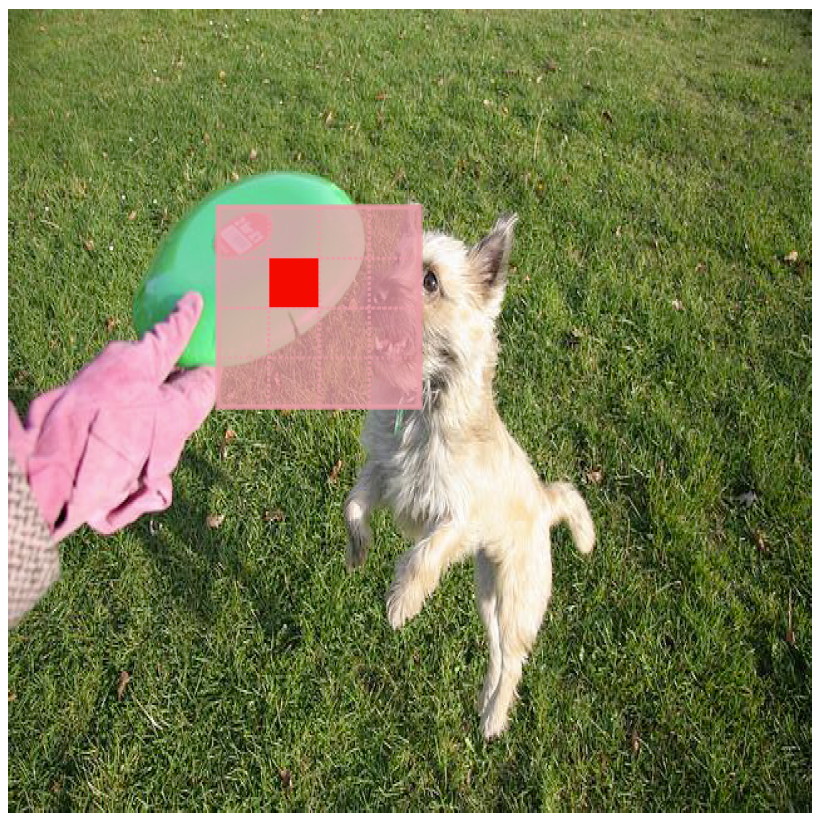
\includegraphics[width=\textwidth]{02-main/figures/ch2/ch2_yolo_02_attention_area_window.png}
        \caption{Mécanisme d'attention type ``fenêtre''}
        \label{fig:ch2_yolo_02_attention_area_window}
    \end{subfigure}
    \hfill
    \begin{subfigure}[b]{0.30\textwidth}
        \centering
        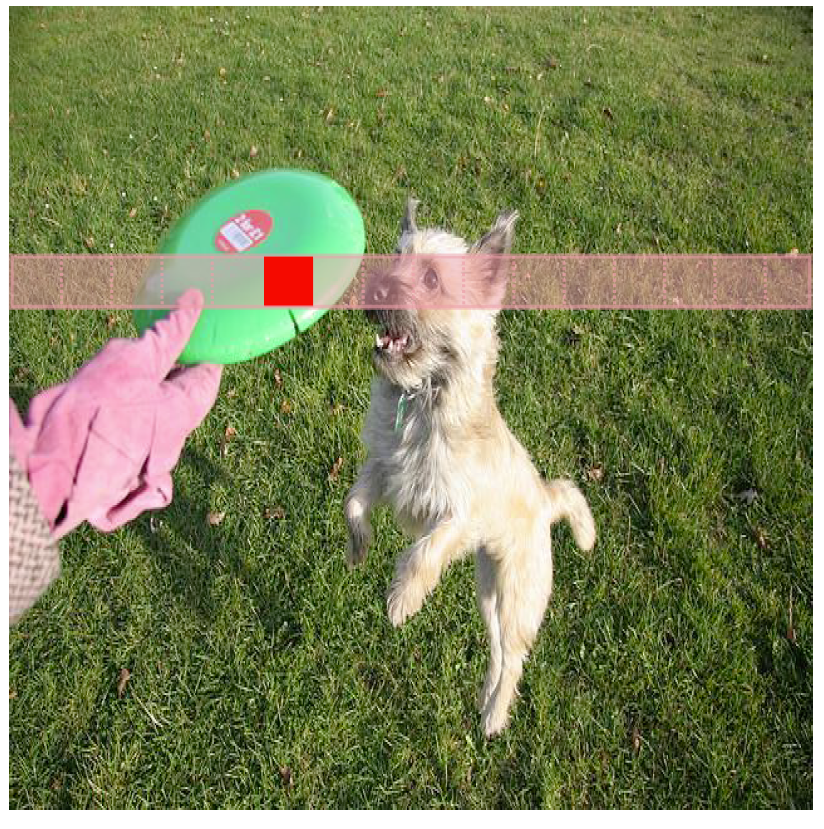
\includegraphics[width=\textwidth]{02-main/figures/ch2/ch2_yolo_03_attention_area_criss_axial.png}
        \caption{Mécanisme d'attention type ``axial''}
        \label{fig:ch2_yolo_03_attention_area_criss_axial}
    \end{subfigure}

    \vspace{0.35cm}
    \begin{subfigure}[b]{0.30\textwidth}
        \centering
        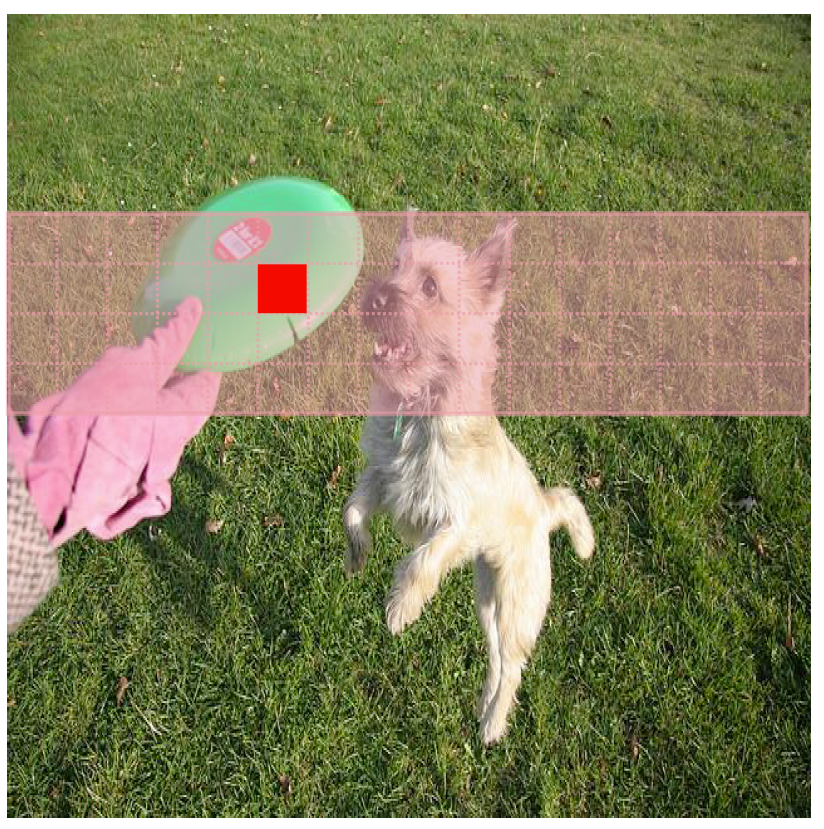
\includegraphics[width=\textwidth]{02-main/figures/ch2/ch2_yolo_04_attention_area_yolo1.png}
        \caption{Mécanisme d'attention horizontal proposé dans YOLOv12}
        \label{fig:ch2_yolo_04_attention_area_yolo1}
    \end{subfigure}
    \hspace{0.04\textwidth}
    \begin{subfigure}[b]{0.30\textwidth}
        \centering
        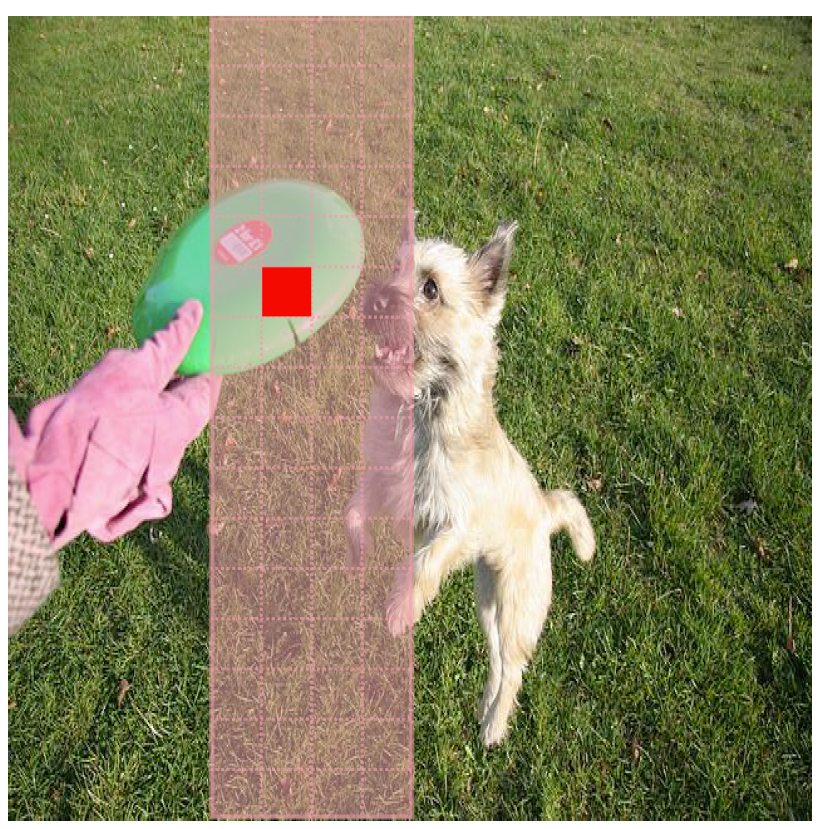
\includegraphics[width=\textwidth]{02-main/figures/ch2/ch2_yolo_05_attention_area_yolo2.png}
        \caption{Mécanisme d'attention vertical proposé dans YOLOv12}
        \label{fig:ch2_yolo_05_attention_area_yolo2}
    \end{subfigure}    
    \caption{Mécanismes d'attention \cite{tian_yolov12_2025}}
    \label{fig:ch2_yolo_mecanismes_attention}
\end{figure}

\paragraph{R-ELAN}
Les mécanismes d'attention rendent l'entraînement instable, particulièrement pour les gros modèles. La Figure \ref{fig:ch2_yolo_architecture_simplifiee} illustre l'évolution progressive des architectures de blocs dans la famille YOLO, depuis les premières approches jusqu'à la proposition YOLOv12.

CSPNet (Figure \ref{fig:ch2_yolo_06_architecture_csp}), utilisé dans YOLOv4/YOLOv5, est l'architecture fondatrice qui divise le flux de données en deux branches parallèles, permettant un meilleur gradient flow et réduisant les calculs redondants. Une branche traverse directement, l'autre passe par plusieurs blocs convolutionnels avant concaténation.

ELAN (Figure \ref{fig:ch2_yolo_07_architecture_elan}), utilisé dans YOLOv7, correspond aux Efficient Layer Aggregation Networks qui améliorent l'agrégation de caractéristiques en connectant explicitement différentes couches. Cette architecture permet une meilleure réutilisation des caractéristiques, mais souffre de problèmes de stabilité d'optimisation, particulièrement visibles dans les gros modèles.

$C_3K_2$ (Figure \ref{fig:ch2_yolo_08_architecture_c3k2}), utilisé dans YOLOv11, est l'évolution de GELAN (Generalized ELAN) qui simplifie l'architecture tout en conservant l'efficacité. $C_3K_2$ représente un cas particulier optimisé de GELAN, adopté pour réduire la latence dans YOLOv11.

R-ELAN (Figure \ref{fig:ch2_yolo_09_architecture_relan}) est l'architecture de bloc proposée dans YOLOv12. La contribution majeure des Residual Efficient Layer Aggregation Networks est l'ajout d'une connexion résiduelle avec facteur d'échelle (scaling) depuis l'entrée vers la sortie, inspirée des techniques de Vision Transformers. Cette modification résout les problèmes de convergence observés avec les mécanismes d'attention, particulièrement critiques pour les modèles YOLOv12-L et YOLOv12-X qui ne convergent pas sans cette stabilisation.


\begin{figure}[H]
    \centering
    \begin{subfigure}[b]{0.30\textwidth}
        \centering
        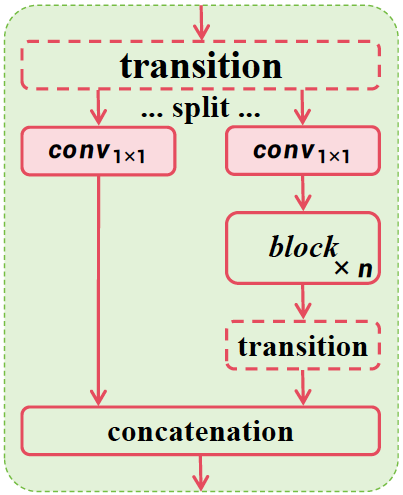
\includegraphics[width=\textwidth]{02-main/figures/ch2/ch2_yolo_06_architecture_csp.png}
        \caption{``CSPNet'' (YOLOv4/v5)}
        \label{fig:ch2_yolo_06_architecture_csp}
    \end{subfigure}
    \hfill
    \begin{subfigure}[b]{0.30\textwidth}
        \centering
        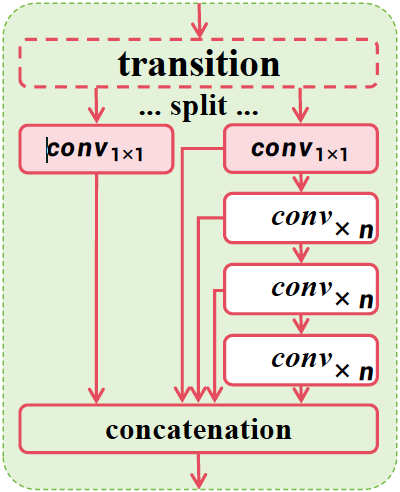
\includegraphics[width=\textwidth]{02-main/figures/ch2/ch2_yolo_07_architecture_elan.png}
        \caption{``ELAN'' (YOLOv7)}
        \label{fig:ch2_yolo_07_architecture_elan}
    \end{subfigure}
    \vspace{0.35cm}
    \begin{subfigure}[b]{0.45\textwidth}
        \centering
        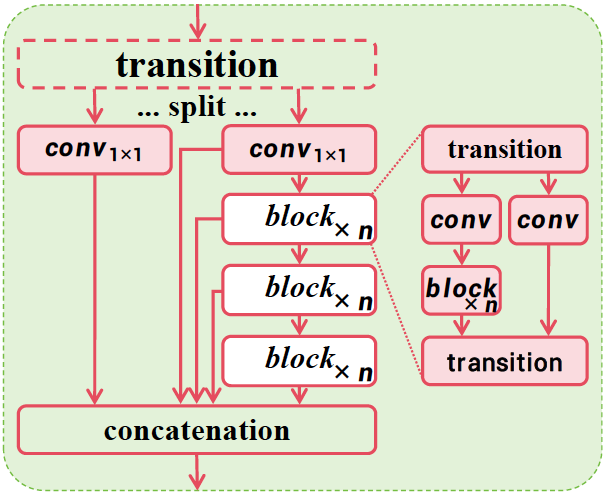
\includegraphics[width=\textwidth]{02-main/figures/ch2/ch2_yolo_08_architecture_c3k2.png}
        \caption{``$C_3K_2$'' (YOLOv11)}
        \label{fig:ch2_yolo_08_architecture_c3k2}
    \end{subfigure}
    \hfill
    \begin{subfigure}[b]{0.33\textwidth}
        \centering
        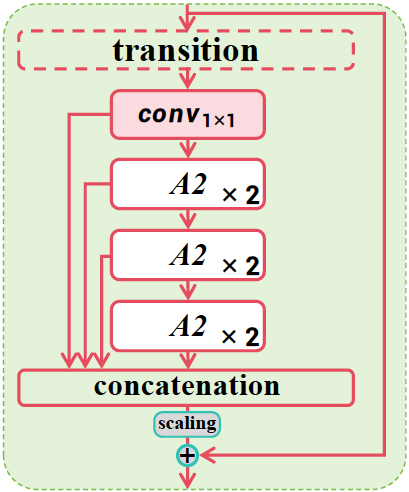
\includegraphics[width=\textwidth]{02-main/figures/ch2/ch2_yolo_09_architecture_relan.png}
        \caption{``R-ELAN'' (YOLOv12)}
        \label{fig:ch2_yolo_09_architecture_relan}
    \end{subfigure}
    \caption{Évolution architecturale des blocs utilisés dans YOLO \cite{tian_yolov12_2025}}
    \label{fig:ch2_yolo_architecture_simplifiee}
\end{figure}

\paragraph{Améliorations architecturales}
\citeauthor{tian_yolov12_2025} introduisent plusieurs optimisations architecturales cruciales pour adapter efficacement les mécanismes d'attention au contexte temps réel de YOLO.

FlashAttention \cite{dao_flashattention_2022} résout le problème fondamental d'accès mémoire des transformers. Traditionnellement, l'attention stocke des matrices intermédiaires volumineuses en mémoire GPU lente (HBM), créant un goulot d'étranglement. FlashAttention optimise ces accès mémoire, réduisant significativement la latence sans perte de précision.

La suppression de l'encodage positionnel simplifie drastiquement l'architecture par rapport aux Vision Transformers classiques. Cette décision contre-intuitive s'avère bénéfique, l'information spatiale est préservée grâce à un ``position perceiver'' (convolution séparable 7×7) appliqué aux valeurs d'attention, plus efficace que les encodages positionnels traditionnels.

La réduction du ratio MLP (Multilayer Perceptron) de 4.0 vers 1.2 rééquilibre la charge computationnelle entre les blocs d'attention et les réseaux feed-forward. Dans les Vision Transformers standards, le MLP consomme 75 \% des calculs ; YOLOv12 privilégie l'attention (plus bénéfique pour la détection) en réduisant la taille des MLP.


\subsubsection{Résultats principaux}
YOLOv12 établit un nouveau compromis vitesse-précision optimal qui démontre la viabilité des mécanismes d'attention pour la détection temps réel.

Les performances surpassent systématiquement les modèles existants. YOLOv12-N atteint 40.6\% mAP en 1.64 ms, dépassant YOLOv11-N de 1.2\% mAP à vitesse équivalente. Cette supériorité se maintient sur toutes les échelles de modèles.

L'efficacité computationnelle est remarquable face aux détecteurs bout-à-bout. YOLOv12-S (9.3 M paramètres) surpasse RT-DETR-R18 \cite{zhao_detrs_2024} (20 M paramètres) avec 42~\% de vitesse supplémentaire. Il utilise seulement 36~\% des calculs et 47~\% des paramètres.

Les cartes d'activation (Figure \ref{fig:ch2_yolo_10_perception}) révèlent une amélioration qualitative notable, avec des contours d'objets plus nets et une activation de premier plan plus précise comparé à YOLOv10/v11, illustrant concrètement les bénéfices des mécanismes d'attention optimisés.

\begin{figure}[H]
    \centering
    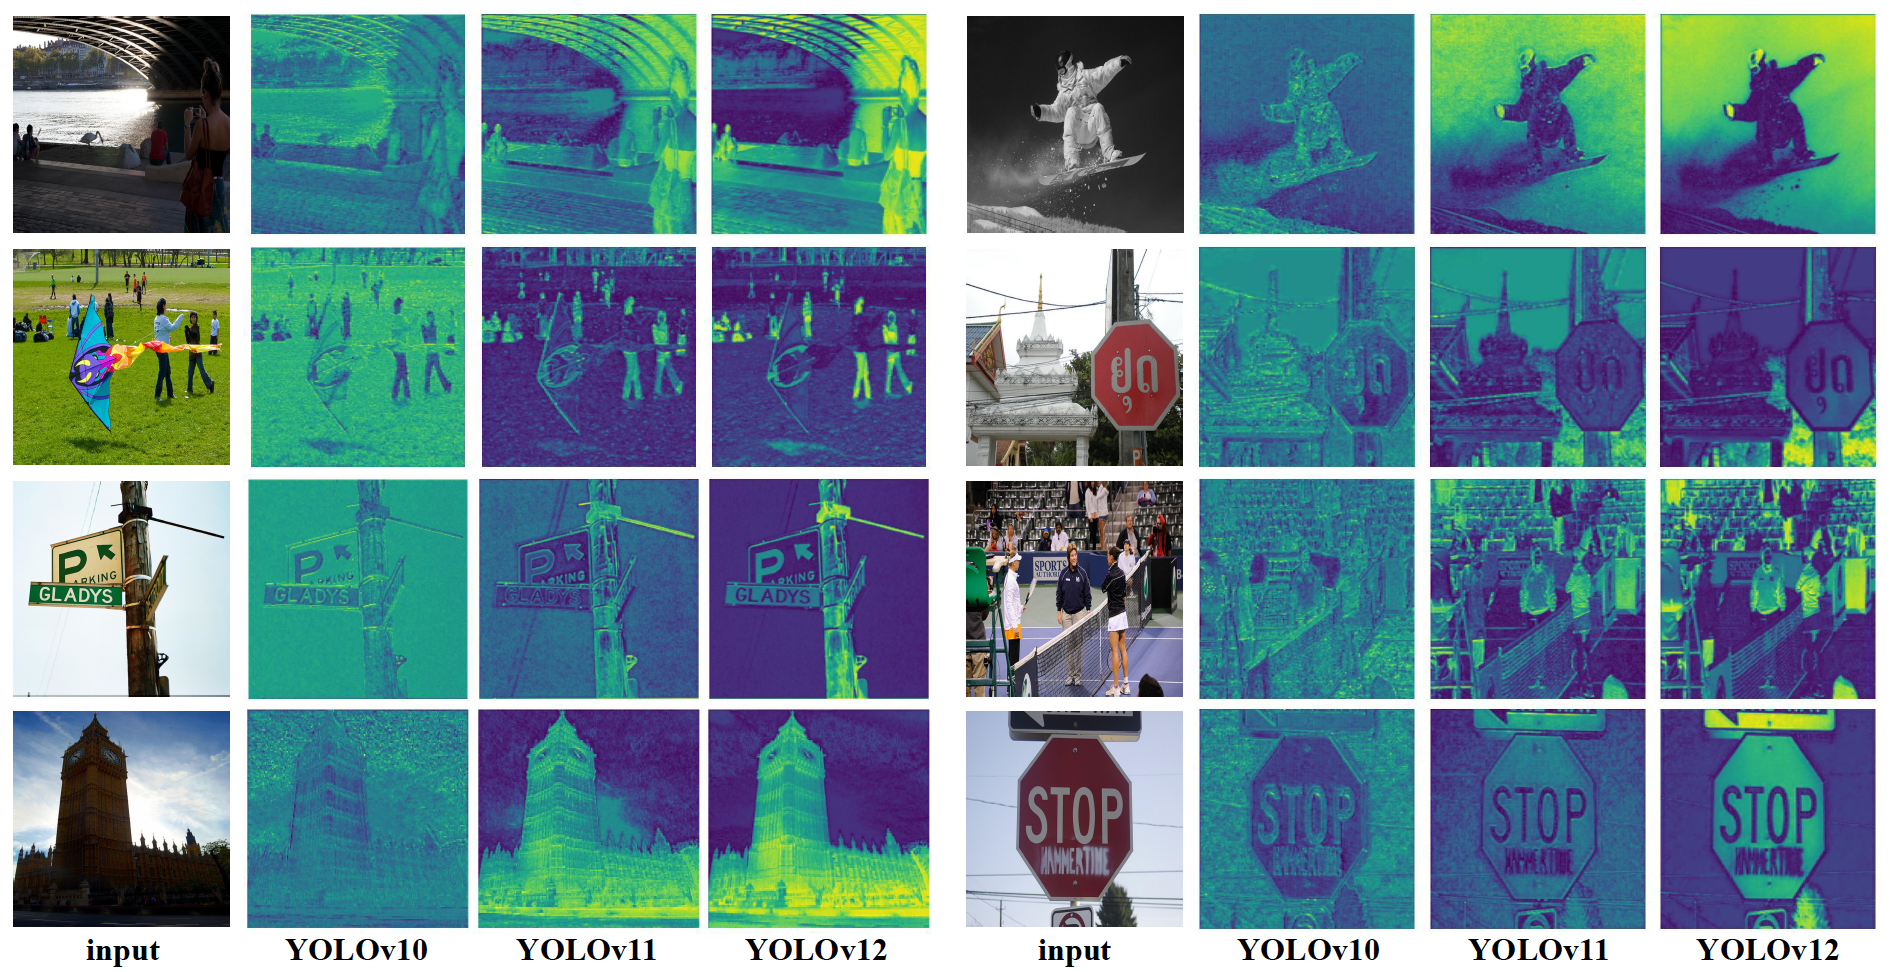
\includegraphics[width=1\linewidth]{02-main/figures/ch2/ch2_yolo_10_perception.png}
    \caption{Perception des objets dans YOLOv10, YOLOv11 et YOLOv12 \cite{tian_yolov12_2025}}
    \label{fig:ch2_yolo_10_perception}
\end{figure}

\subsubsection{Discussion et limites}
YOLOv12 représente une avancée majeure en démontrant que les mécanismes d'attention peuvent être rendus suffisamment efficaces pour la détection temps réel.

Si l'étude démontre théoriquement qu'il est possible de rendre l'attention suffisamment efficace pour la détection temps réel, l'impact pratique reste mitigé. \citeauthor{khanam_review_2025} \cite{khanam_review_2025} révèlent que YOLOv12 est à peine plus performant que ses prédécesseurs avec une architecture relativement complexe et plus gourmande en énergie.

La contrainte matérielle constitue une limitation majeure souvent sous-estimée. La dépendance exclusive à FlashAttention restreint l'utilisation aux GPU d'architecture Turing ou plus récente (RTX 20/30/40, A100, H100), excluant de facto une large base d'utilisateurs équipés de matériel plus ancien. Cette limitation est particulièrement problématique pour les applications industrielles où les cycles de renouvellement matériel sont longs. Cela affecte également les applications edge, dans lesquelles les ressources sont limitées et l'efficience énergétique du modèle est un paramètre critique.

\subsection{Segment}

\subsubsection{Contexte et objectifs}

\subsubsection{Données}

\subsubsection{Méthodologie}

\subsubsection{Résultats principaux}

\subsubsection{Discussion et limites}

\todo[inline]{Ajouter l'état de l'art pour les CNN choisies}
% -----------------------------------------------------------------------------
\subsection{?}

\subsubsection{Contexte et objectifs}

\subsubsection{Données}

\subsubsection{Méthodologie}

\subsubsection{Résultats principaux}

\subsubsection{Discussion et limites}
\todo[inline]{Effacer ça une fois l'état de l'art terminé}

% -----------------------------------------------------------------------------
% -----------------------------------------------------------------------------
\section{Datasets disponibles}
\label{sec:dataset_disponible}
\par{Quelques datasets de qualité sont disponibles actuellement. Ce chapitre va parcourir certains d'entre eux.}

% -----------------------------------------------------------------------------
\subsection{Roof Information Dataset for Computer Vision-Based Photovoltaic Potential Assessment (RID)}
\label{subsec:rid_roof_information_dataset}

\subsubsection{Contexte et objectifs}
\par{Malgré l'existence de dataset pour la segmentation des toitures des bâtiments ou la détection de panneaux solaires, aucun d'entre eux ne permet la segmentation sémantique complète des toitures et de leurs éléments. Dans ce contexte, \citeauthor{krapf_ridroof_2022} présentent le Roof Information Dataset (RID) \cite{krapf_ridroof_2022}, premier dataset public de segmentation de toitures et de leurs éléments.}

\subsubsection{Données}
\par{Le RID se compose d'images aériennes géo-référencées et d'annotations.}
\par{Les images sont des photos aériennes à haute résolution (environ 10 cm/pixel) centrées sur chaque bâtiment, téléchargées via l'API Google Maps Static pour la zone rurale de Wartenberg en Allemagne. Ces images sont géo-référencées au format GeoTIFF.}
\par{Les annotations sont des images rasterisées au format PNG}

\par{Les principaux chiffres-clés de ce dataset :}
\begin{itemize}
    \item 1880 bâtiments uniques répartis sur une zone de 1,5 km² (4,9 km² avec superposition)
    \item 4520 polygones de segments de toiture classés selon leur orientation géographique, en tout 5 classes :
    \begin{itemize}
        \item Nord, sud, est et ouest
        \item Toiture plate
    \end{itemize}
    \item 12359 polygones de superstructures répartis en 9 classes :
    \begin{itemize}
        \item Panneau PV
        \item Lucarne
        \item Fenêtre
        \item Échelle
        \item Cheminée
        \item Ombrage
        \item Arbre/végétation
        \item Fond d'image (background)
        \item Inconnu
    \end{itemize}
\end{itemize}
\par{Les annotations sont fournies en deux versions différentes. La version initiale a été réalisées par cinq annotateurs. Ensuite deux annotateurs supplémentaires ont corrigés et compléter les annotations initiales. La Figure \ref{fig:rid_dataset_image_sample} représente avec une image d'exemple les différences entre les annotations.}

\begin{figure}[H]
    \makebox[\textwidth][c]{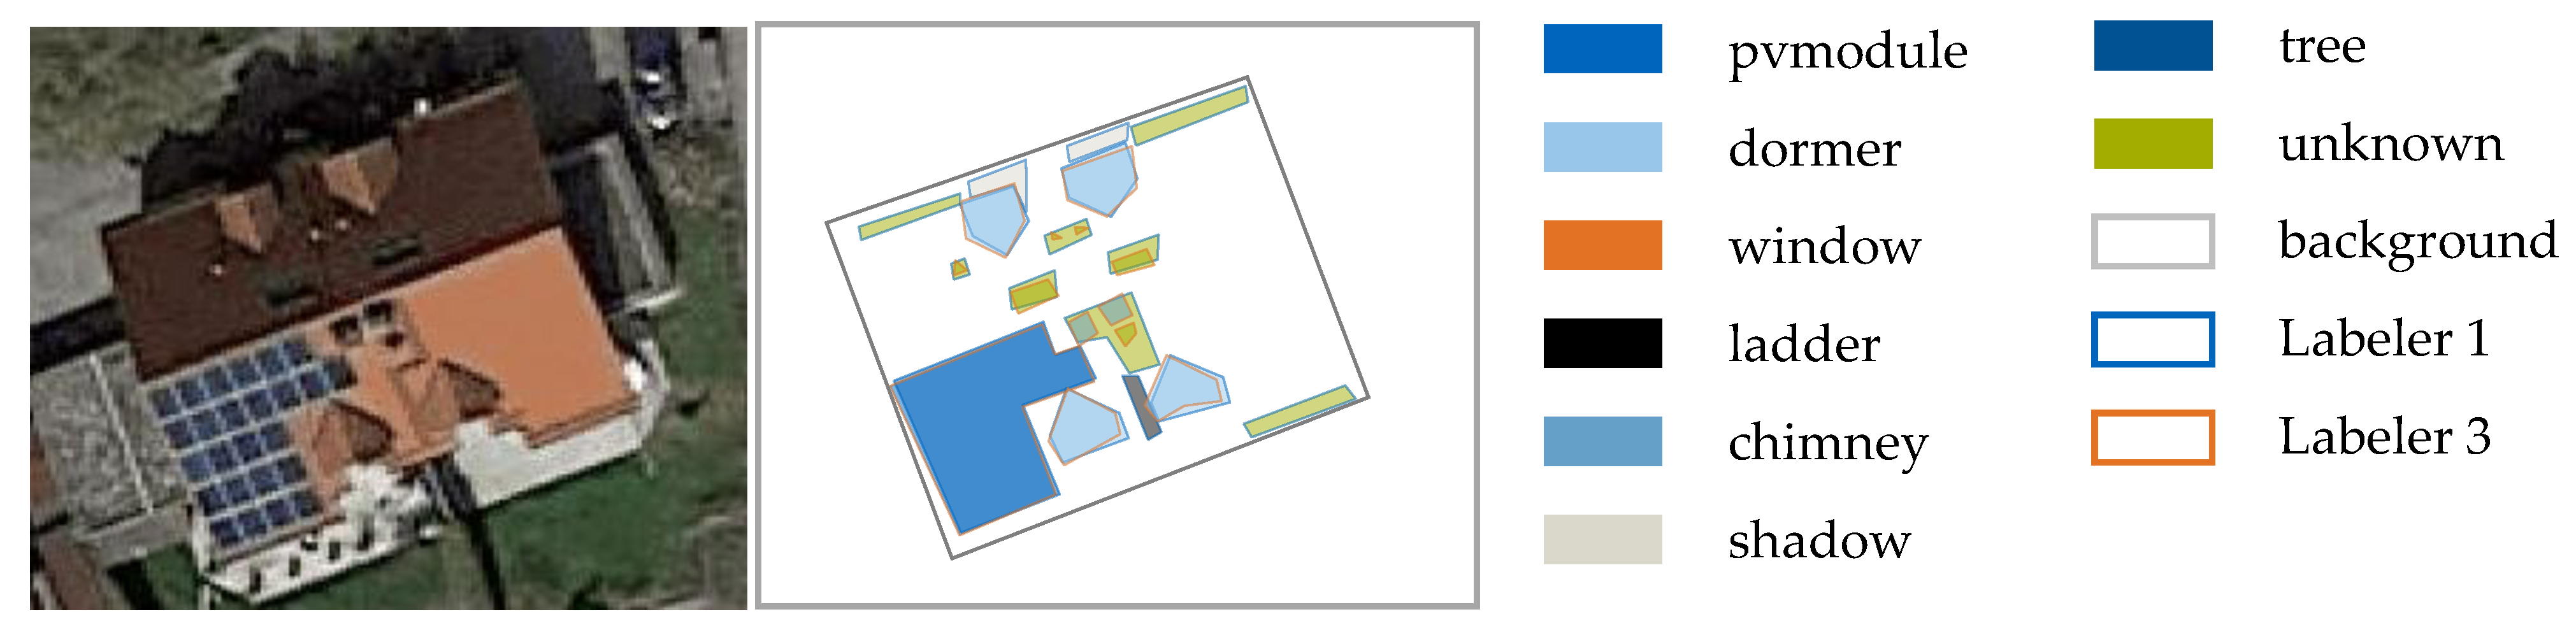
\includegraphics[width=1.15\textwidth]{02-main//figures/ch2/rid_dataset_image_sample.png}}
    \caption{Exemple d'image du dataset, ainsi que les différentes annotations des annotateurs \cite{krapf_rid_2021}}
    \label{fig:rid_dataset_image_sample}
\end{figure}

\par{La Figure \ref{fig:rid_dataset_distribution_classes} représente la distribution des éléments de toiture par classe.}
\begin{figure}[H]
    \centering
    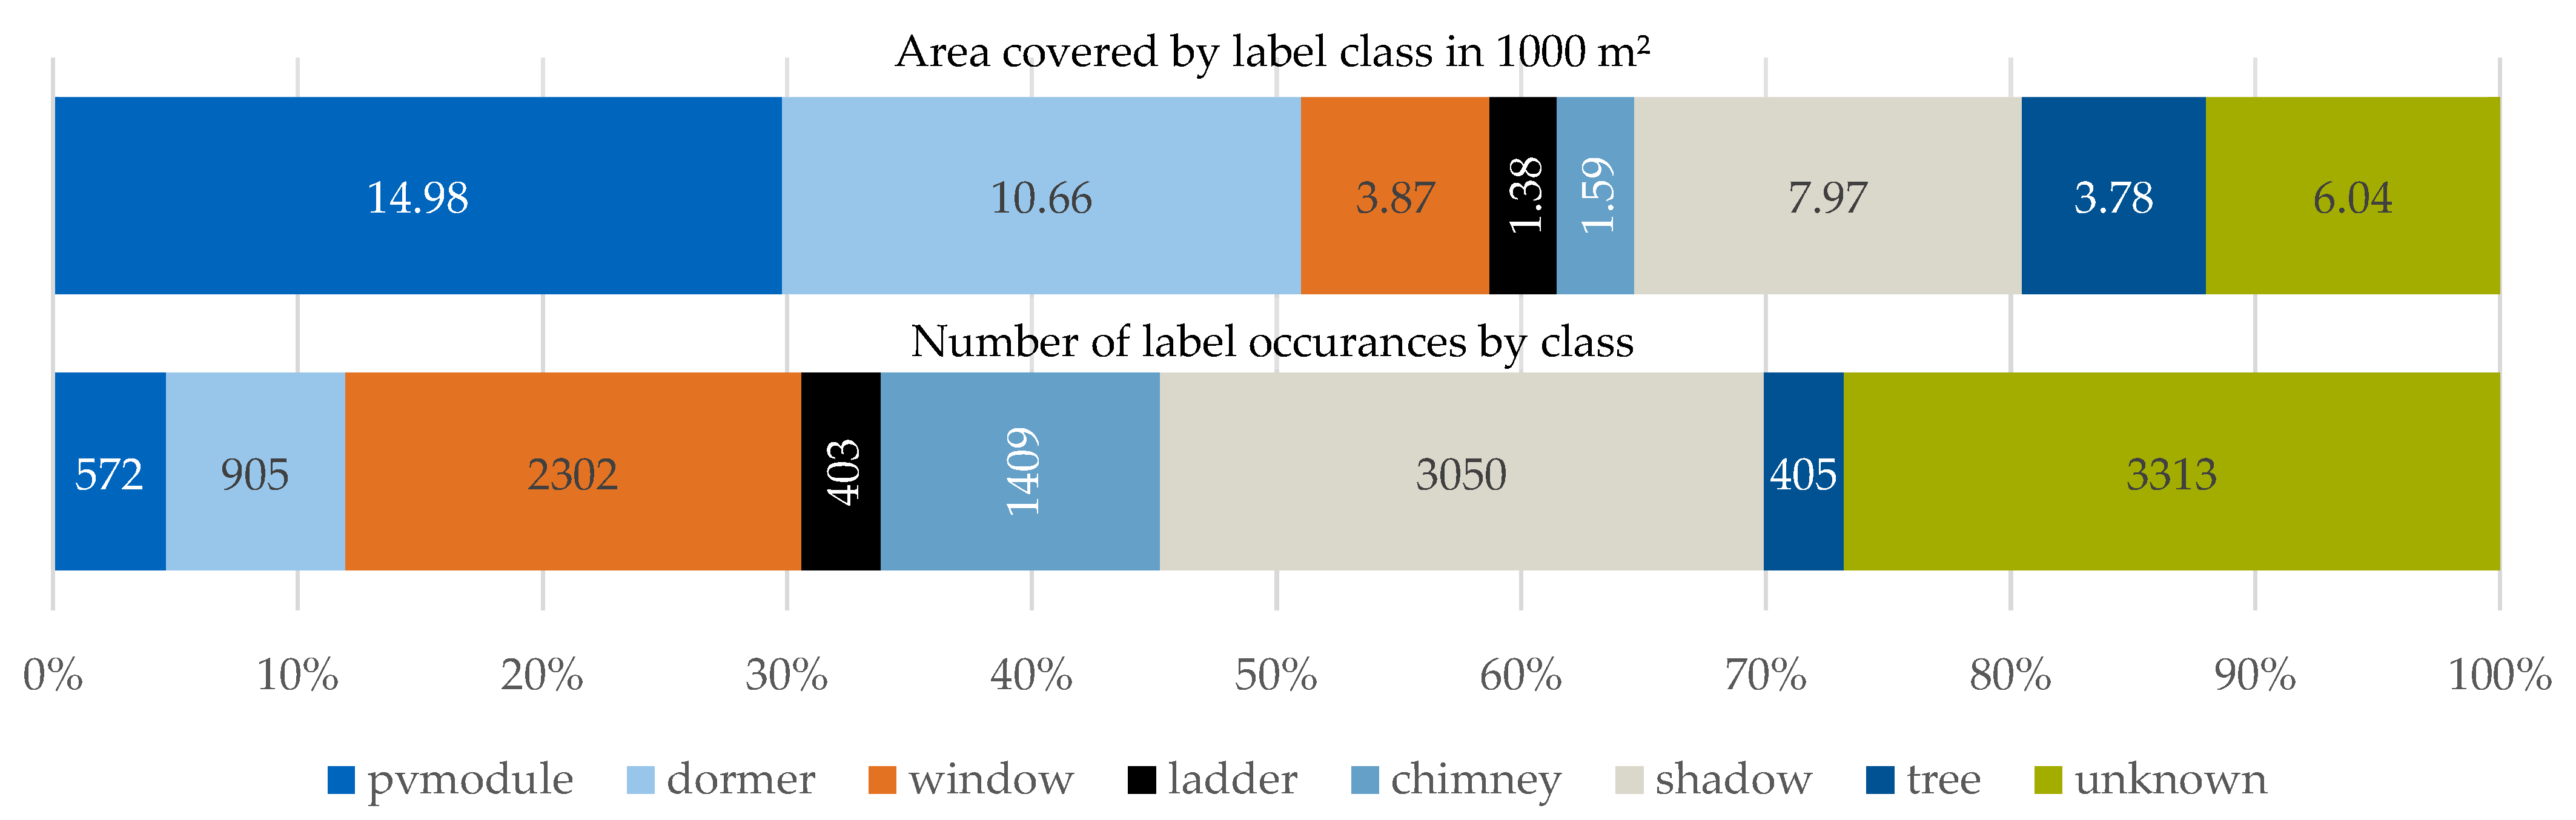
\includegraphics[width=1\linewidth]{02-main//figures/ch2/rid_dataset_distribution_classes.png}
    \caption{Distribution des classes dans le dataset des éléments de toiture \cite{krapf_ridroof_2022}}
    \label{fig:rid_dataset_distribution_classes}
\end{figure}
\par{Le dataset est disponible en ligne \cite{krapf_rid_2021} ainsi que le code \cite{krapf_tumftmrid_2025}.}

\subsubsection{Méthodologie}
\par{Le processus de création du dataset s'est déroulé en plusieurs phases :}
\begin{enumerate}
    \item Sélection de la zone d'étude :
    \begin{itemize}
        \item Zone rurale de Wartenberg (Munich) choisie pour offrir des images de qualité variable (contraste, ombres, distorsions) afin d'améliorer la capacité des modèles à s'adapter à des conditions variables
    \end{itemize}
    \item Acquisition des données :
    \begin{itemize}
        \item Téléchargement d'images aériennes via l'API Google Maps
        \item Résolution d'environ 10 cm/pixel, suffisante pour identifier les petites éléments présents sur les toitures comme les cheminées
    \end{itemize}
    \item Processus d'annotation initial :
    \begin{itemize}
        \item Développement d'un outil d'annotation personnalisé permettant de dessiner des polygones sur l'interface Google Maps Dynamic API
        \item Annotation par cinq membres universitaires suivant un ensemble de règles prédéfini
        \item Deux tâches d'annotation distinctes : segments de toiture (classes N, S, W, O, plat) et les éléments présents sur les toitures.
    \end{itemize}
    \item Évaluation de la qualité d'annotation :
    \begin{itemize}
        \item Expérience d'annotation comparative sur 26 bâtiments sélectionnés pour contenir au moins 15 occurrences de chaque classe de superstructure
        \item Analyse de l'accord entre annotateurs pour identifier les classes les plus difficiles à annoter
    \end{itemize}
    \item Processus de révision :
    \begin{itemize}
        \item Utilisation de l'outil CVAT (Computer Vision Annotation Tool) permettant un zoom plus important
        \item Révision par deux annotateurs n'ayant pas participé à l'annotation initiale pour limiter les biais
        \item Attention particulière aux classes ayant montré un faible accord inter-annotateurs
    \end{itemize}
    \item Répartition manuelle des données en dataset d'entraînement, validation et test :
    \begin{itemize}
        \item Division géographique (et non aléatoire) pour éviter le chevauchement entre ensembles d'entraînement et de test
        \item Création de cinq configurations de partitionnement différentes pour la validation croisée (cross-validation)
    \end{itemize}

    \item Application à l'estimation du potentiel photovoltaïque :
    \begin{itemize}
        \item Entraînement de réseaux de neurones (U-Net et Panoptic FPN) pour la détection des éléments de toiture
        \item Conversion des masques de segmentation en géométries vectorielles
        \item Calcul du potentiel photovoltaïque en tenant compte des éléments de toiture
    \end{itemize}
\end{enumerate}

\subsubsection{Résultats principaux}
L'article présente plusieurs catégories de résultats :
\begin{enumerate}
    \item Qualité des annotations :
    \begin{itemize}
        \item Forte variabilité de l'accord inter-annotateurs (IoU) selon les classes
        \item Classes avec bon accord : lucarnes (0,70) et panneaux solaires (0,68)
        \item Classes problématiques : objets inconnus (0,15), échelles (0,22)
        \item IoU moyen global de 0,48 pour l'annotation initiale et performance plus élevée après révision
    \end{itemize}
    \item Performances des réseaux de neurones :
    \begin{itemize}
        \item U-Net et Panoptic FPN entraînés et testés sur les deux versions du dataset
        \item Meilleure performance : U-Net avec IoU moyen de 0,42-0,44 sur le jeu de test initial
        \item Performance améliorée à 0,45-0,46 sur les annotations révisées
        \item Réseaux capables de compenser partiellement les incohérences d'annotation
        \item Détection performante des panneaux solaires (IoU 0,69) et lucarnes (IoU 0,60)
    \end{itemize}
    \item Impact sur l'évaluation du potentiel photovoltaïque :
    \begin{itemize}
        \item La prise en compte des éléments de toiture réduit significativement le potentiel PV estimé
        \item Réduction de 20,5\% avec annotations manuelles et 15,0\% avec prédictions du réseau
        \item Avec une approche de placement réaliste des modules, réduction de 31,1\%
        \item Impact très variable selon les toitures : de moins de 5\% pour 39\% des toits à plus de 70\% pour 10\% des toits
        \item L'exclusion des segments déjà équipés de panneaux solaires réduit le potentiel de 29,5\%
    \end{itemize}
\end{enumerate}
\par{Ces résultats démontrent l'importance de considérer les éléments de toiture dans l'évaluation du potentiel solaire des toitures et valident l'approche par apprentissage profond sur images aériennes comme alternative viable aux méthodes basées sur \gls{lidar}, malgré les défis liés à la qualité des annotations.}

\subsubsection{Discussion et limites}
\par{Le dataset se concentre sur une zone rurale allemande et ne représente pas adéquatement d'autres styles architecturaux. Comme indiqué dans la section \ref{subsec:solar_net_plus} qui fait référence a un article postérieur du même auteur, le dataset n'est pas adapté au milieu urbain de Bruxelles. Les classes sont trop spécifiques au rural allemand, dans le cas de Bruxelles, il manque les classes pour des éléments typiquement urbains tel que les ventilation/climatisation.}
\par{Il y a une forte disproportion entre les classes d'éléments de toiture, avec certaines classes très peu représentées et d'autres classes étant dans toutes les images (cas classe "background").}
\par{L'article s'intéresse aussi à la variabilité de la qualité d'annotation. Les annotateurs ne sont pas toujours d'accord sur les annotations (polygone) et les classes. La qualité des annotations a un impact sur la performance des modèles. Les variations dans les annotations sont aussi en partie dues a la résolution des images, celle-ci peux être insuffisante pour clairement identifier et annoter les petits objets.}
\par{Les résultats des deux modèles sont encourageants, mais doivent être pris comme point de départ pour améliorer la qualité du dataset.}

% -----------------------------------------------------------------------------
\subsection{Autres dataset}

\par{Le dataset de la section précédente est le seul disponible en ligne qui permet de faire de la segmentation sémantique des éléments de toiture. La plupart des articles ne partagent pas leur dataset, plusieurs hypothèses sont possible:}
\begin{itemize}
    \item Contraintes contractuelles avec les fournisseurs d'images qui limitent leur diffusion
    \item Les datasets annotés représentent un investissement considérable en temps et ressources, constituant un capital intellectuel précieux pour de futures publications ou demandes de financement.    
    \item Difficultés liées au stockage et à la distribution de volumes importants de données géospatiales, ainsi qu'à la maintenance d'une infrastructure adéquate pour supporter l'accès externe.
    \item L'effort nécessaire pour documenter, nettoyer et préparer un dataset à usage public dépasse souvent les ressources disponibles ou allouées dans le cadre du projet initial.
    \item Manque de reconnaissance académique formelle pour le partage de données comparativement aux publications d'articles, et parfois politiques institutionnelles restrictives concernant la propriété intellectuelle.
\end{itemize}
\par{La section suivante décrit les datasets disponibles pour les panneaux solaire PV, cela reste tout de même en lien avec l'identification des éléments de toiture.}

\subsubsection{Datasets dédiés aux panneaux solaires PV}
\par{Plusieurs datasets spécifiques à la détection et segmentation des panneaux solaires photovoltaïques sont disponibles dans la littérature scientifique. La plateforme Roboflow Universe \cite{roboflow_roboflow_nodate}, qui héberge plus de 500'000 datasets, propose une dizaine de datasets dédiés à la segmentation sémantique ou à la classification des panneaux solaires. Cependant, ces datasets présentent généralement des limitations importantes: nombre restreint d'images et annotations de qualité variable.}
\par{Parmi les datasets plus significatifs, celui publié par \citeauthor{kasmi_crowdsourced_2023} \cite{kasmi_crowdsourced_2023, kasmi_crowdsourced_2022} se distingue par son approche collaborative. Son objectif principal est la détection binaire de panneaux solaires PV dans des images satellite. Ce dataset a la particularité d'avoir été prévu pour être enrichi continuellement grâce à un système de labellisation participatif accessible via GitHub \cite{gabrielkasmi_gabrielkasmibdappv_2025}. À ce jour, il recense environ 28'000 installations photovoltaïques sur plus de 33'000 images satellite. Ses sources de données sont l'IGN (Institut national de l'information géographique et forestière) ainsi que Google.}
\par{Un autre dataset notable a été publié par \citeauthor{thebault_comprehensive_2025} \cite{thebault_comprehensive_2025}. Baptisé FRPV \cite{thebault_frpv_2025}, ce dataset a été utilisé pour évaluer le potentiel solaire photovoltaïque en France. Il combine des images provenant de l'IGN et de Google Maps, pour un total de 23'709 images contenant des installations photovoltaïques et 45'418 images sans installation PV, offrant ainsi un corpus équilibré pour l'entraînement de modèles de classification.}

% -----------------------------------------------------------------------------
% -----------------------------------------------------------------------------
\section{Solutions commerciales existantes}
\par{Quelques entreprises offrent des solutions pour réaliser un cadastre solaire sur la base de leur données. Dans tous les cas leur méthodologie ou les données utilisées ne sont pas disponible.}
\par{Solargis \cite{solargis_regional_nodate} est un société spécialisée dans le solaire. Cette entreprise offre diverses solutions pour planifier toutes les phases de chantier, depuis la modélisation d'un site jusqu'au suivi et à l'optimisation des performances des panneaux solaires en phase d'exploitation. Ils offrent aussi la prestation de création d'un cadastre solaire pour une région.}
\par{L'entreprise Picterra \cite{picterra_infrastructure_nodate} offre des solutions pour l'utilisation de machine learning sur des données géomatiques. Entre autres, ils proposent l'estimation du potentiel solaire d'une région. Une autre entreprise suisse, Urbio, \cite{urbio_urbio_nodate} offre aussi des prestations similaires à Picterra mais plus axées sur la planification énergétique.}
\par{Google Projet Sunroof \cite{google_project_nodate} exploite les données de Google pour évaluer le potentiel solaire des différentes régions. Cette plateforme propose également quelques conseils pour l'obtention de subventions. Bien que les données générées soient accessibles au public, Google ne les produit que pour les municipalités et régions qui souscrivent à leurs services. Cette solution est actuellement limitée aux USA.}

% -----------------------------------------------------------------------------
% -----------------------------------------------------------------------------
\section{Synthèse}

\par{L'analyse de l'état de l'art révèle trois approches principales pour l'évaluation du potentiel solaire des toitures, chacune présentant des avantages et limitations spécifiques.}

\par{Les méthodes traditionnelles basées sur les données \gls{lidar} et cadastrales, illustrées par les cadastres solaires genevois et suisse (ToitSolaire), offrent une couverture territoriale complète et disposent des validations nécessaires du point de vue académique. Cependant, elles souffrent des mêmes limitations, il n'y pas actuellement de cartographie précise des toitures. Par conséquent, sans la prise en compte de tous les obstacles présents sur les toitures, le potentiel solaire sera surestimé.}

\par{Les approches par machine learning supervisé, exemplifiées par les travaux de \citeauthor{castello_quantification_2021} et \citeauthor{li_deep_2024}, démontrent une capacité prometteuse à identifier automatiquement les surfaces disponibles et les obstacles sur les toitures. Ces méthodes atteignent des performances satisfaisantes (IoU de 64\% pour \citeauthor{castello_quantification_2021}, \%RMSE de 19,92\% pour SolarNet+) mais restent limitées par la disponibilité et la qualité des données d'entraînement annotées.}

\par{L'étude du \acrshort{stdl} illustre la complémentarité des différentes sources de données (\gls{lidar}, orthophotos, données vectorielles) et techniques (classification, segmentation). La combinaison par concaténation des résultats de segmentation \gls{lidar} et d'images atteint un F1-score de 0.79 avec un recall de 0.94, démontrant l'intérêt d'approches hybrides.}

\par{Concernant les données disponibles, le dataset RID constitue actuellement la seule ressource publique permettant la segmentation sémantique complète des éléments de toiture. Cependant, sa limitation à un contexte rural allemand restreint sa généralisation à d'autres environnements urbains.}

\par{Les limites identifiées pointent vers la nécessité de combiner les approches traditionnelles éprouvées avec les techniques de machine learning, condition nécessaire au développement de datasets couvrant une plus grande diversité architecturale. L'exploitation conjointe d'images aériennes et d'informations géomatiques plus poussée s'impose comme l'approche la plus prometteuse pour obtenir un cadastre solaire fiable.}